% CREATED BY DAVID FRISK, 2016
\chapter{Results}

\epigraph{ \textit{If you can not measure something, you can not improve it.}}{--- \textup{William Thomson Kelvin}}

\section{Evaluation metrics}
Generally speaking in Computer Science, every domain and application could have different evaluation metrics, for example the energy efficient of a CPU is a heavy metrics in embedded systems while in a high performant CPU latency and throughput are dominant metrics. As said that, evaluation metrics strongly depend on the end-users, therefore the designers have to make assumption on the end-user intentions and applications.\\
In this work the assumptions are that the accelerator will be deployed into an embedded system and at the same time it should give to the user a certain degree of flexibility for running Neural Network models. Thus, as it is suggested \cite{paper:1} the following metrics are used:
\begin{itemize}
\item Accuracy, quality of the final result of inference process.
\item Throughput, for measuring real time performance. It depends on the number of internal computation cores.
\item Latency, for interactive applications.
\item Energy and Power.
\item Hardware cost (Utilization Factor in case of an FPGA) of chip area and process technology.
\end{itemize}
\newpage
\section{Utilization Factor}
An important aspect of an embedded system is the on-die utilization area. Those kinds of system are usually deployed on tight area-constrained chips for hiding their presence to the user.
Therefore, it is important to measure and understand the behavior on the Utilization of the FPGA (used as area measurement in this case) of the design as the size of Matrix Multiplication Unit increases and in parallel the throughput.\\
The Utilization Factor, composed of Look-up-Table, Flip Flops and Digital Signal Processor usage, is expected to increase as the size of Multiplication Matrix increase and the bit width of Computation Unit.\\
In the following Figures, utilization results are presented for each data type, where the Matrix Multiplication Unit sizes are pushed as much as the timing requirements are meet:
\begin{itemize}
\item Integer 8 bit:
\begin{figure}[!htbp]
\centering
\captionsetup{justification=centering}
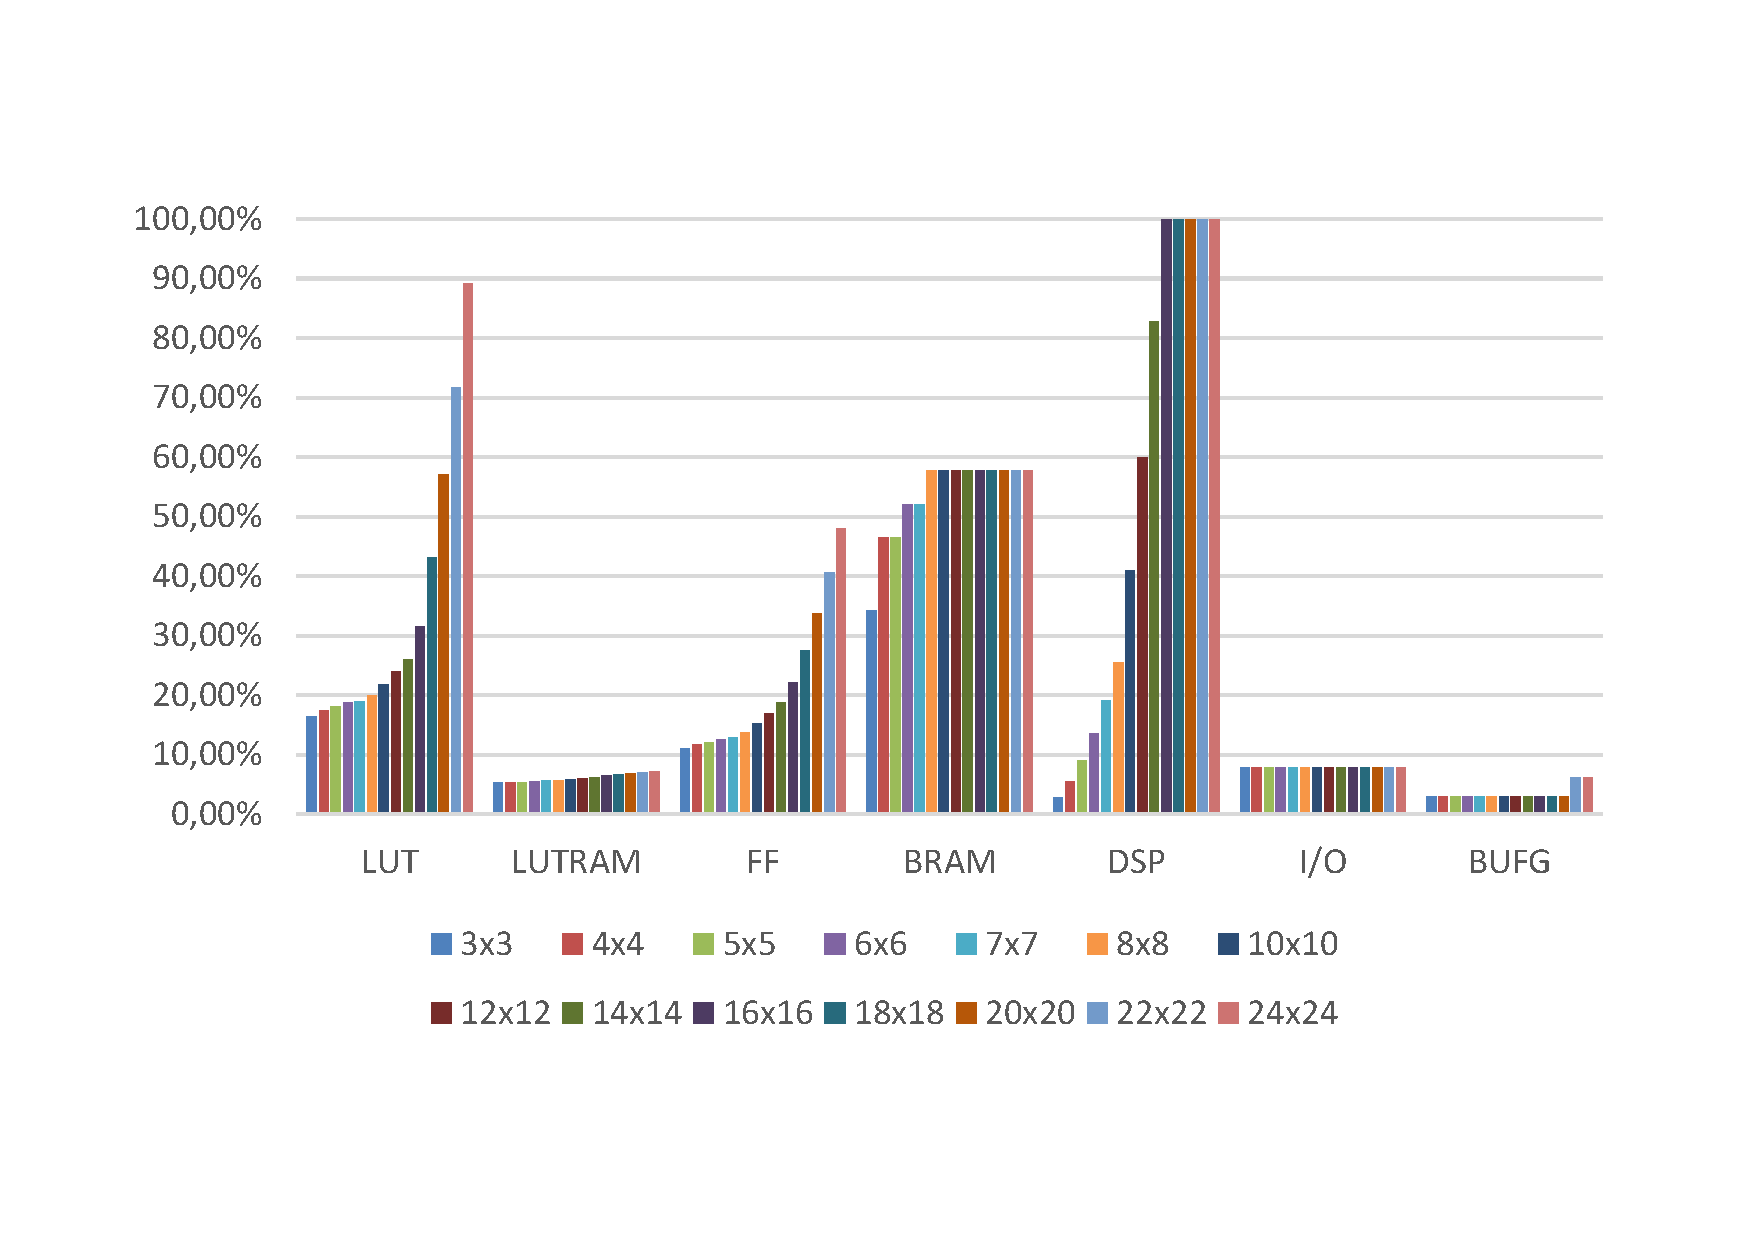
\includegraphics[scale=0.35,angle=0]{./figure/graphs/utilization_factor_30mhz_int8.pdf}
\caption{Post Implementation Utilization Factor of integer 8 bit PEs and clock frequency of 30 Mhz}
\label{fig:ut8bit}
\end{figure}
\item Integer 16 bit:
\begin{figure}[!htbp]
\centering
\captionsetup{justification=centering}
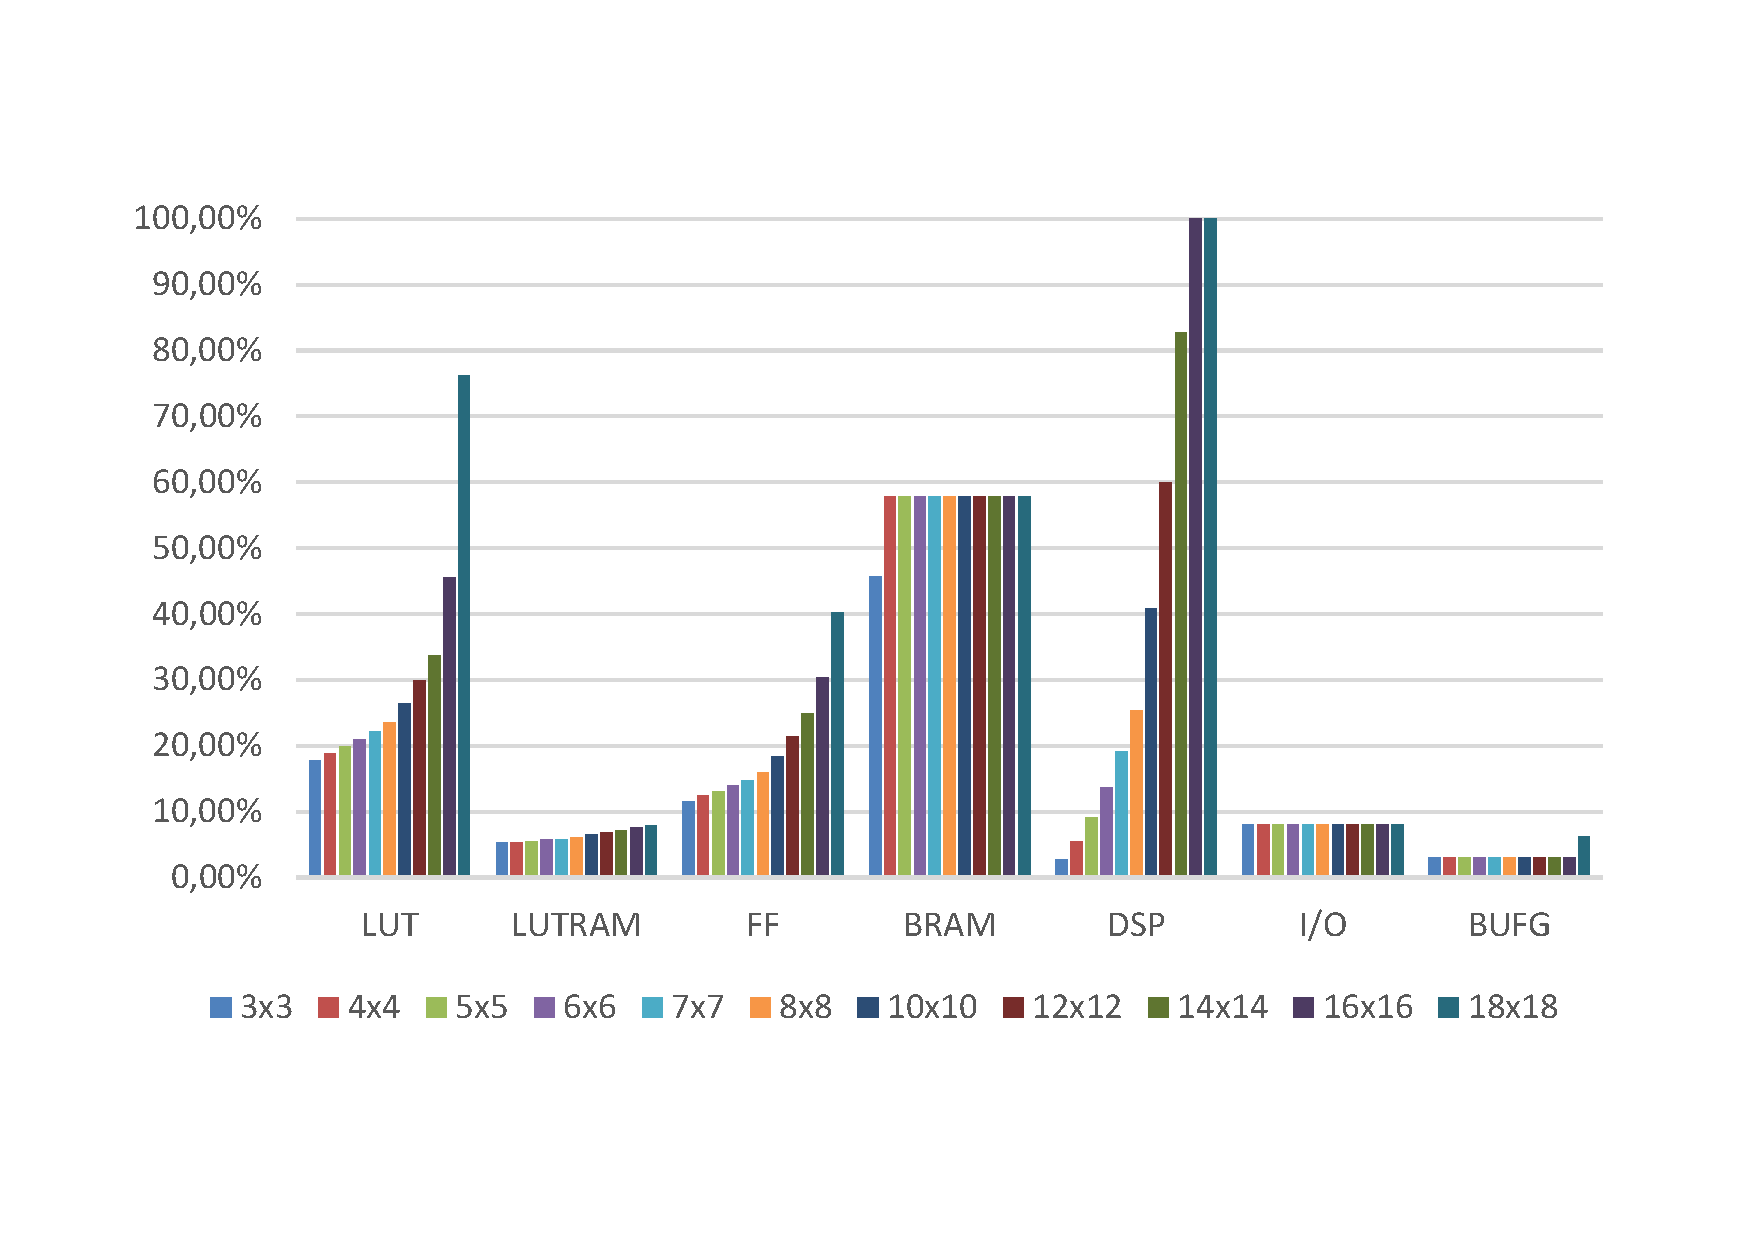
\includegraphics[scale=0.35,angle=0]{./figure/graphs/utilization_factor_30mhz_int16.pdf}
\caption{Post Implementation Utilization Factor of integer 16 bit PEs and clock frequency of 30 Mhz}
\label{fig:ut16bit}
\end{figure}
\newpage
\item Integer 32 bit:
\begin{figure}[!htbp]
\centering
\captionsetup{justification=centering}
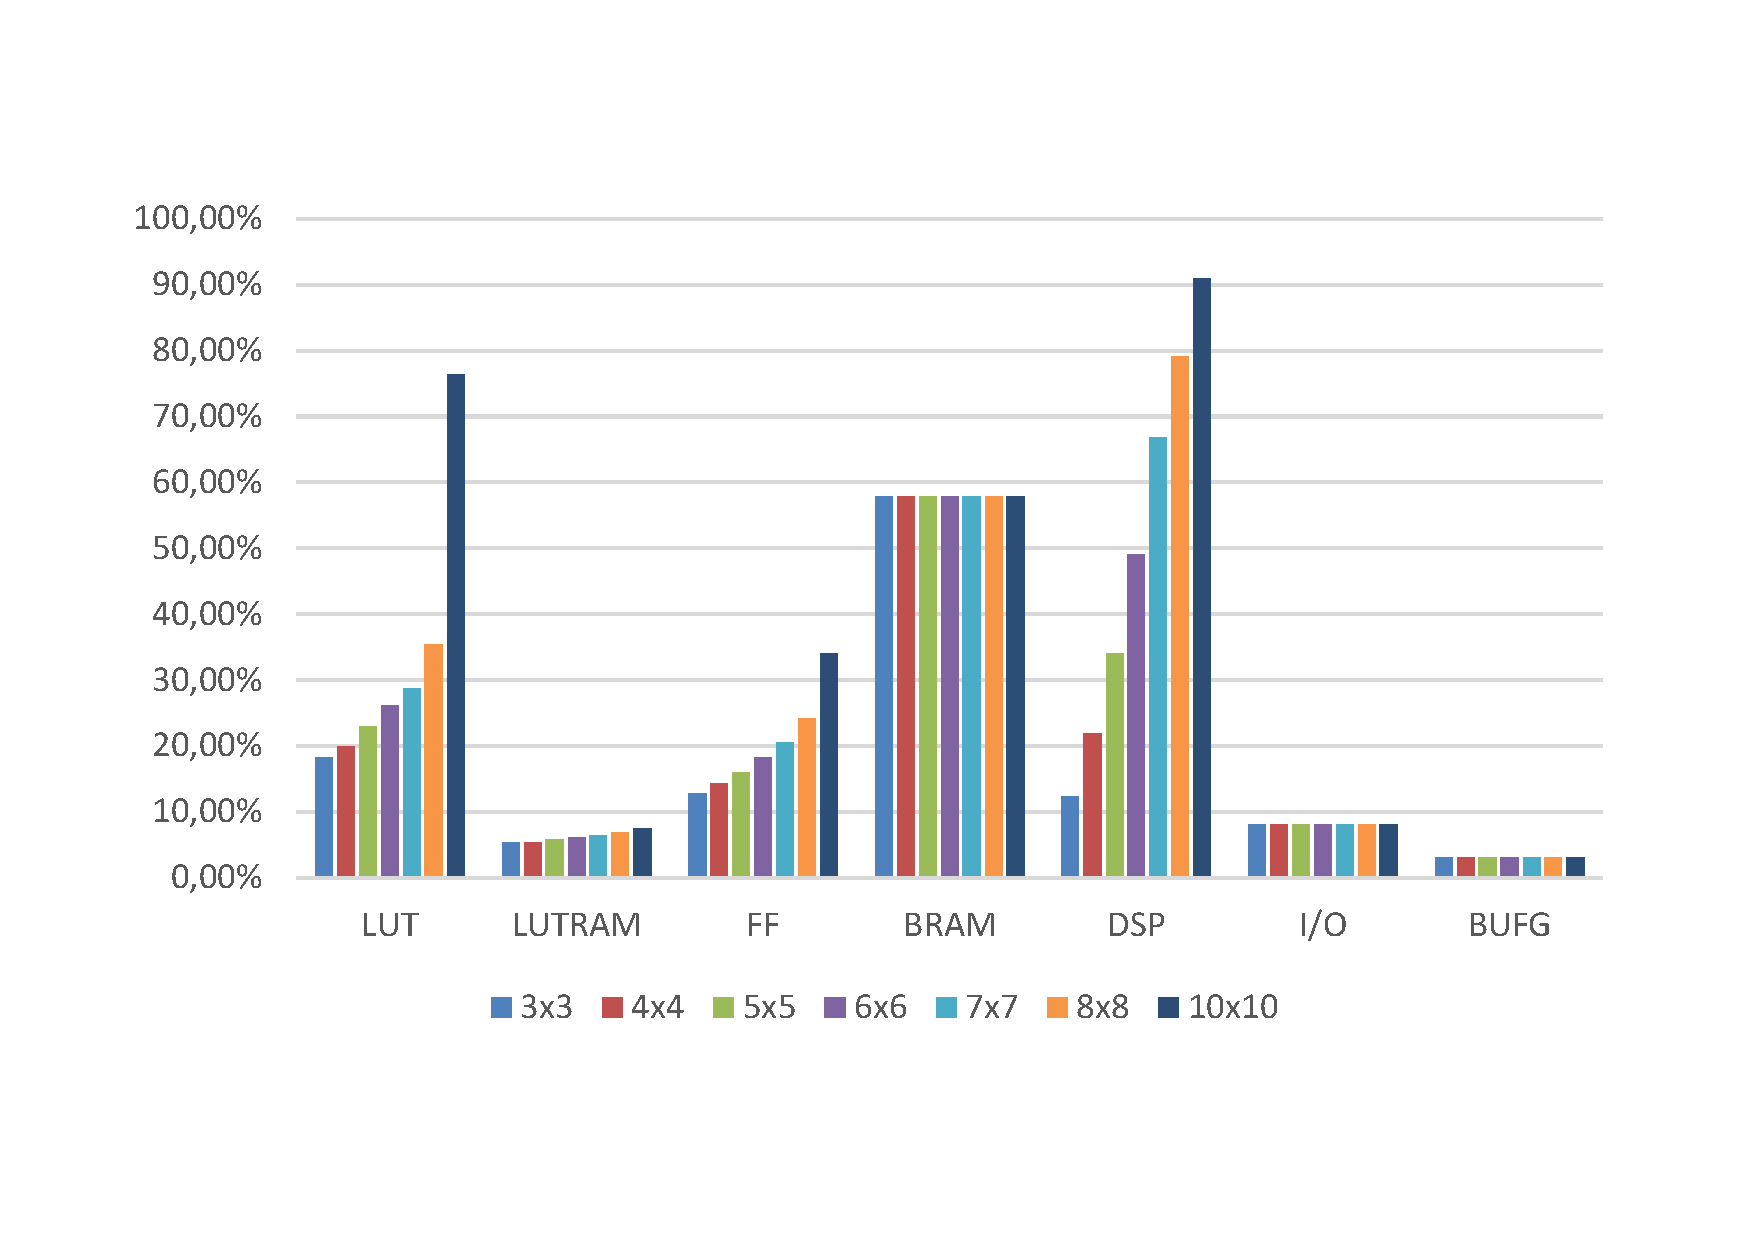
\includegraphics[scale=0.35,angle=0]{./figure/graphs/utilization_factor_30mhz_int32.pdf}
\caption{Post Implementation Utilization Factor of integer 32 bit PEs and clock frequency of 30 Mhz}
\label{fig:ut32bit}
\end{figure}
\item Integer 64 bit:
\begin{figure}[!htbp]
\centering
\captionsetup{justification=centering}
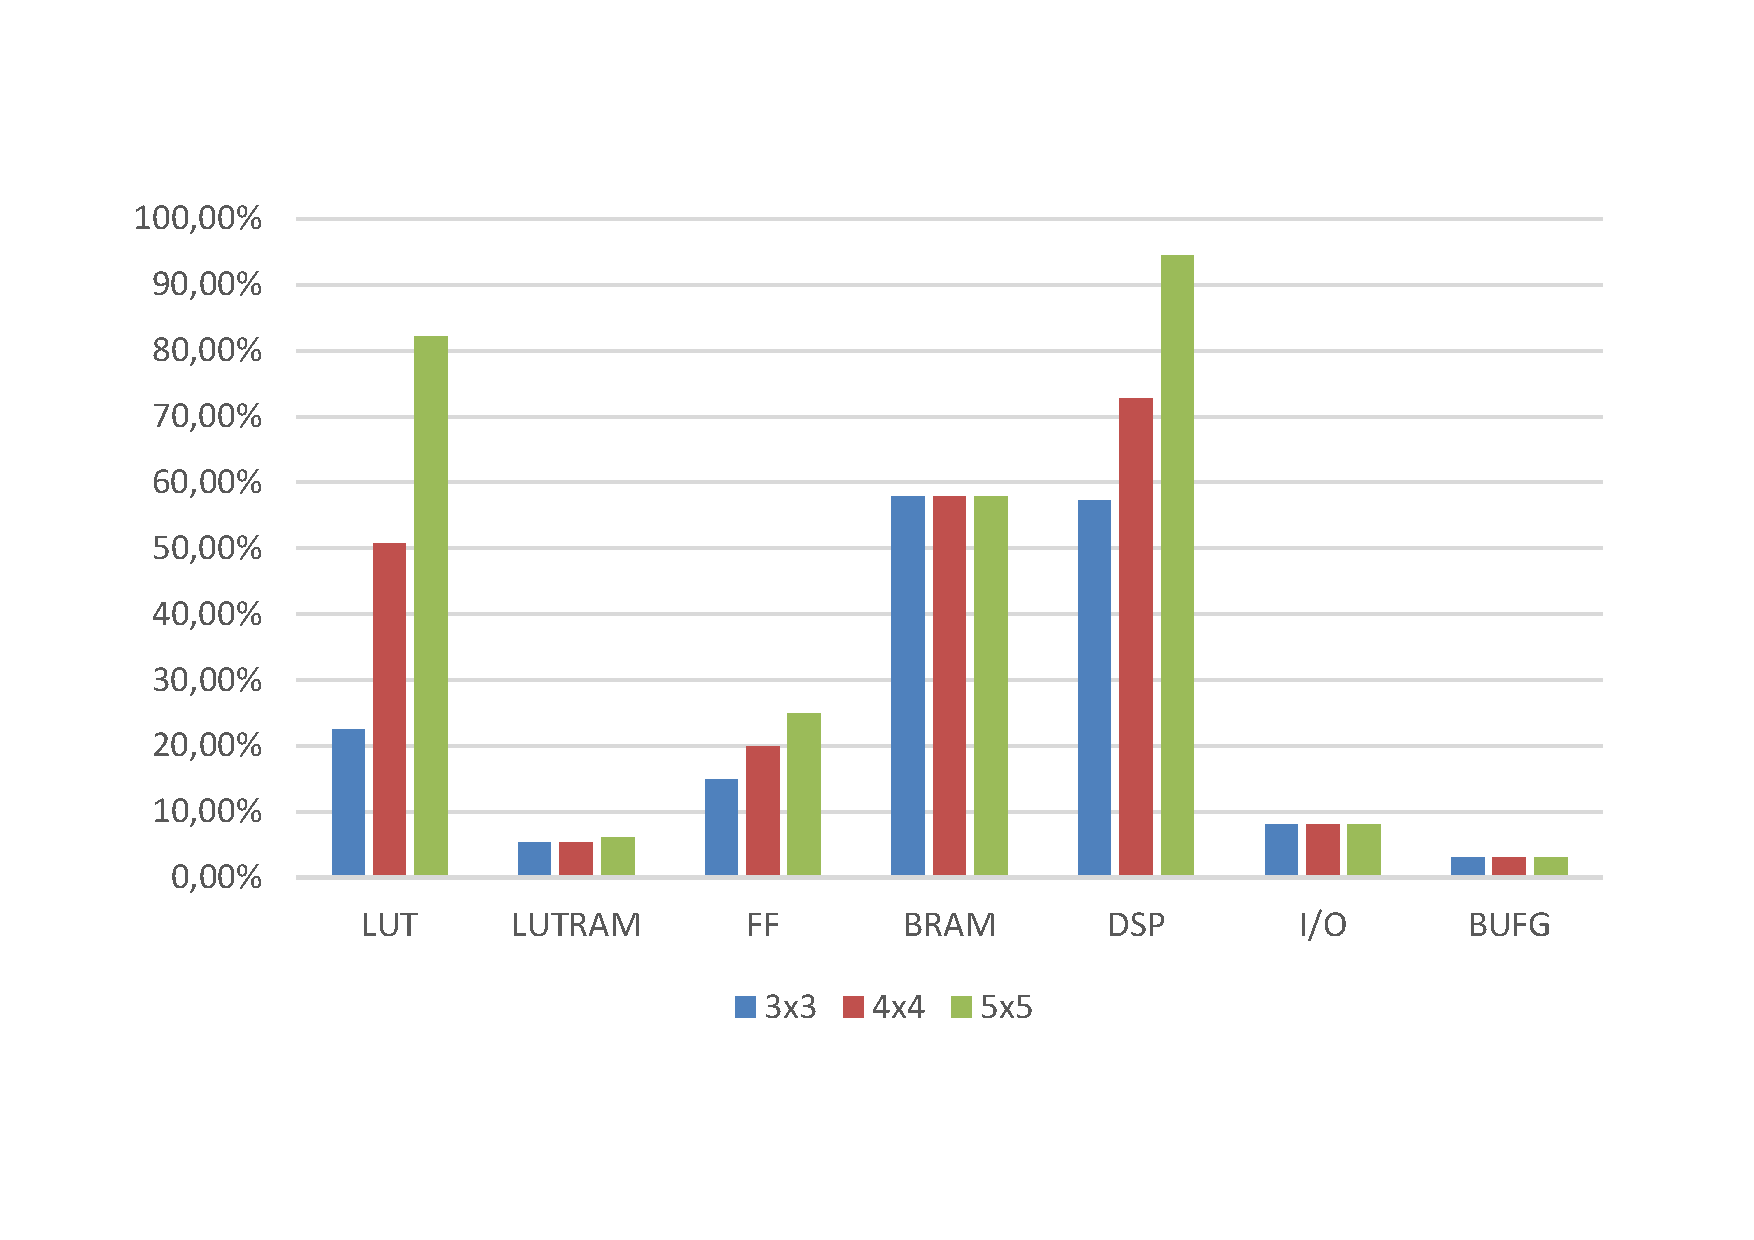
\includegraphics[scale=0.35,angle=0]{./figure/graphs/utilization_factor_30mhz_int64.pdf}
\caption{Post Implementation Utilization Factor of integer 64 bit PEs and clock frequency of 30 Mhz}
\label{fig:ut64bit}
\end{figure}
\item Brain Floating point 16:
\begin{figure}[!htbp]
\centering
\captionsetup{justification=centering}
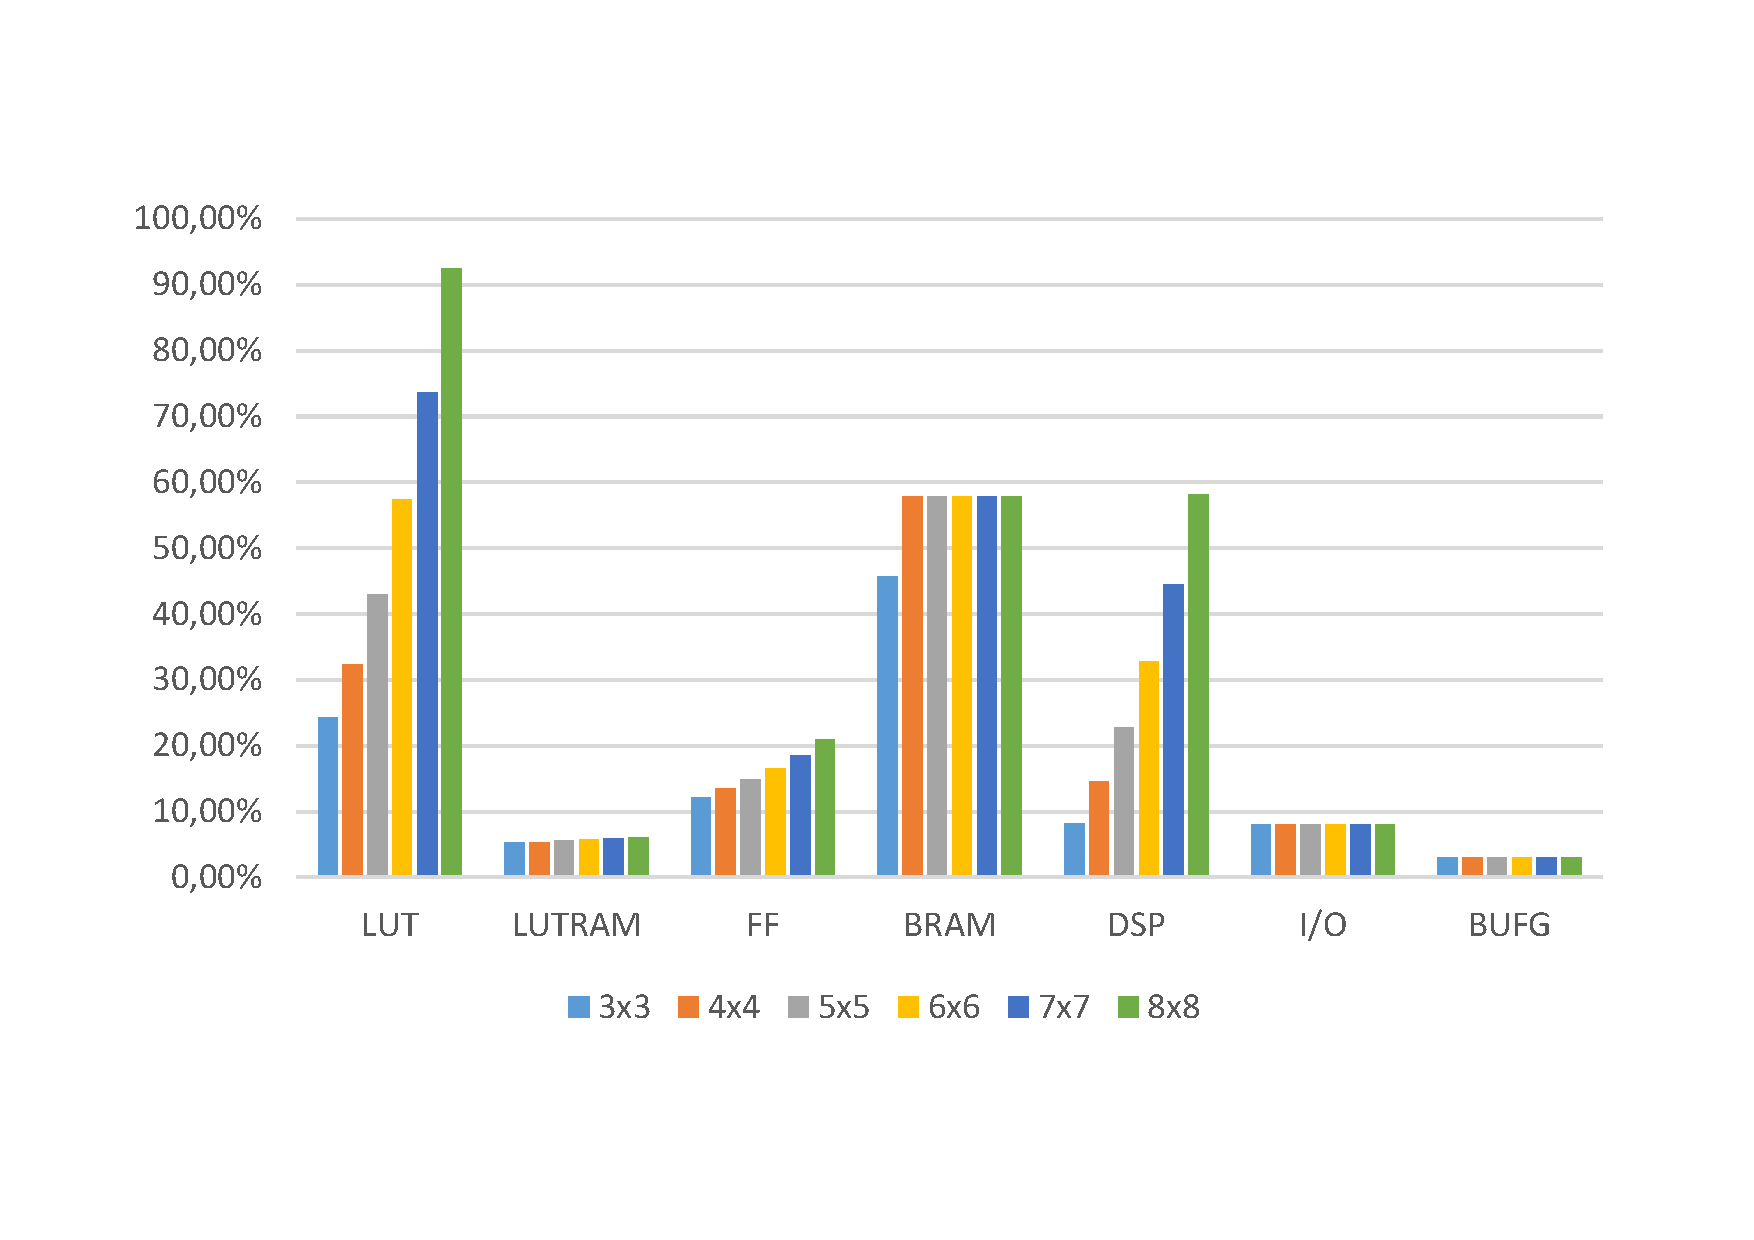
\includegraphics[scale=0.35,angle=0]{./figure/graphs/utilization_factor_30mhz_bfp16.pdf}
\caption{Post Implementation Utilization Factor of bfp 16 bit PEs and clock frequency of 30 Mhz}
\label{fig:utbpf16bit}
\end{figure}
\newpage
\item Floating point 32:
\begin{figure}[!htbp]
\centering
\captionsetup{justification=centering}
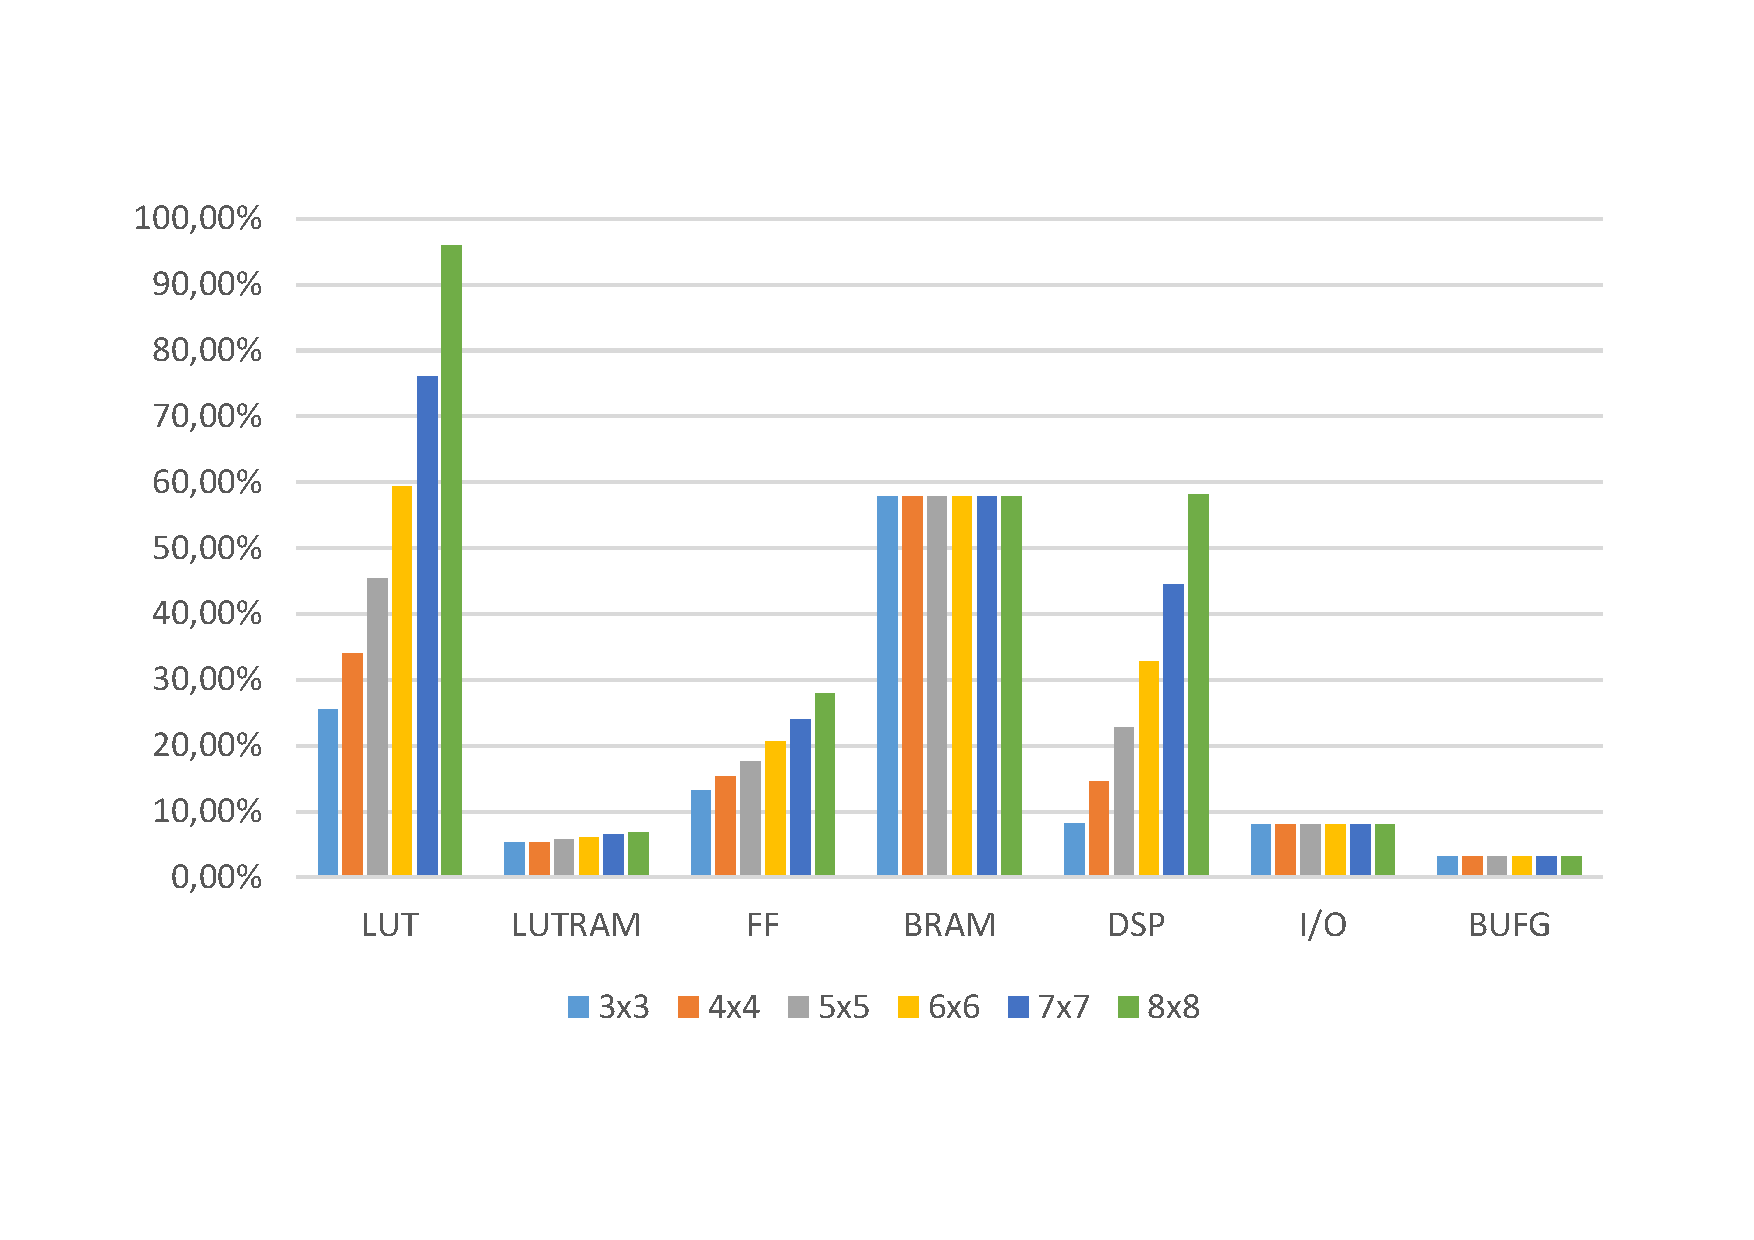
\includegraphics[scale=0.35,angle=0]{./figure/graphs/utilization_factor_30mhz_fp32.pdf}
\caption{Post Implementation Utilization Factor of fp 32 bit PEs and clock frequency of 30 Mhz}
\label{fig:utfp32bit}
\end{figure}
\end{itemize}
It can be seen that the trend for integer 8 and 16 is similar (Figure \ref{fig:ut8bit} and \ref{fig:ut16bit}). It is a 1 to 1 mapping between the PE and the DSP entity on the board. Actually, the DSP entities are on 16 bit and using the 8 bit units the high 8 bits are gated to zeros.\\ 
As soon as the DSP are used the utilization of LUT and FF is linear in the sizes of Matrix Multiplication unit, while the DSP utilization is quadratic. At a full utilization of DSP entities the PEs start to be implemented in logic and it can be seen, in all the previous graphs, a sudden rise in the LUT utilization.\\It is also worth to mention that the PEs on 64 bit integer are a special case of FPGA's utilization, they reach sooner than the other designs the full utilization. Every PEs in this configuration is using a 14 DSP entities for taking into account also the possibility of computing vectorized operations as previously mentioned.\\\\
Regarding the floating point units, it has been used the same hardware unit for both the fp32 and bfp16, since they have the same exponent bit length but different mantissa length (this also allows to have the same numerical stability). Relying on the synthesis process to properly optimize the different units and discard, where necessary, the unused hardware. In fact, comparing Figure \ref{fig:utbpf16bit} with Figure \ref{fig:utfp32bit}, there is a slight different in the utilization of the LUT and a more remarkable difference in FF utilization.\\

Increasing the clock frequency, the FPGA's utilization is reduced since with an increase of the Matrix Multiplication Unit sizes the design is not able anymore to meet the timing requirements, especially for the floating point units. 
\newpage

\section{Energy and Power Consumption}
Energy and Power consumption are important factor, for a mobile device in which there is a limited battery capacity meanwhile for data centers stringent power ceilings due to cooling costs.\\ 
According to the Vivado Power estimation manual\cite{paper:49}, the static power is calculated over all the FPGA resources. This is due to the hard estimation of the static power per single design.
In the following Figures, estimations of power consumption from Vivado are presented for each data type and different clock frequencies:
\begin{itemize}
\item Integer 8:
\begin{figure}[!htbp]
\centering
\captionsetup{justification=centering}
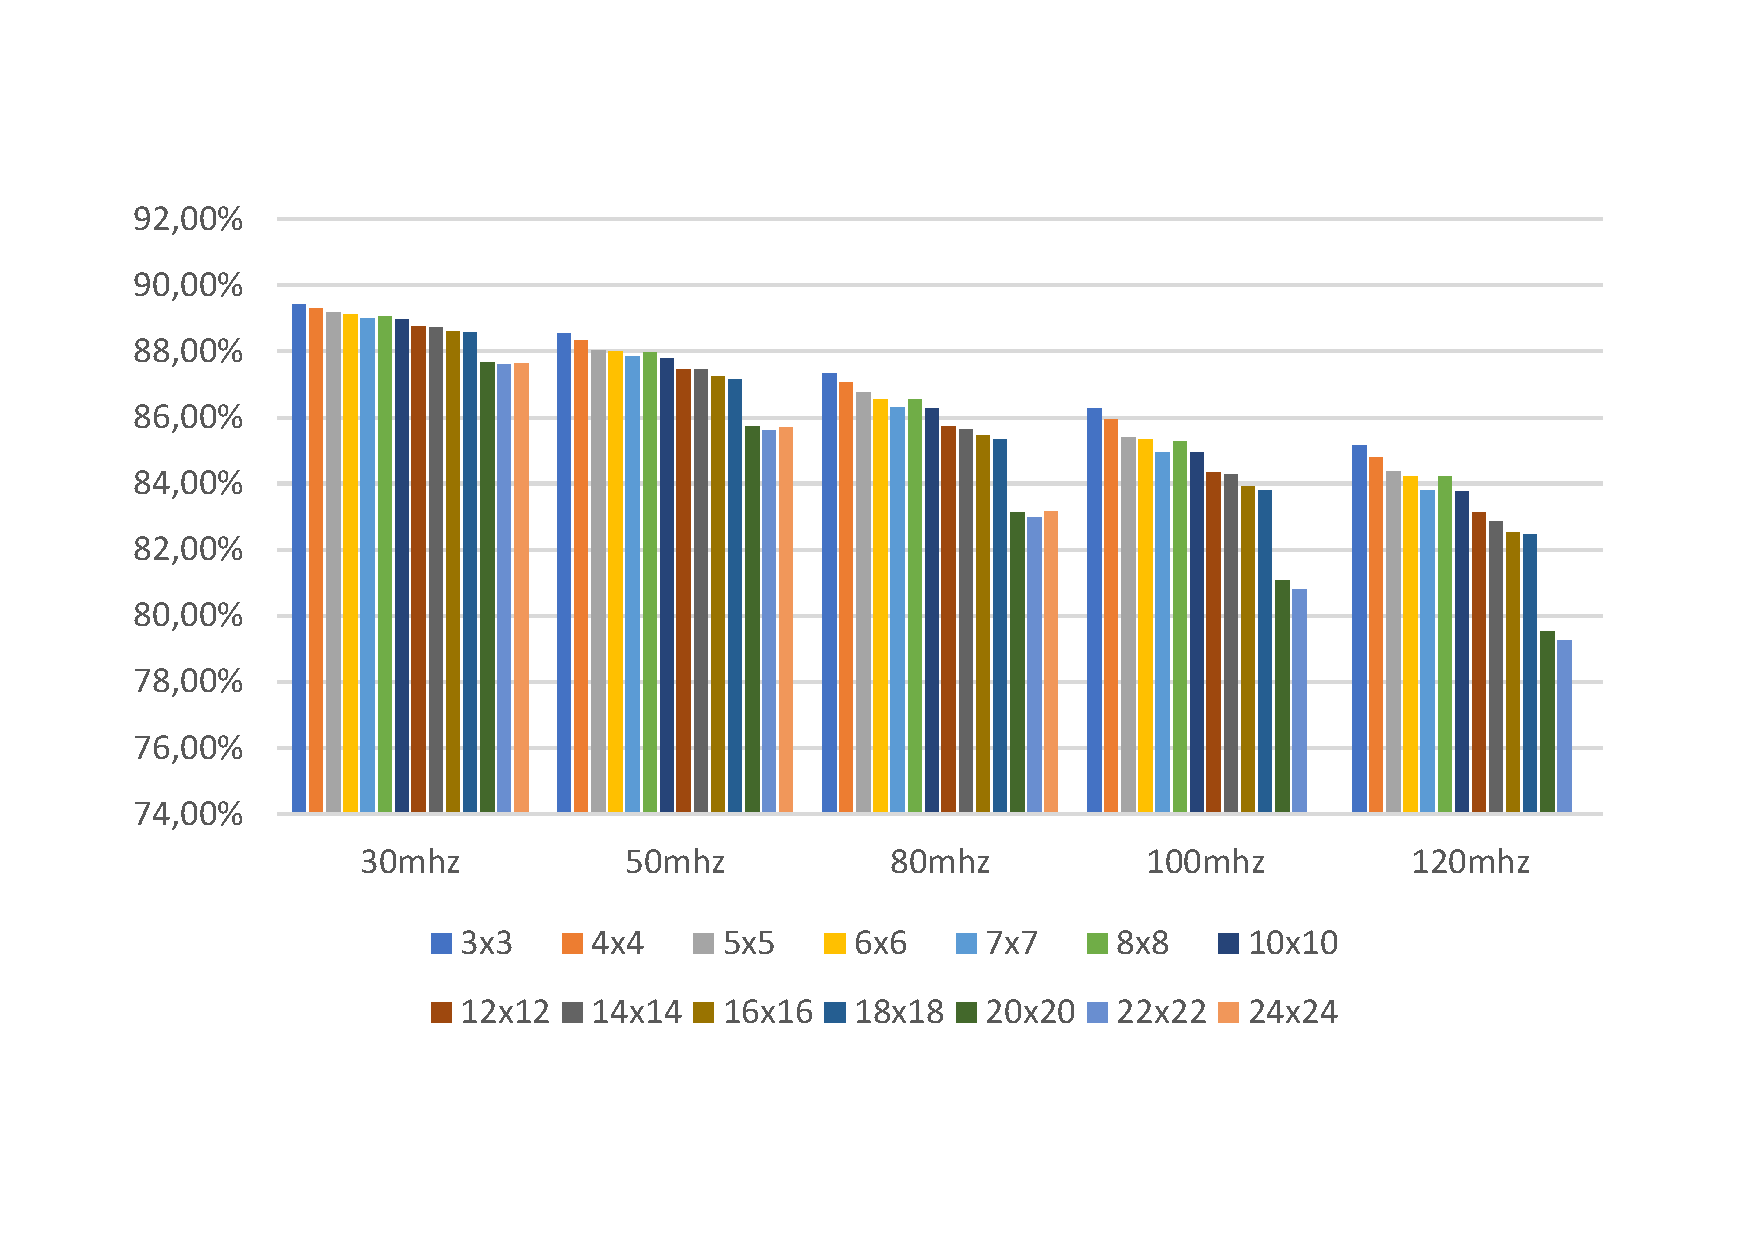
\includegraphics[scale=0.45,angle=0]{./figure/graphs/power_ps_int8_freq.pdf}
\caption{Post Implementation Power Consumption of Processing System for integer 8 PEs}
\label{fig:powint8}
\end{figure}
\begin{figure}[!htbp]
\centering
\captionsetup{justification=centering}
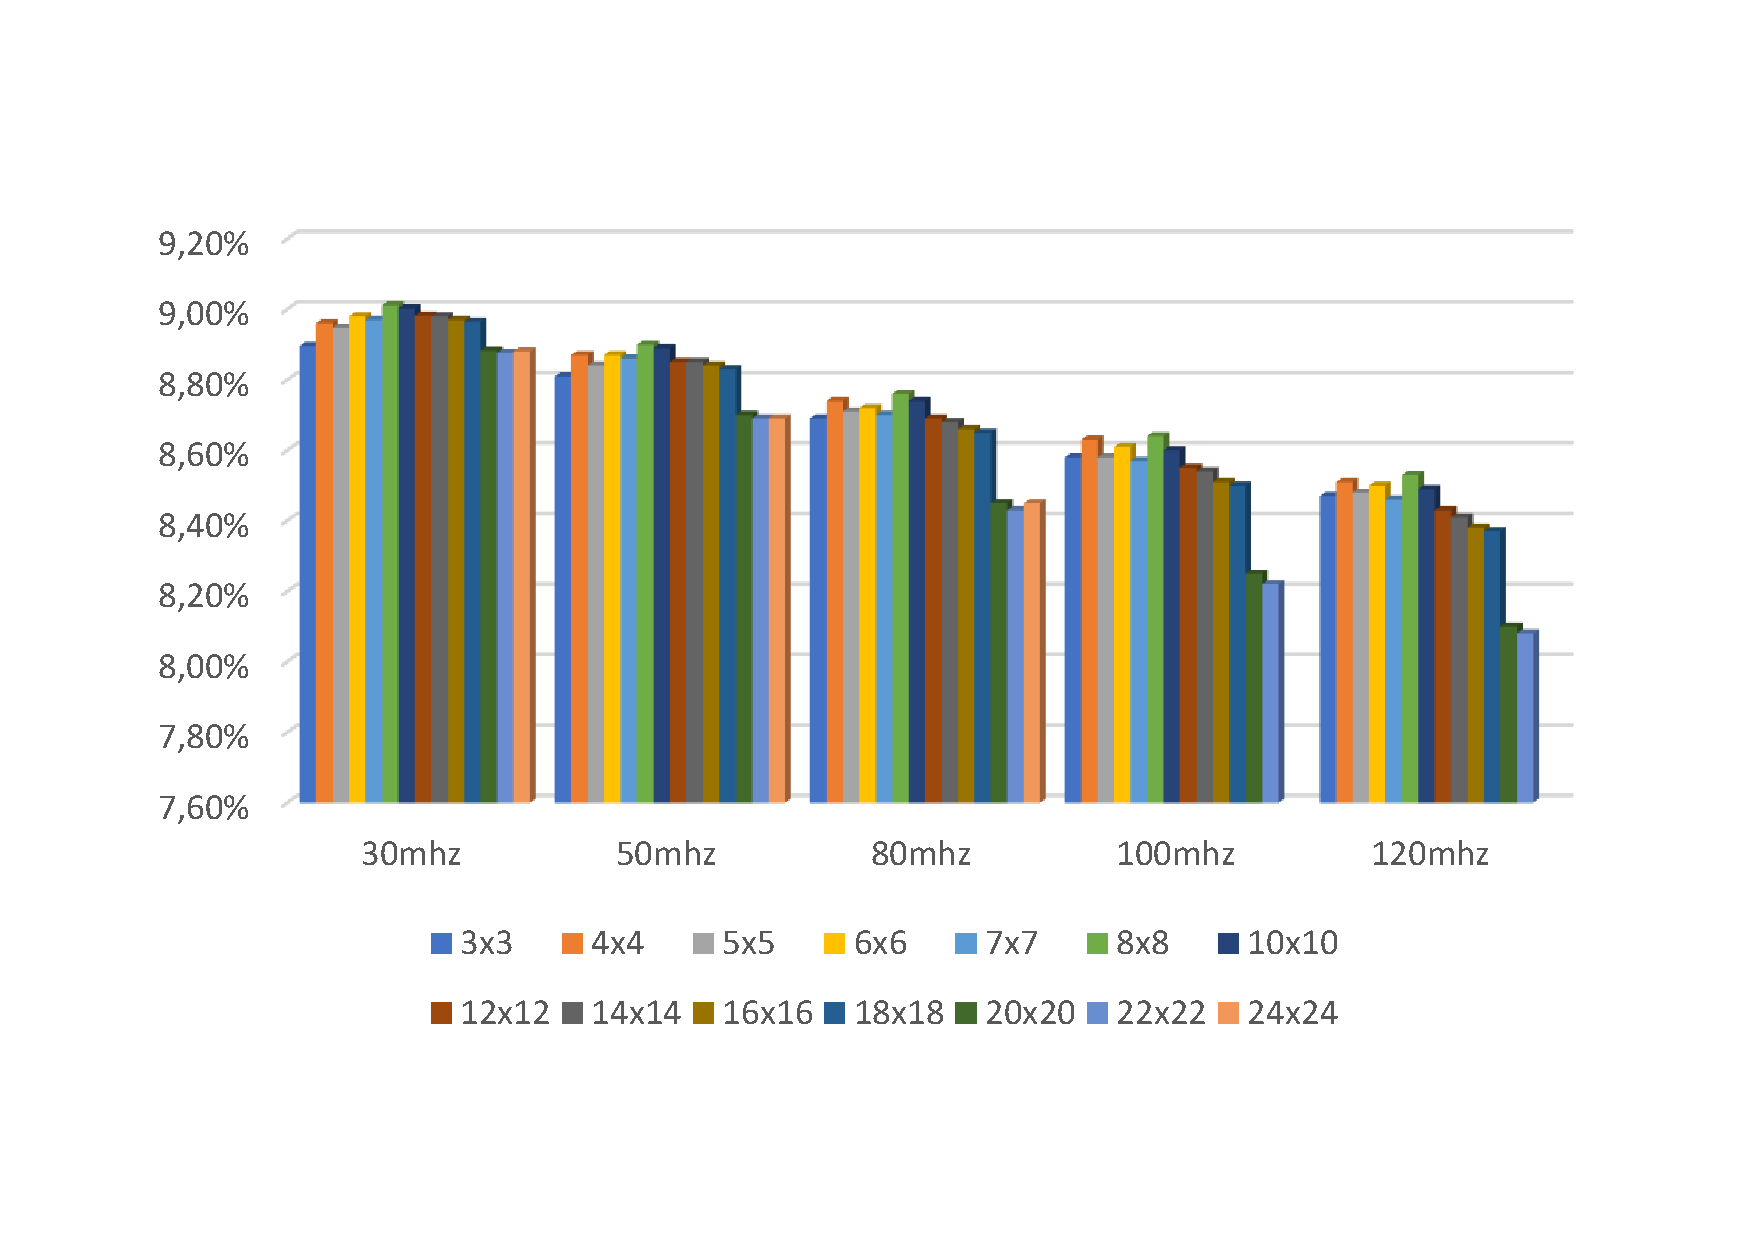
\includegraphics[scale=0.45,angle=0]{./figure/graphs/power_plstatic_int8_freq.pdf}
\caption{Post Implementation Static Power Consumption Programmable logic for integer 8 PEs }
\label{fig:staticpowint8}
\end{figure}
\begin{figure}[!htbp]
\centering
\captionsetup{justification=centering}
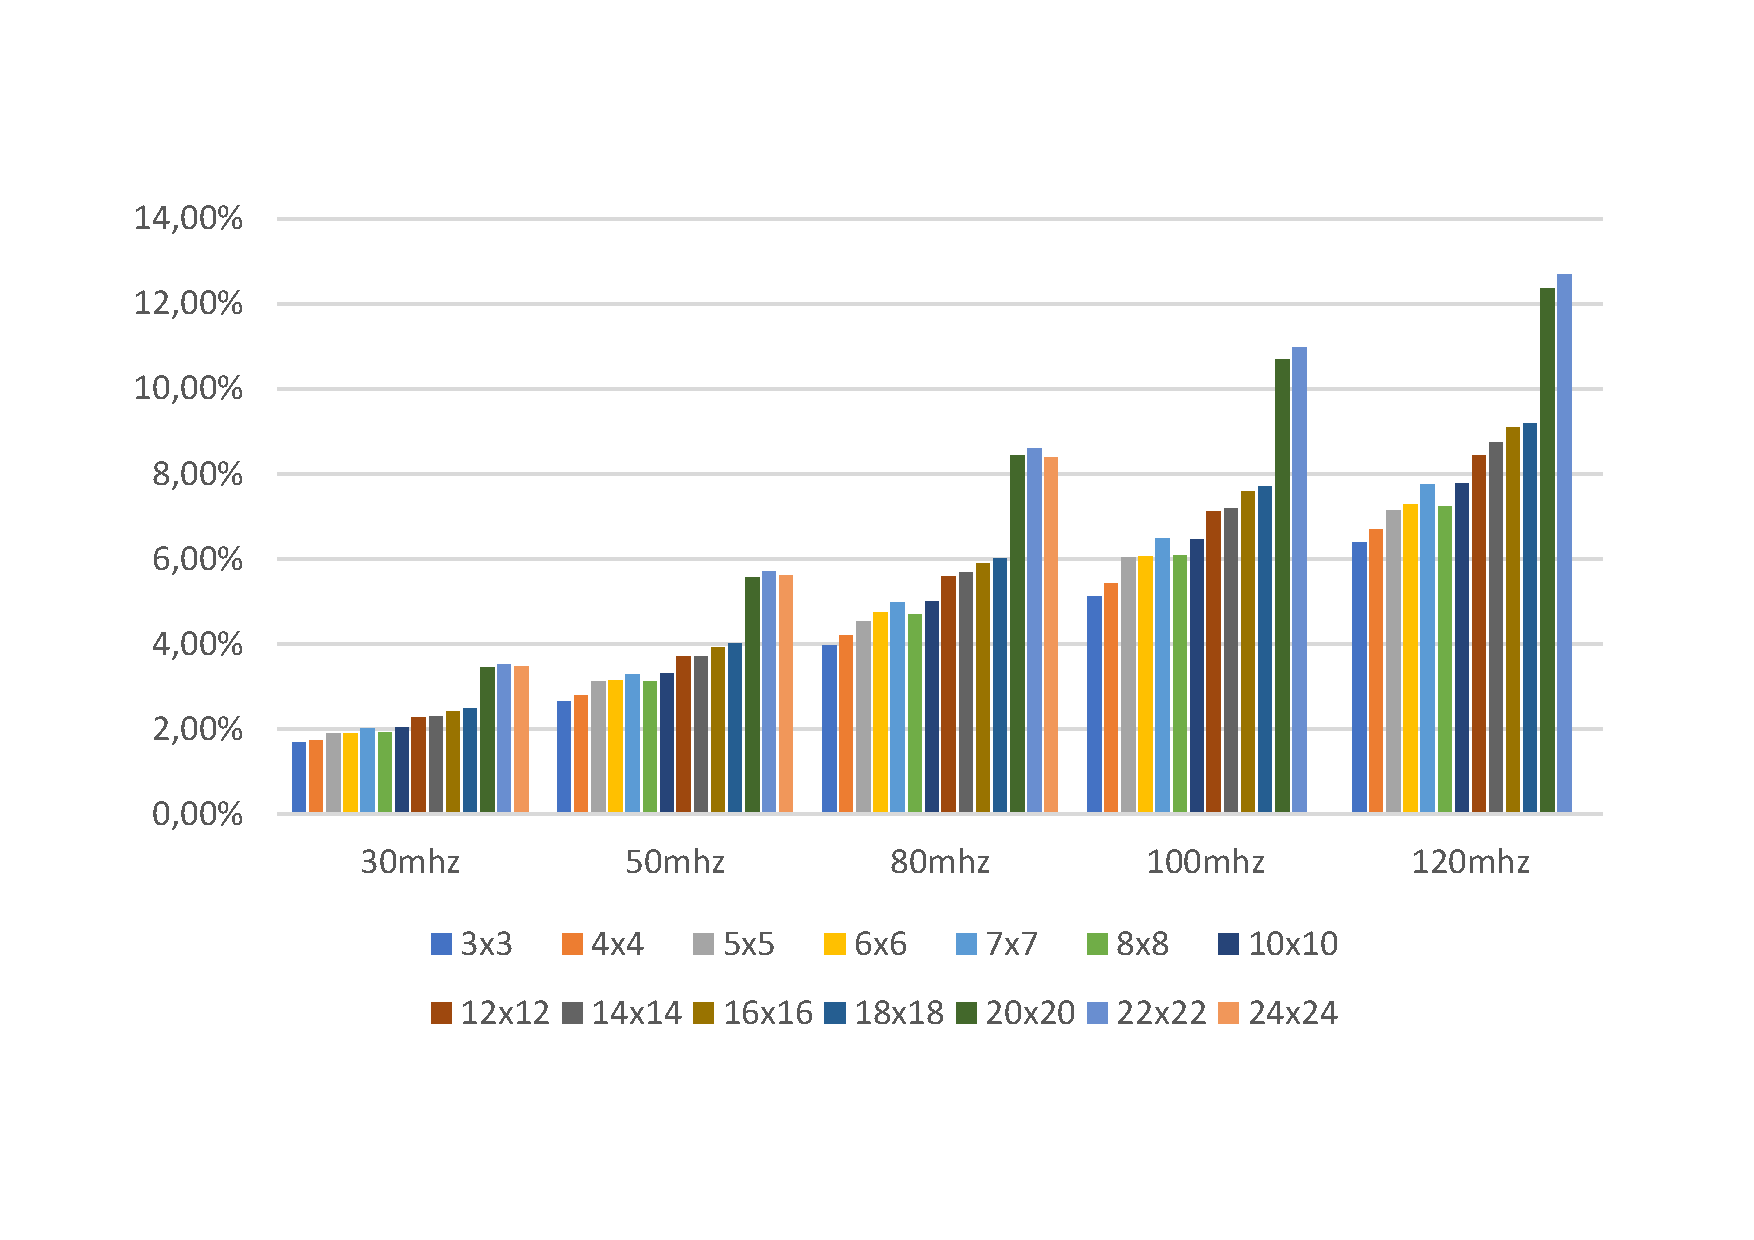
\includegraphics[scale=0.45,angle=0]{./figure/graphs/power_pldyn_int8_freq.pdf}
\caption{Post Implementation Dynamic Power Consumption per Programmable logic with integer 8 PEs}
\label{fig:dynpowint8}
\end{figure}\\\\
The previous Figures represent the behaviour of the power consumption with different Matrix Multiplicatio Unit and for different clock frequency. It is expressed as percentage with reference to the total power consumption of the SoC ( processing system and programmable logic). In fact it can be seen that the power consumption of the processing system and the static power consumption have a less impact on the total power consumption with an increase of the Matrix Multiplication Unit and the frequency. On the other hand, the dynamic power consumption \ref{fig:dynpowint8}, as expected, grows with a growing Matrix Multiplication Unit and the design frequency.\\
In the following Figures, the dynamic power consumption for each entities (in percentage, wrt the dynamic power in Figure \ref{fig:dynpowint8}) in the FPGA is analyzed for different clock frequencies.\\
\begin{figure}[!htbp]
\centering
\captionsetup{justification=centering}
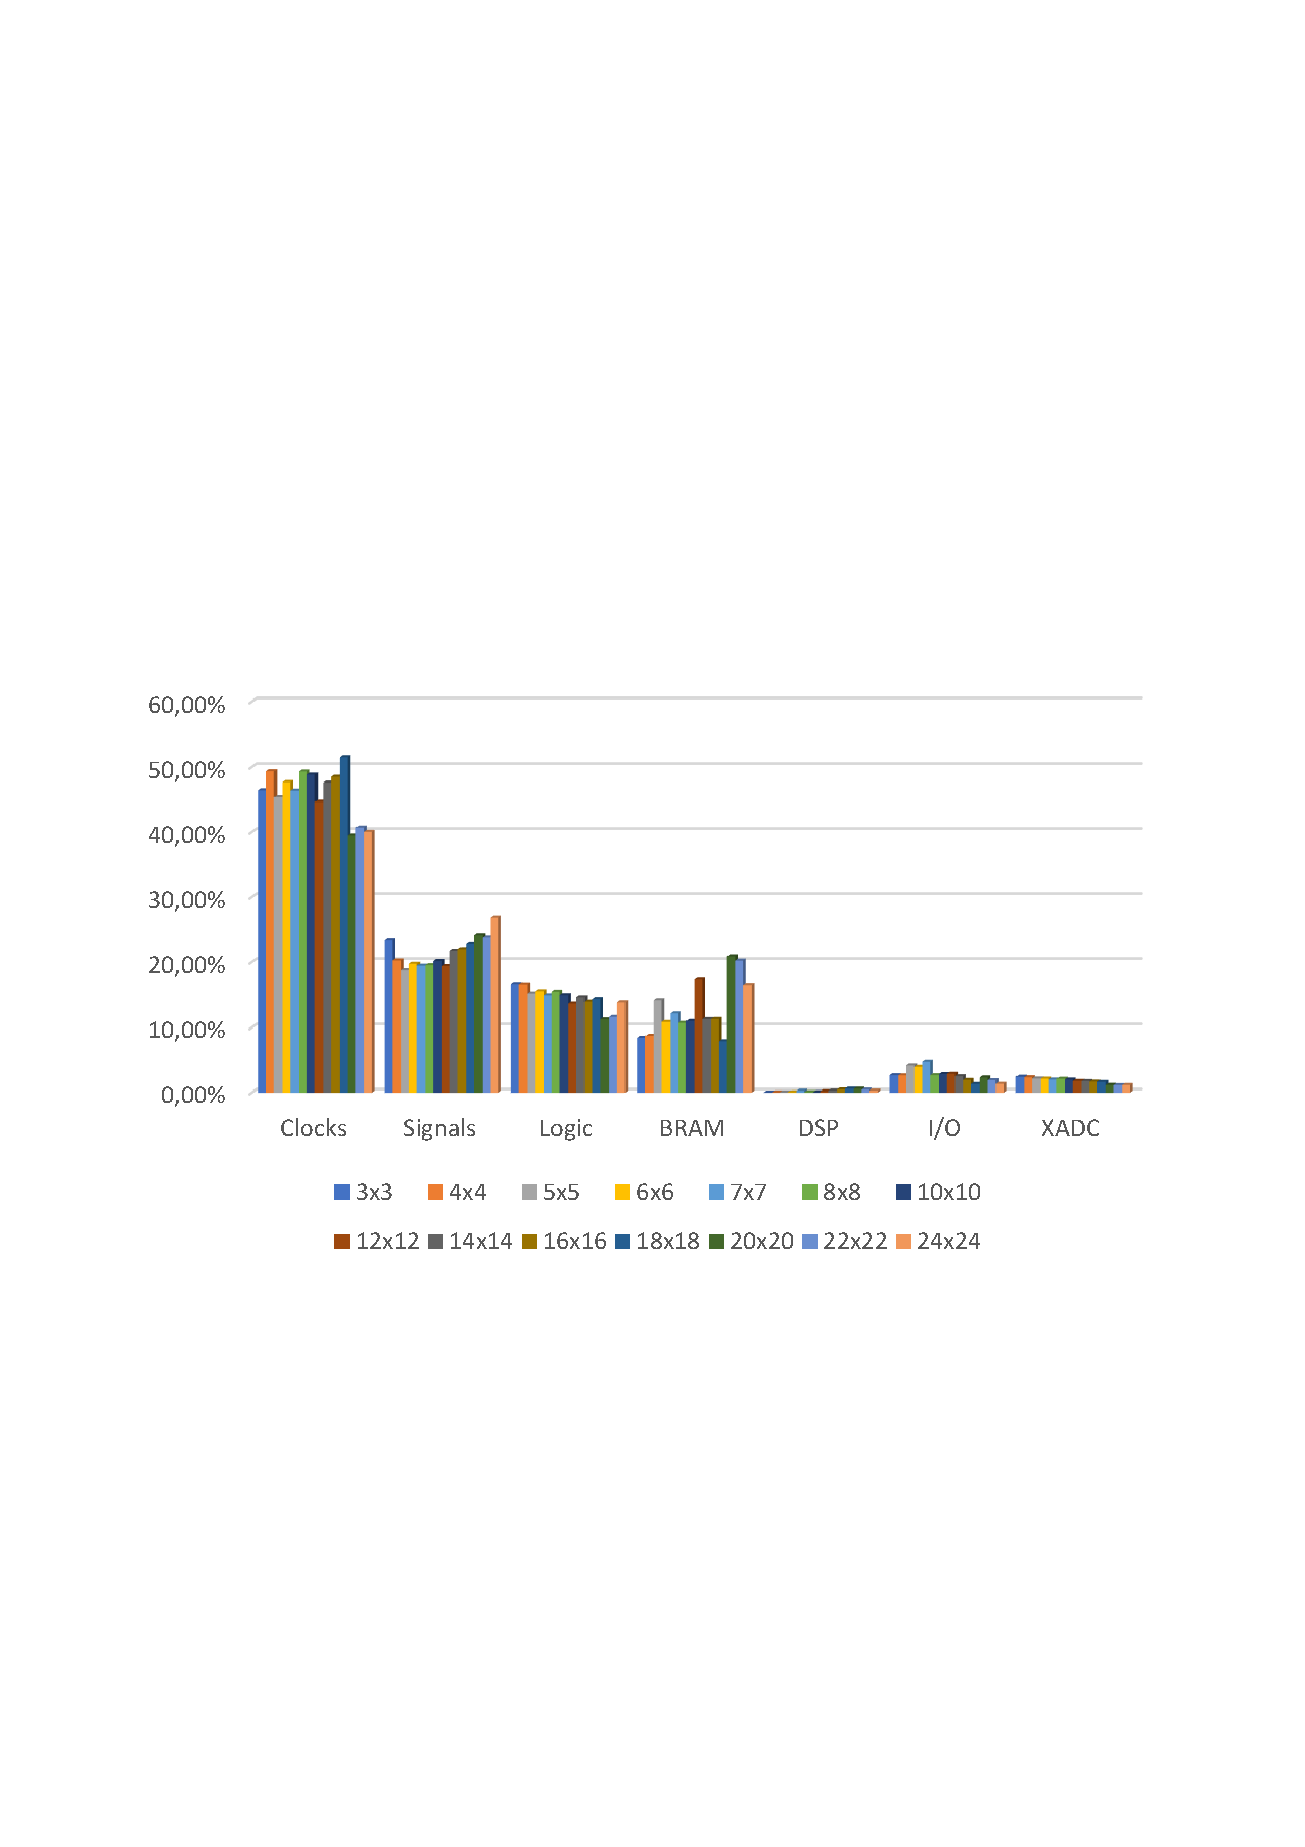
\includegraphics[scale=0.7,angle=0]{./figure/graphs/power_pldyn_div_int8_freq_30mhz.pdf}
\caption{Post Implementation Dynamic Power Consumption per entities in Programmable Logic with a clock frequency of 30 MHz and integer 8 PEs}
\label{fig:dynpowint8ent30}
\end{figure}
\begin{figure}[!htbp]
\centering
\captionsetup{justification=centering}
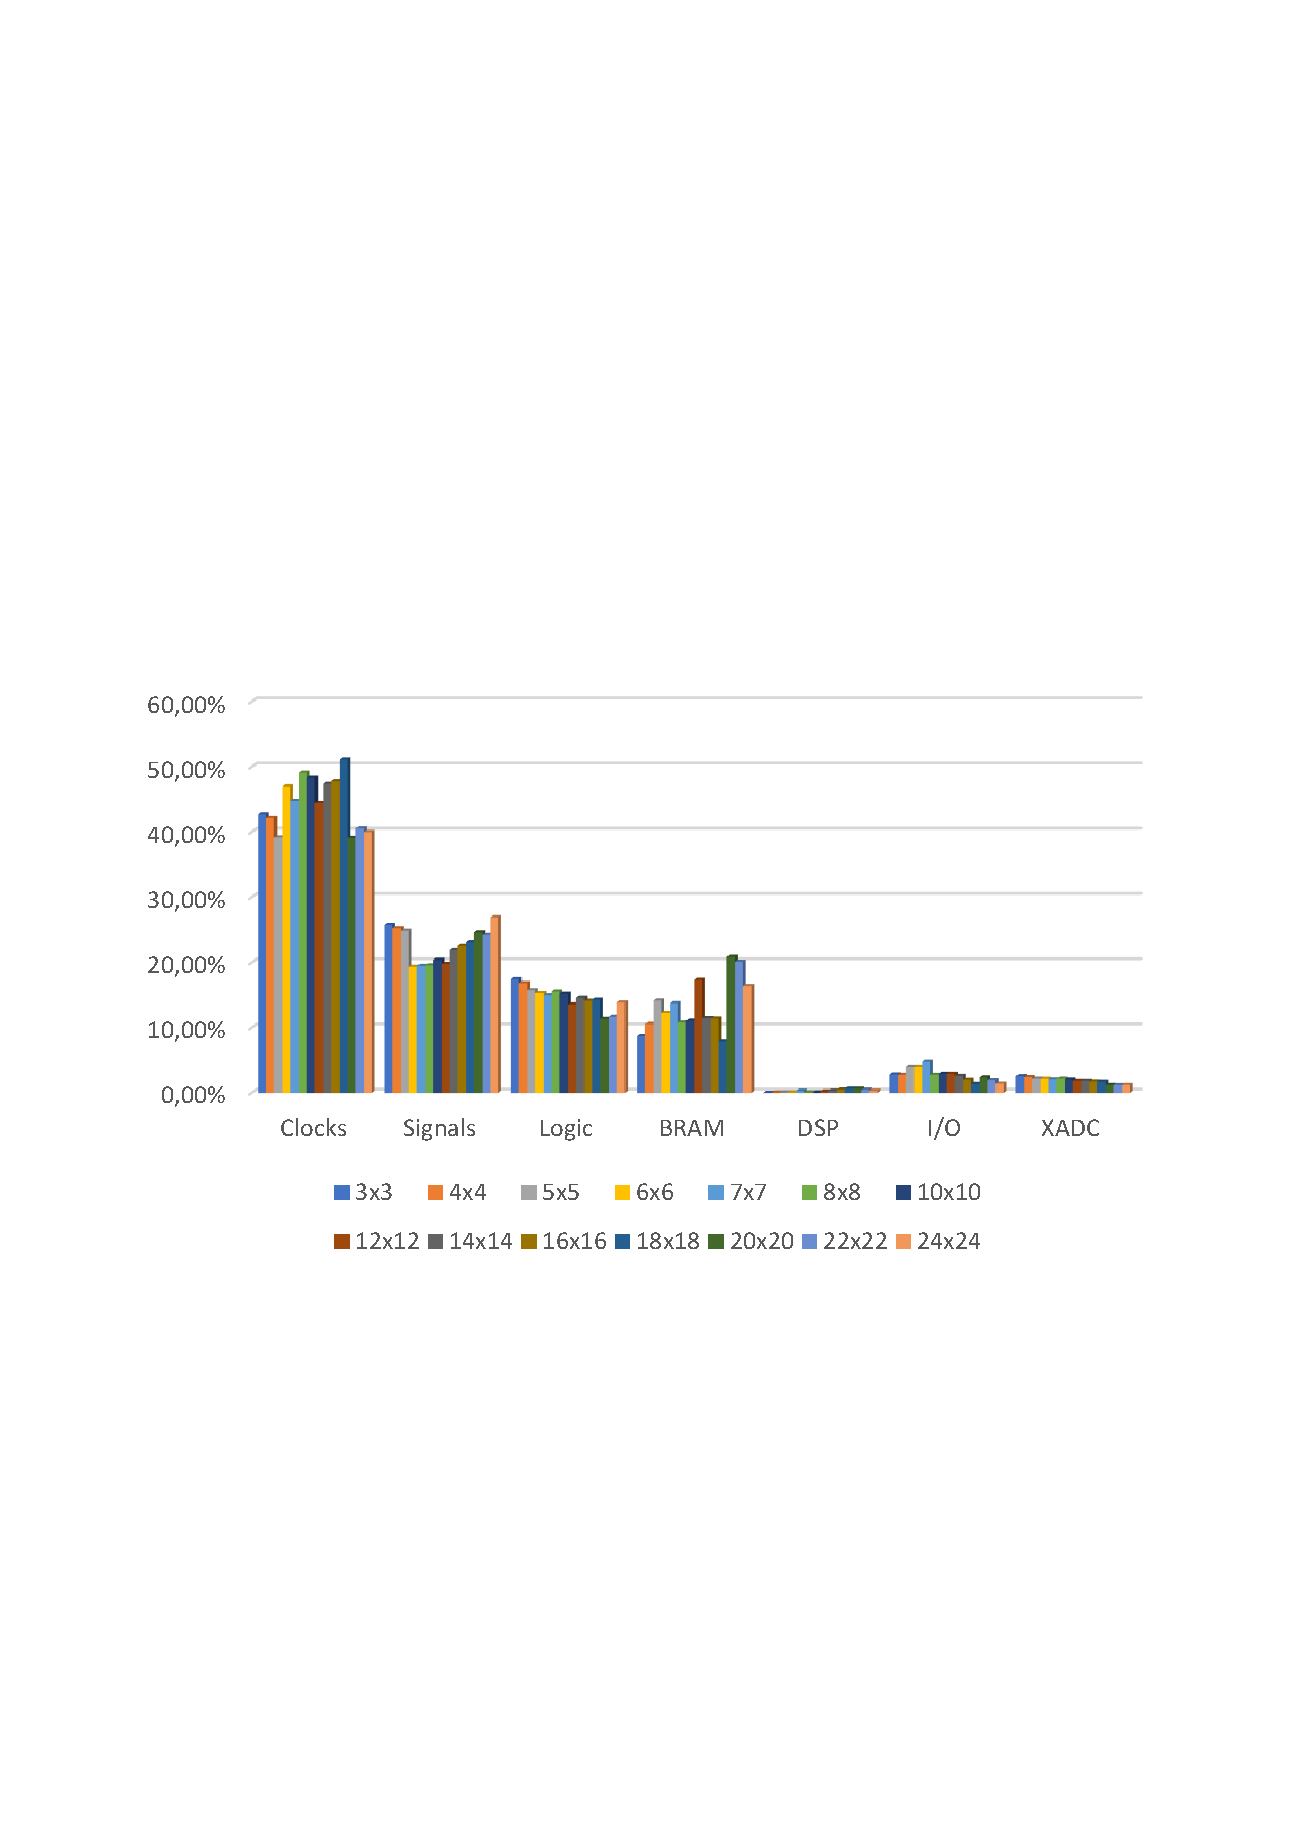
\includegraphics[scale=0.7,angle=0]{./figure/graphs/power_pldyn_div_int8_freq_50mhz.pdf}
\caption{Post Implementation Dynamic Power Consumption per entities in Programmable Logic with a clock frequency of 50 MHz and integer 8 PEs}
\label{fig:dynpowint8ent50}
\end{figure}
\begin{figure}[!htbp]
\centering
\captionsetup{justification=centering}
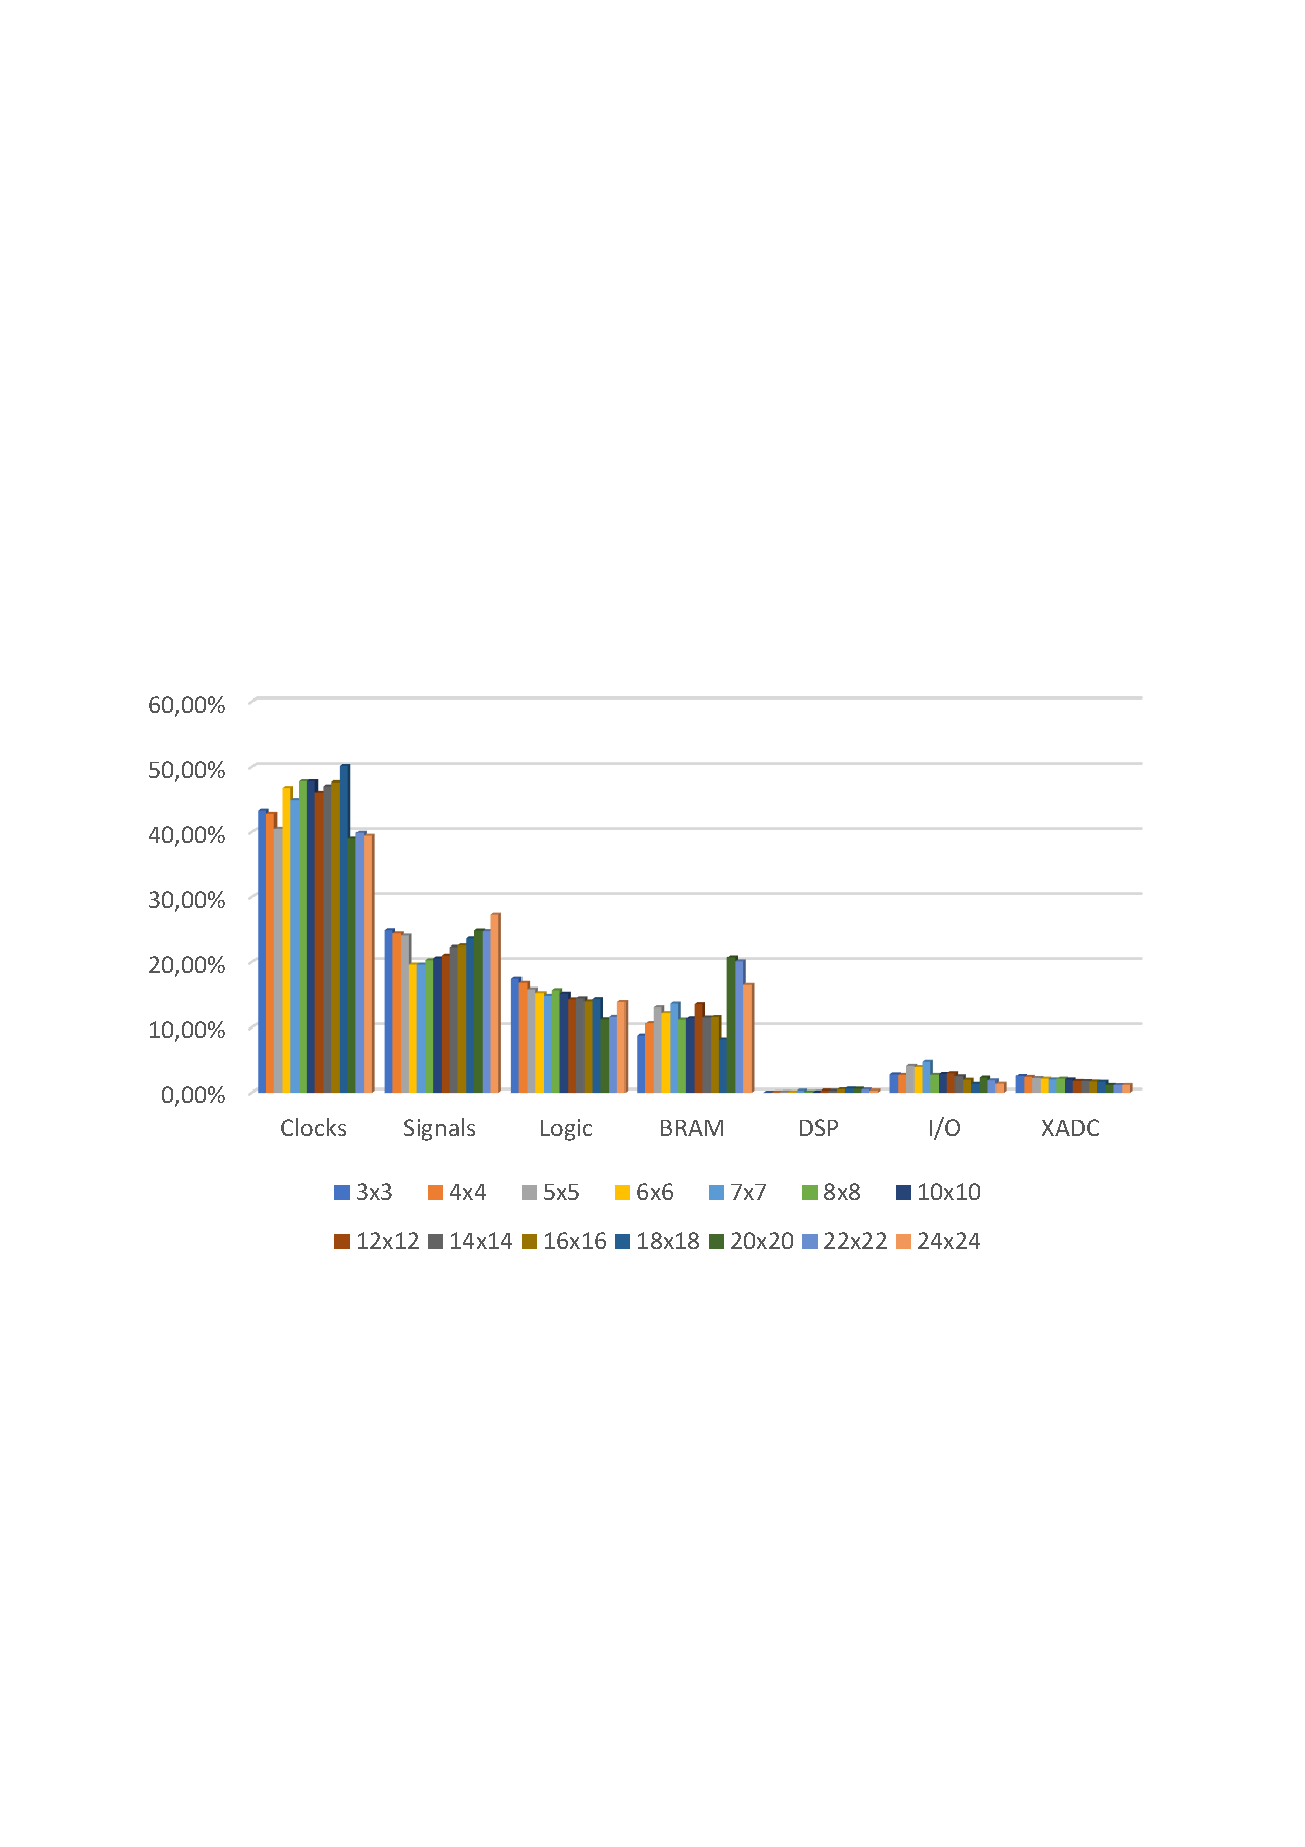
\includegraphics[scale=0.7,angle=0]{./figure/graphs/power_pldyn_div_int8_freq_80mhz.pdf}
\caption{Post Implementation Dynamic Power Consumption per entities in Programmable Logic with a clock frequency of 80 MHz and integer 8 PEs}
\label{fig:dynpowint8ent80}
\end{figure}
\begin{figure}[!htbp]
\centering
\captionsetup{justification=centering}
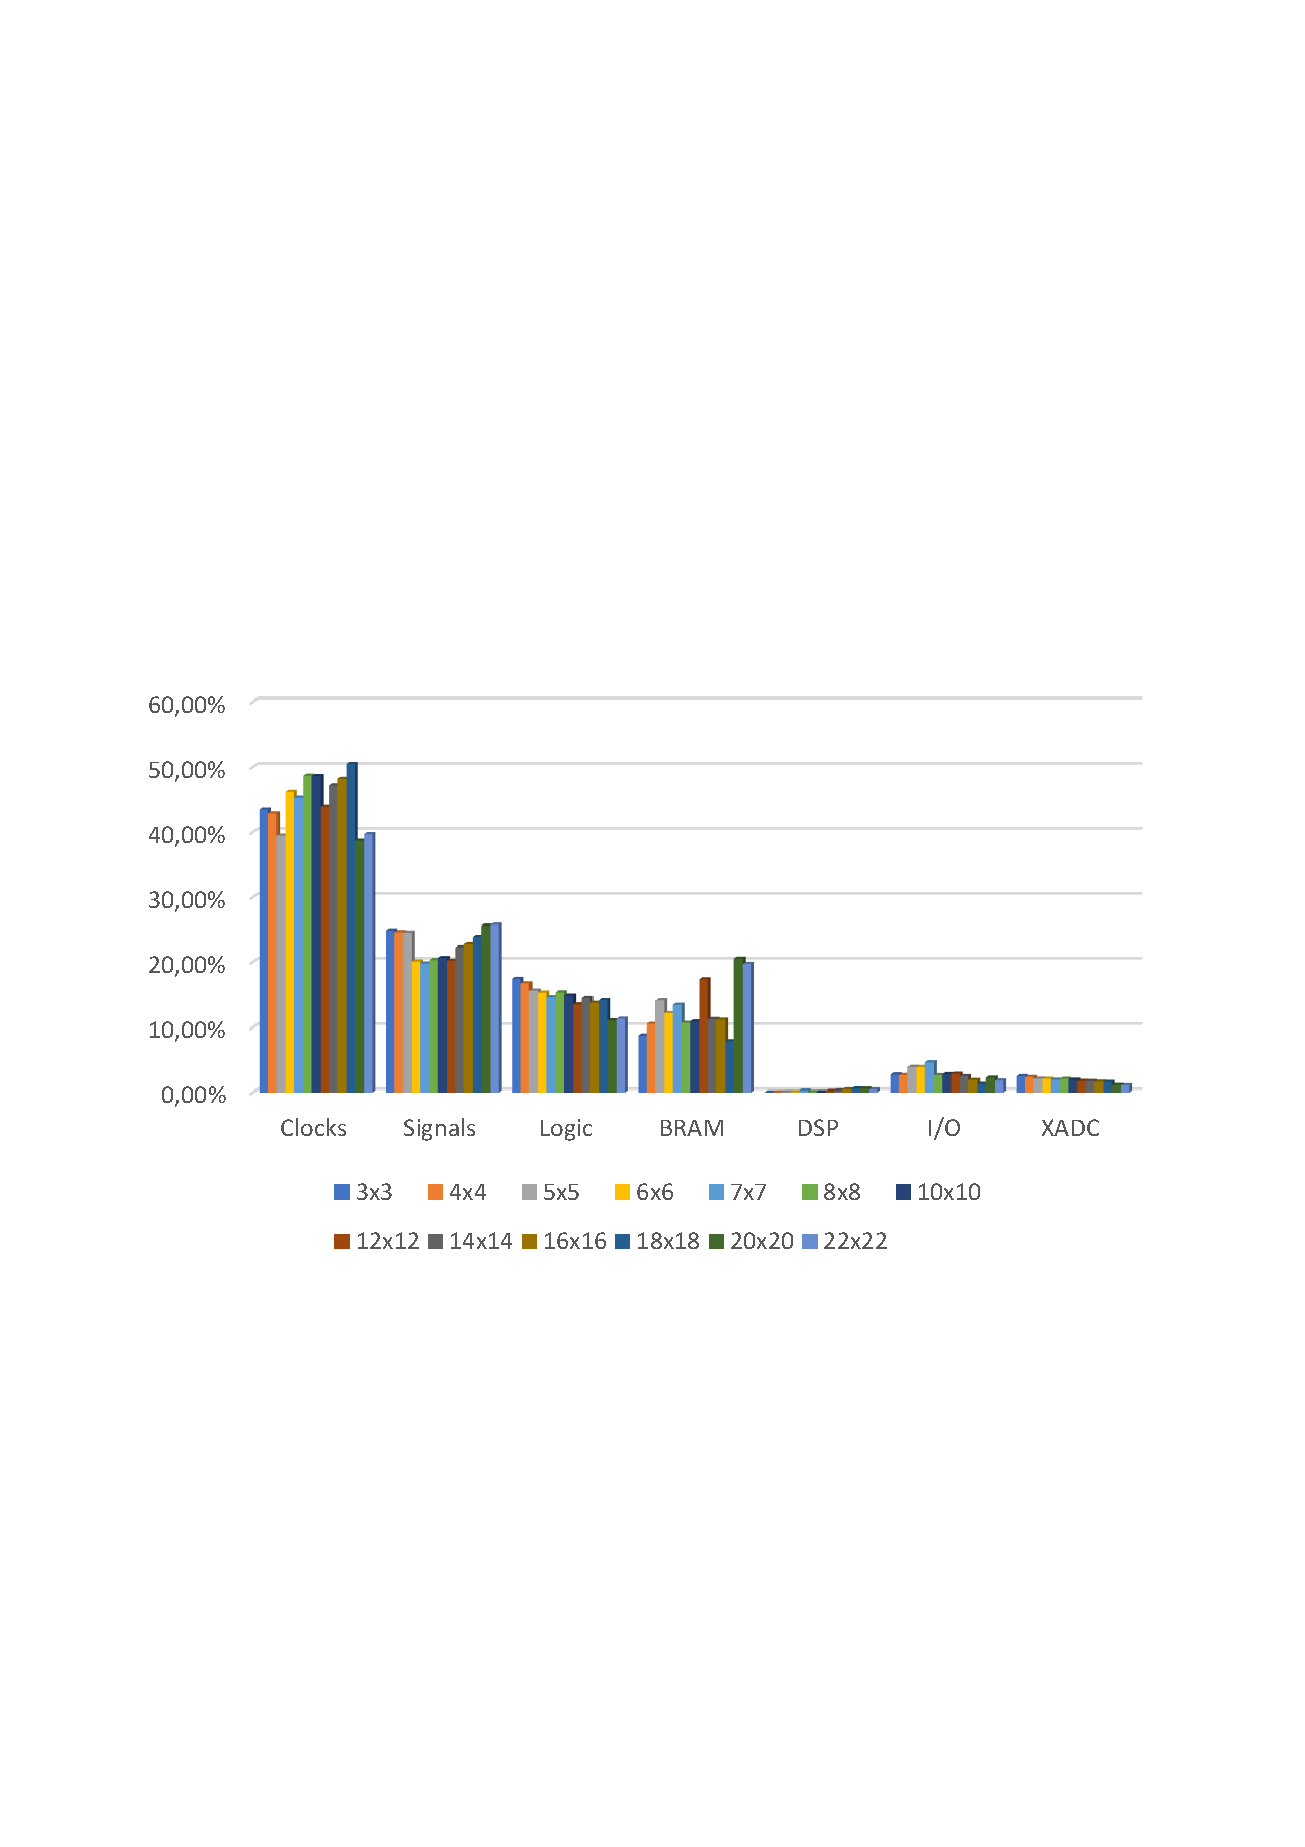
\includegraphics[scale=0.7,angle=0]{./figure/graphs/power_pldyn_div_int8_freq_100mhz.pdf}
\caption{Post Implementation Dynamic Power Consumption per entities in Programmable Logic with a clock frequency of 100 MHz and integer 8 PEs}
\label{fig:dynpowint8ent100}
\end{figure}
\begin{figure}[!htbp]
\centering
\captionsetup{justification=centering}
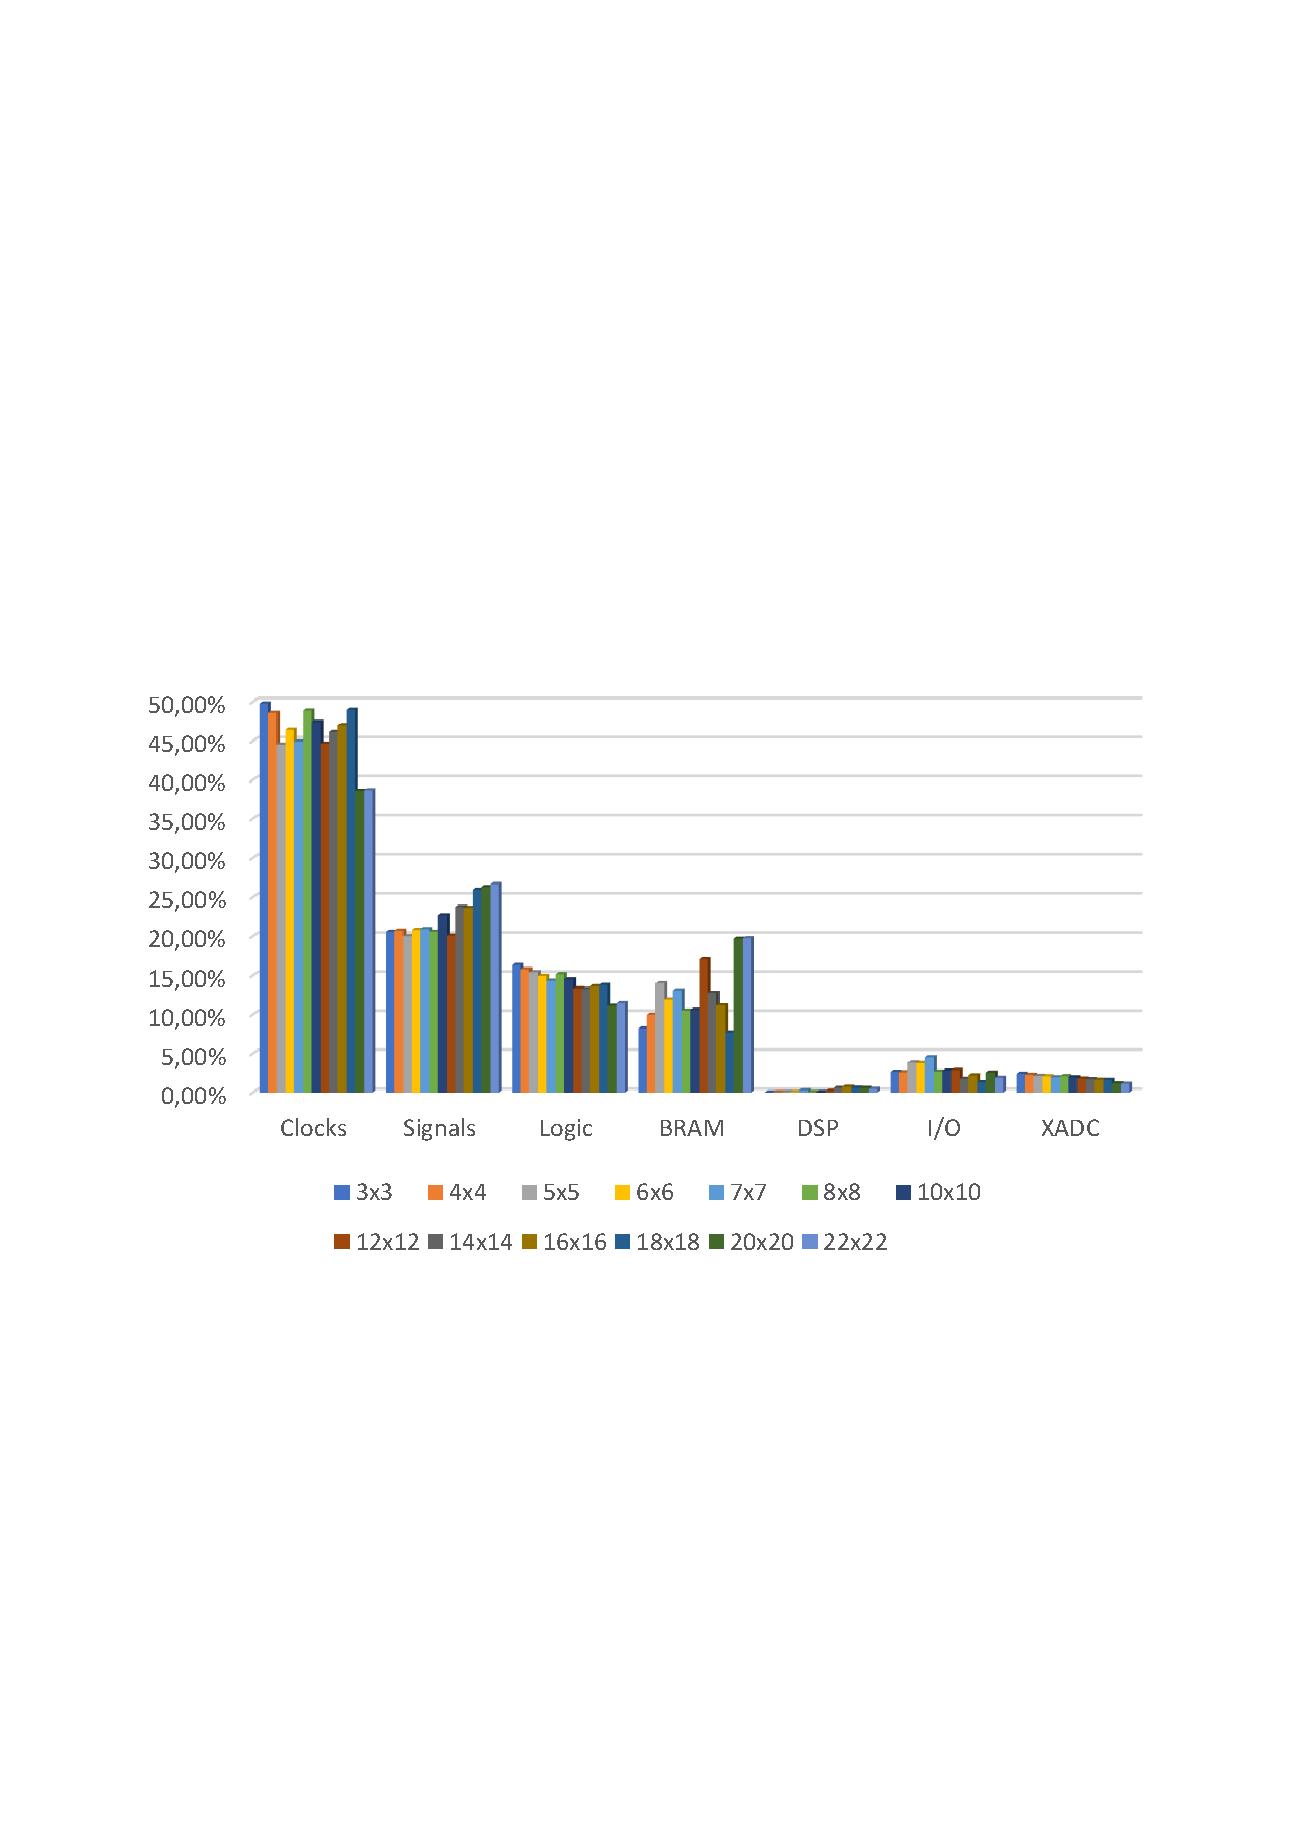
\includegraphics[scale=0.7,angle=0]{./figure/graphs/power_pldyn_div_int8_freq_120mhz.pdf}
\caption{Post Implementation Dynamic Power Consumption per entities in Programmable Logic with a clock frequency of 120 MHz and integer 8 PEs}
\label{fig:dynpowint8ent120}
\end{figure}\\\\
As it is very well known, the clock distribution is one of the main source of power consumption, and it is confirmed from all the previos Figures. Also the interconnections, called \textit{signals} in the figures, are power hungry (a bigger MXU leads to many, and longer, interconnections between PEs). In fact the clock distribution networks and the interconnections are the predominant entities of the dynamic power consumption of the programmable logic.
The logic entity is containing all the power consumed by the FFs and LUTs, it looks like their power consumption is decreasing but it is only the percentage of the total dynamic power which is decreasing.
It is worth to mention that the PEs (at least the majority of them) are implemented using the DSP entities. However, the power consumed by those entities is almost negligible,  the DSPs are low power entities in the FGPA according to its datasheet \cite{paper:42}.\\
Regarding the BRAM, I/O and XADC, with an increase or a decrease of the other entities impact they have a slightly modification of their impact on the power consumption.\\
\item Integer 16:\\
In the follwing Figures, the same considerations for the Integer 8 are still valid since the PEs are always implemented on the same DSP entity but without the higher 8 bits of the input values gated to zeros.
\begin{figure}[!htbp]
\centering
\captionsetup{justification=centering}
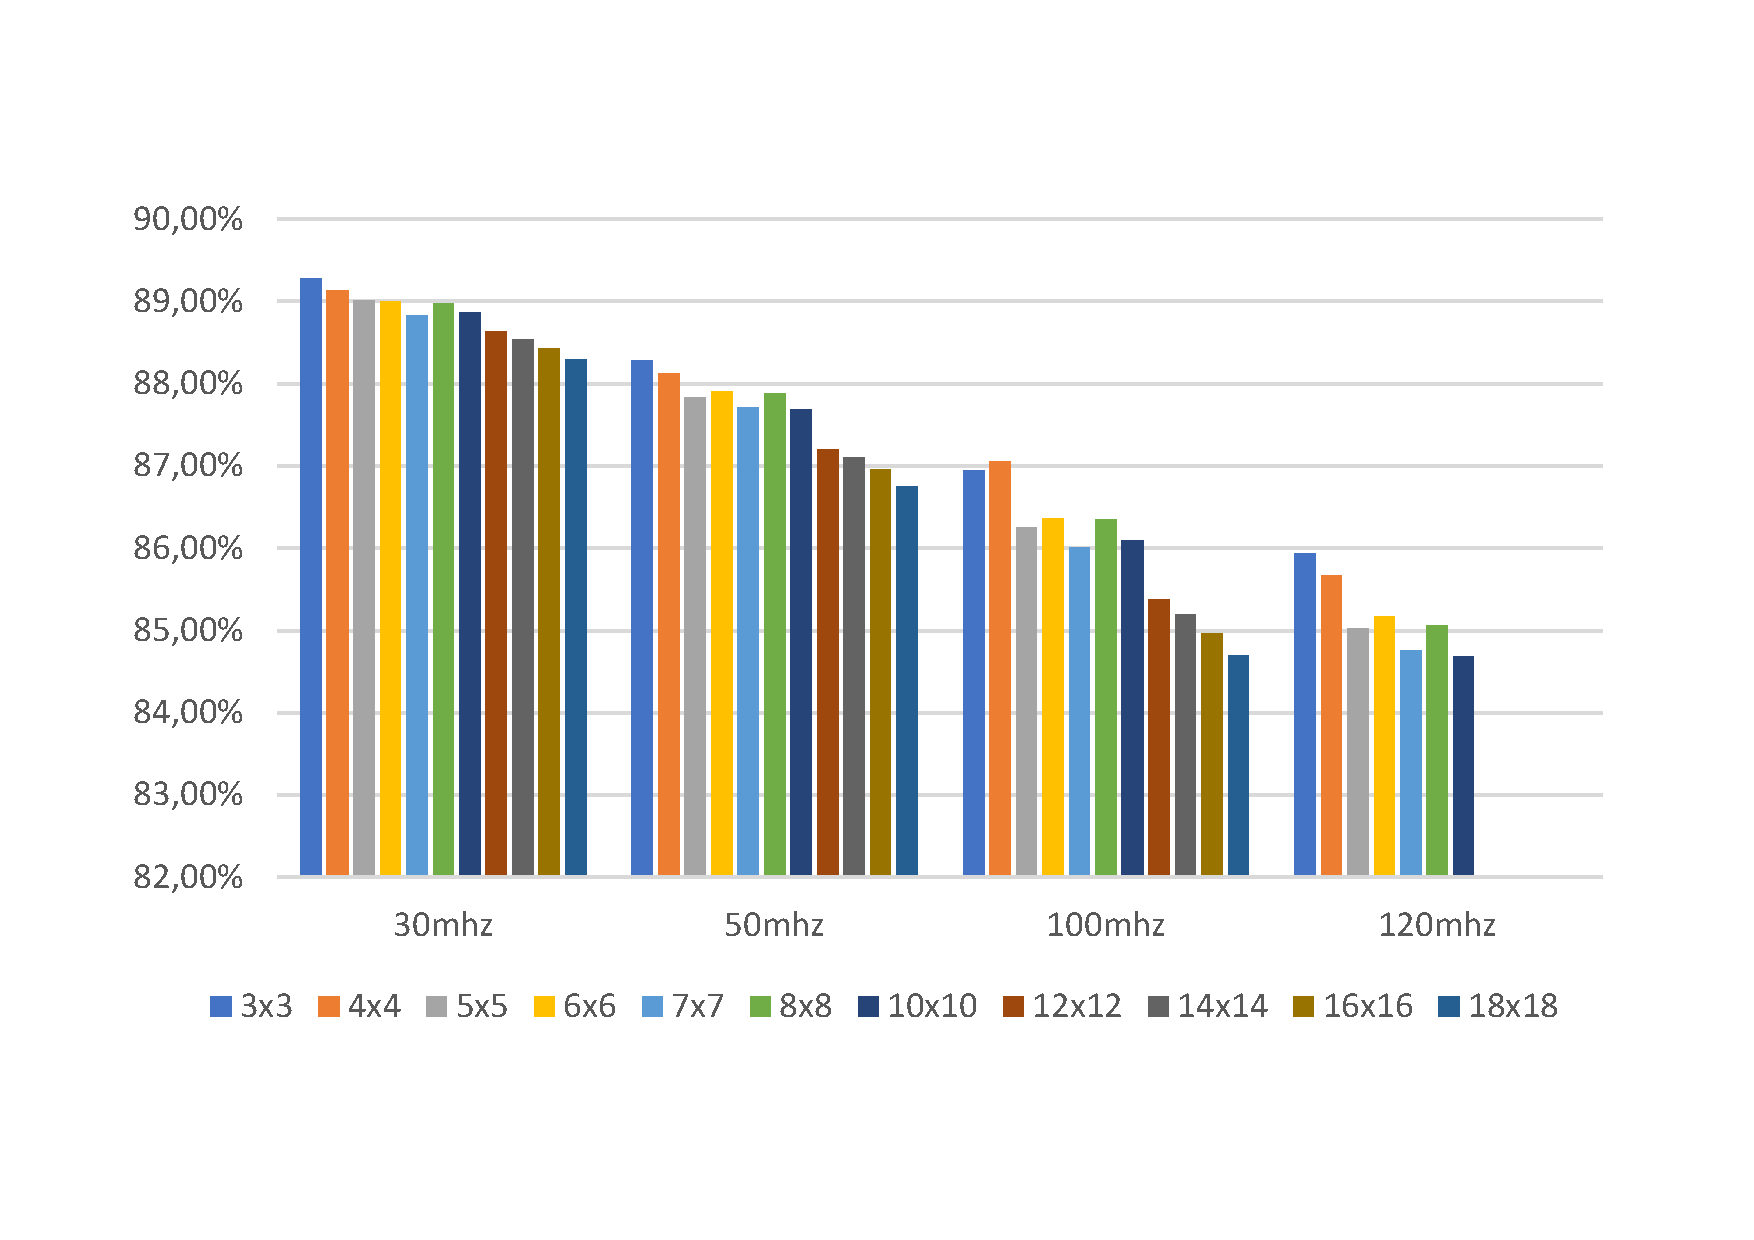
\includegraphics[scale=0.5,angle=0]{./figure/graphs/power_ps_int16_freq.pdf}
\caption{Post Implementation Power Consumption of Processing System for integer 16 PEs}
\label{fig:powint16}
\end{figure}
\begin{figure}[!htbp]
\centering
\captionsetup{justification=centering}
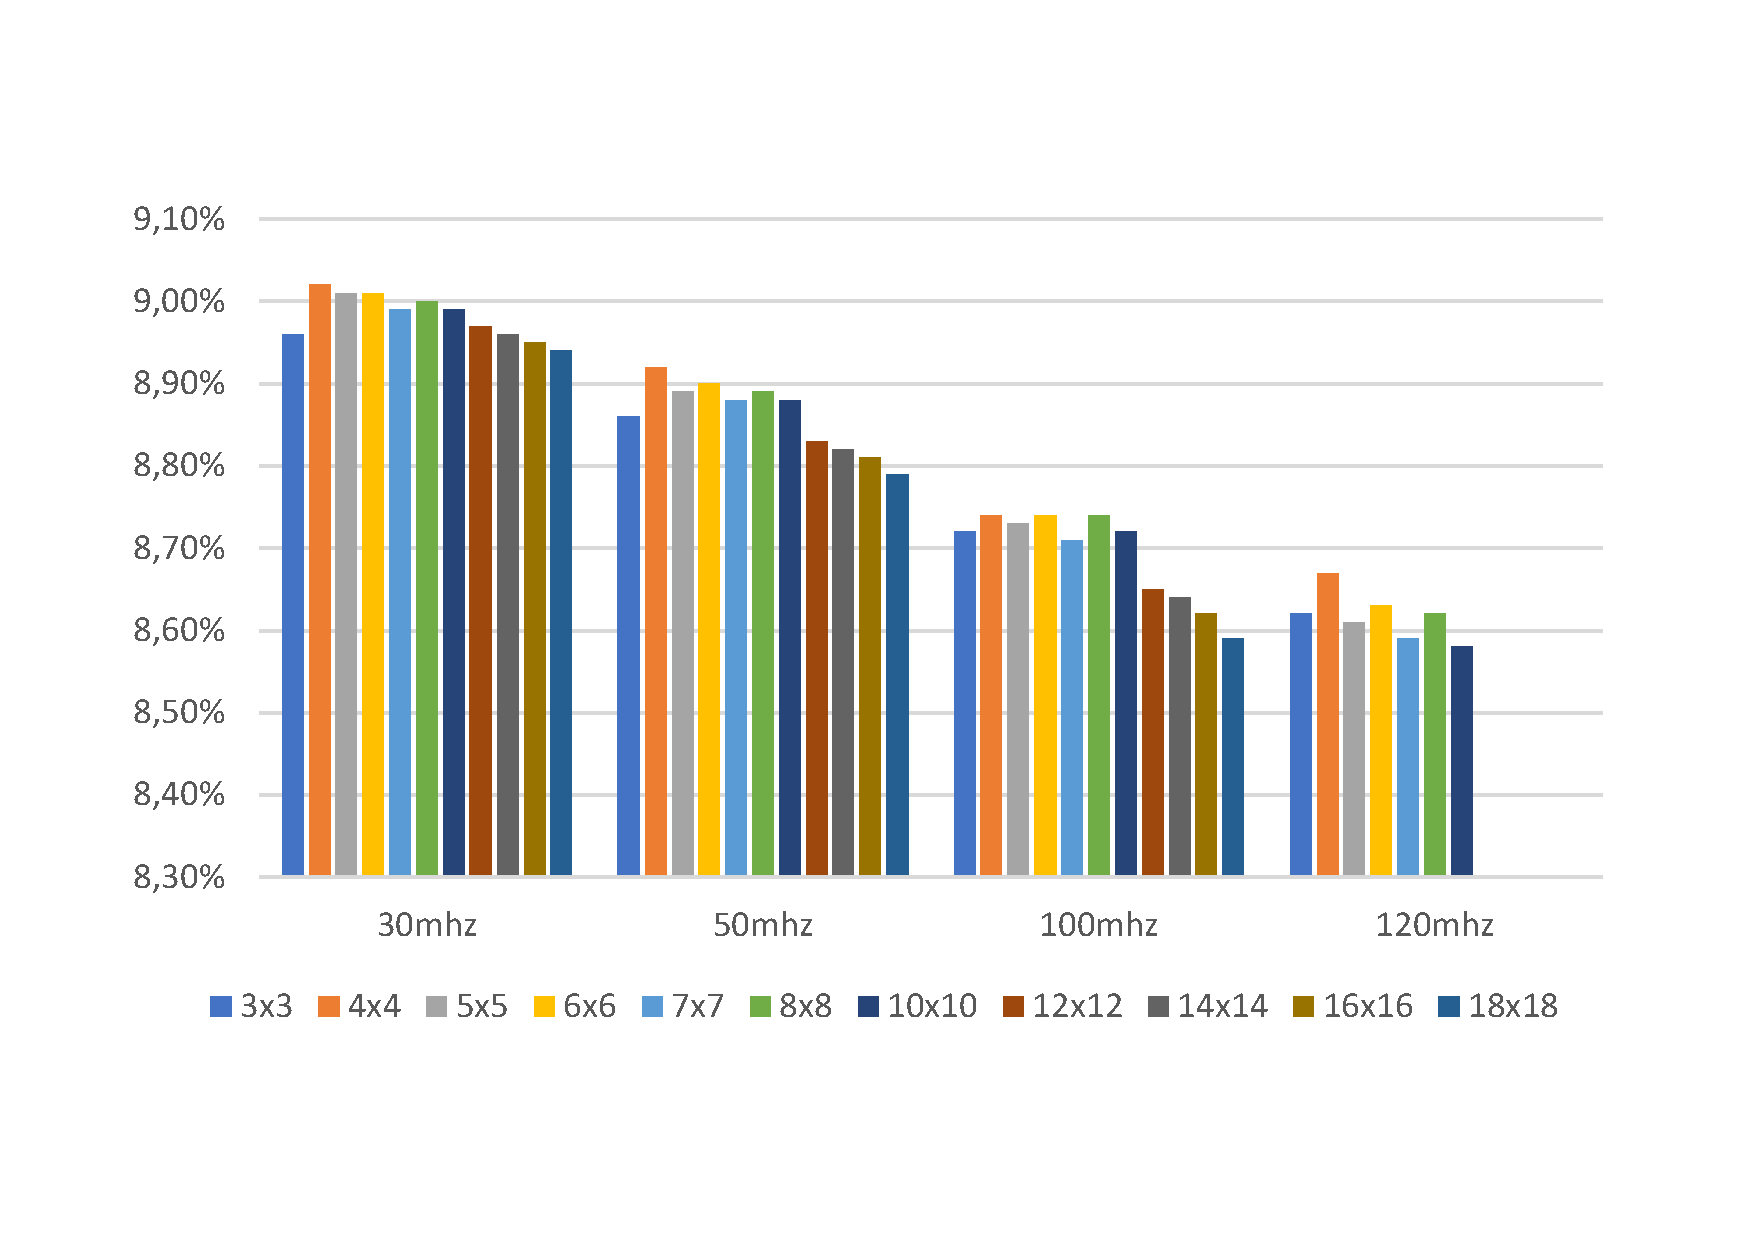
\includegraphics[scale=0.5,angle=0]{./figure/graphs/power_plstatic_int16_freq.pdf}
\caption{Post Implementation Static Power Consumption Programmable logic for integer 16 PEs }
\label{fig:staticpowint16}
\end{figure}
\begin{figure}[!htbp]
\centering
\captionsetup{justification=centering}
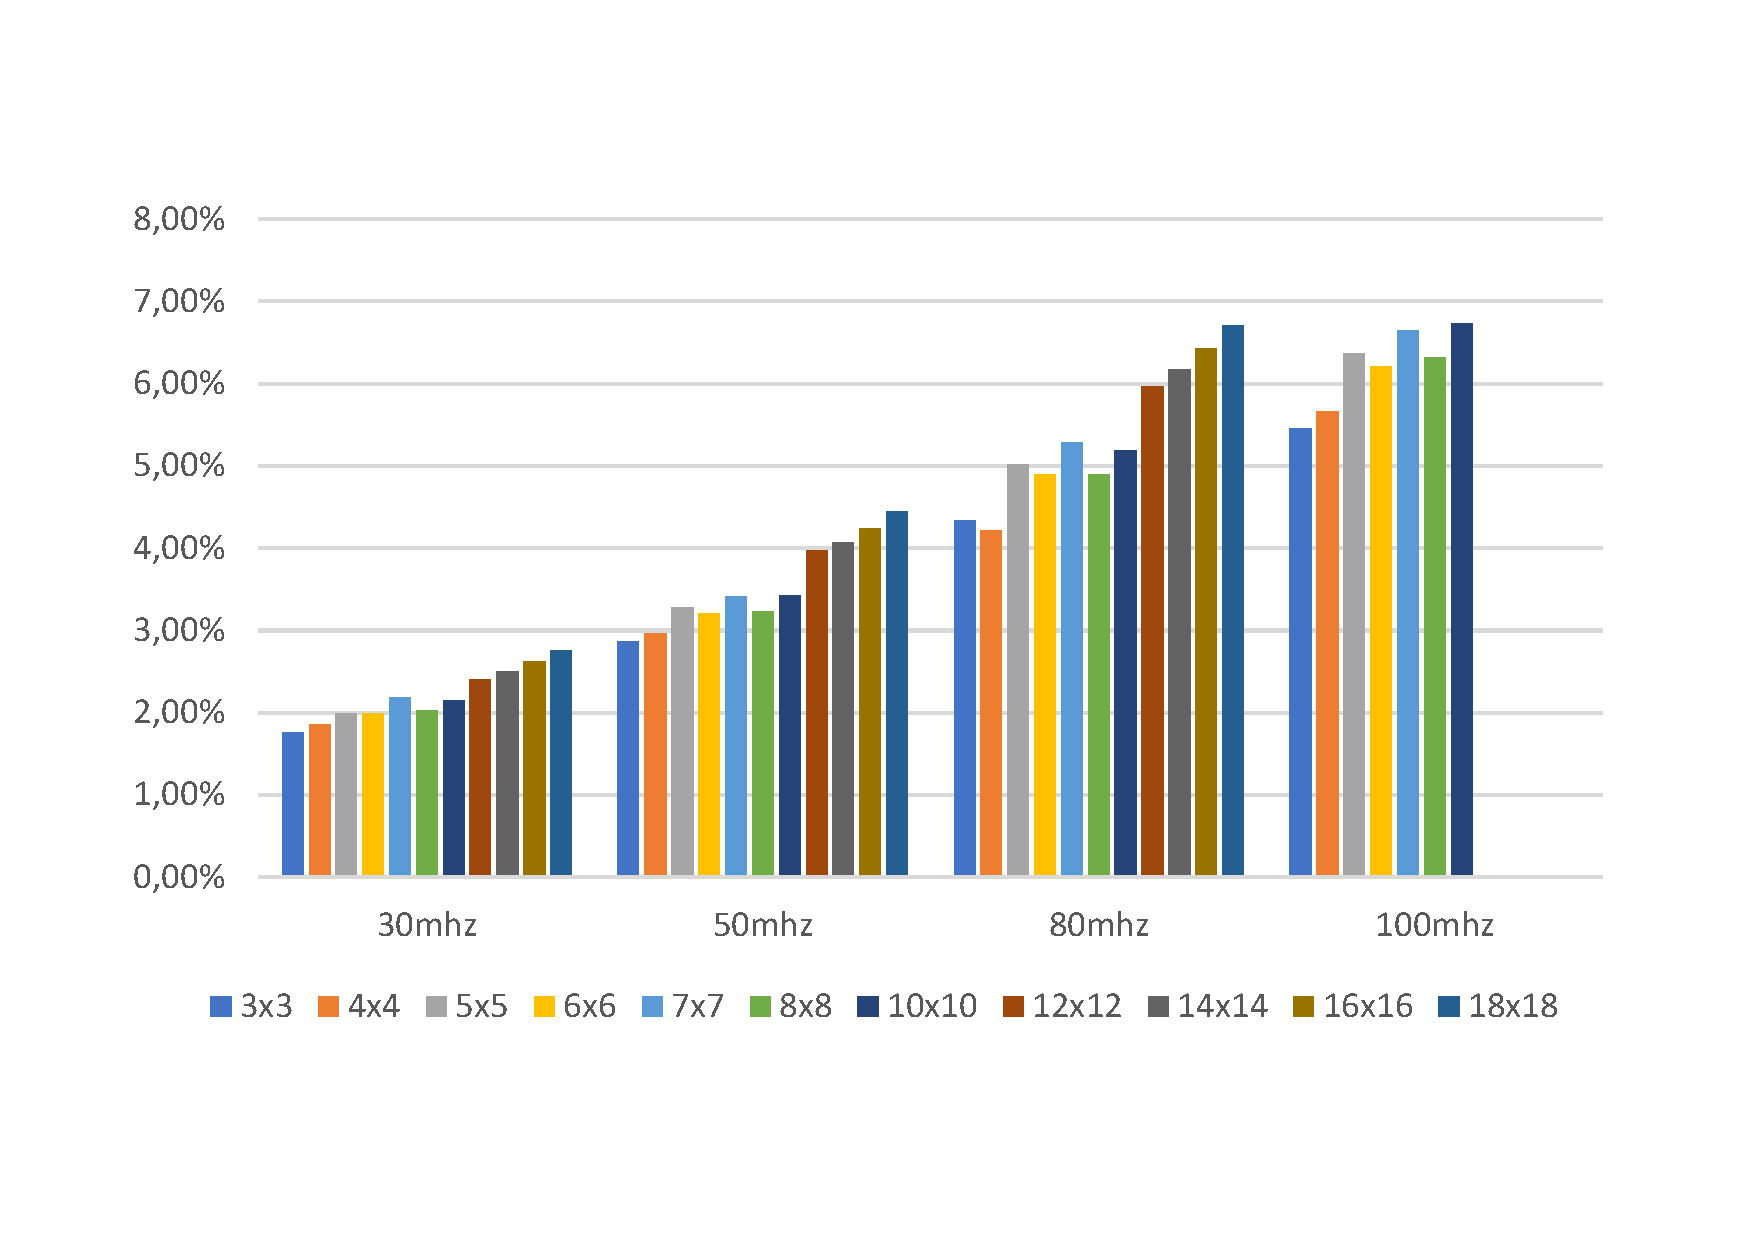
\includegraphics[scale=0.5,angle=0]{./figure/graphs/power_pldyn_int16_freq.pdf}
\caption{Post Implementation Dynamic Power Consumption per Programmable logic with integer 16 PEs}
\label{fig:dynpowint16}
\end{figure}
\begin{figure}[!htbp]
\centering
\captionsetup{justification=centering}
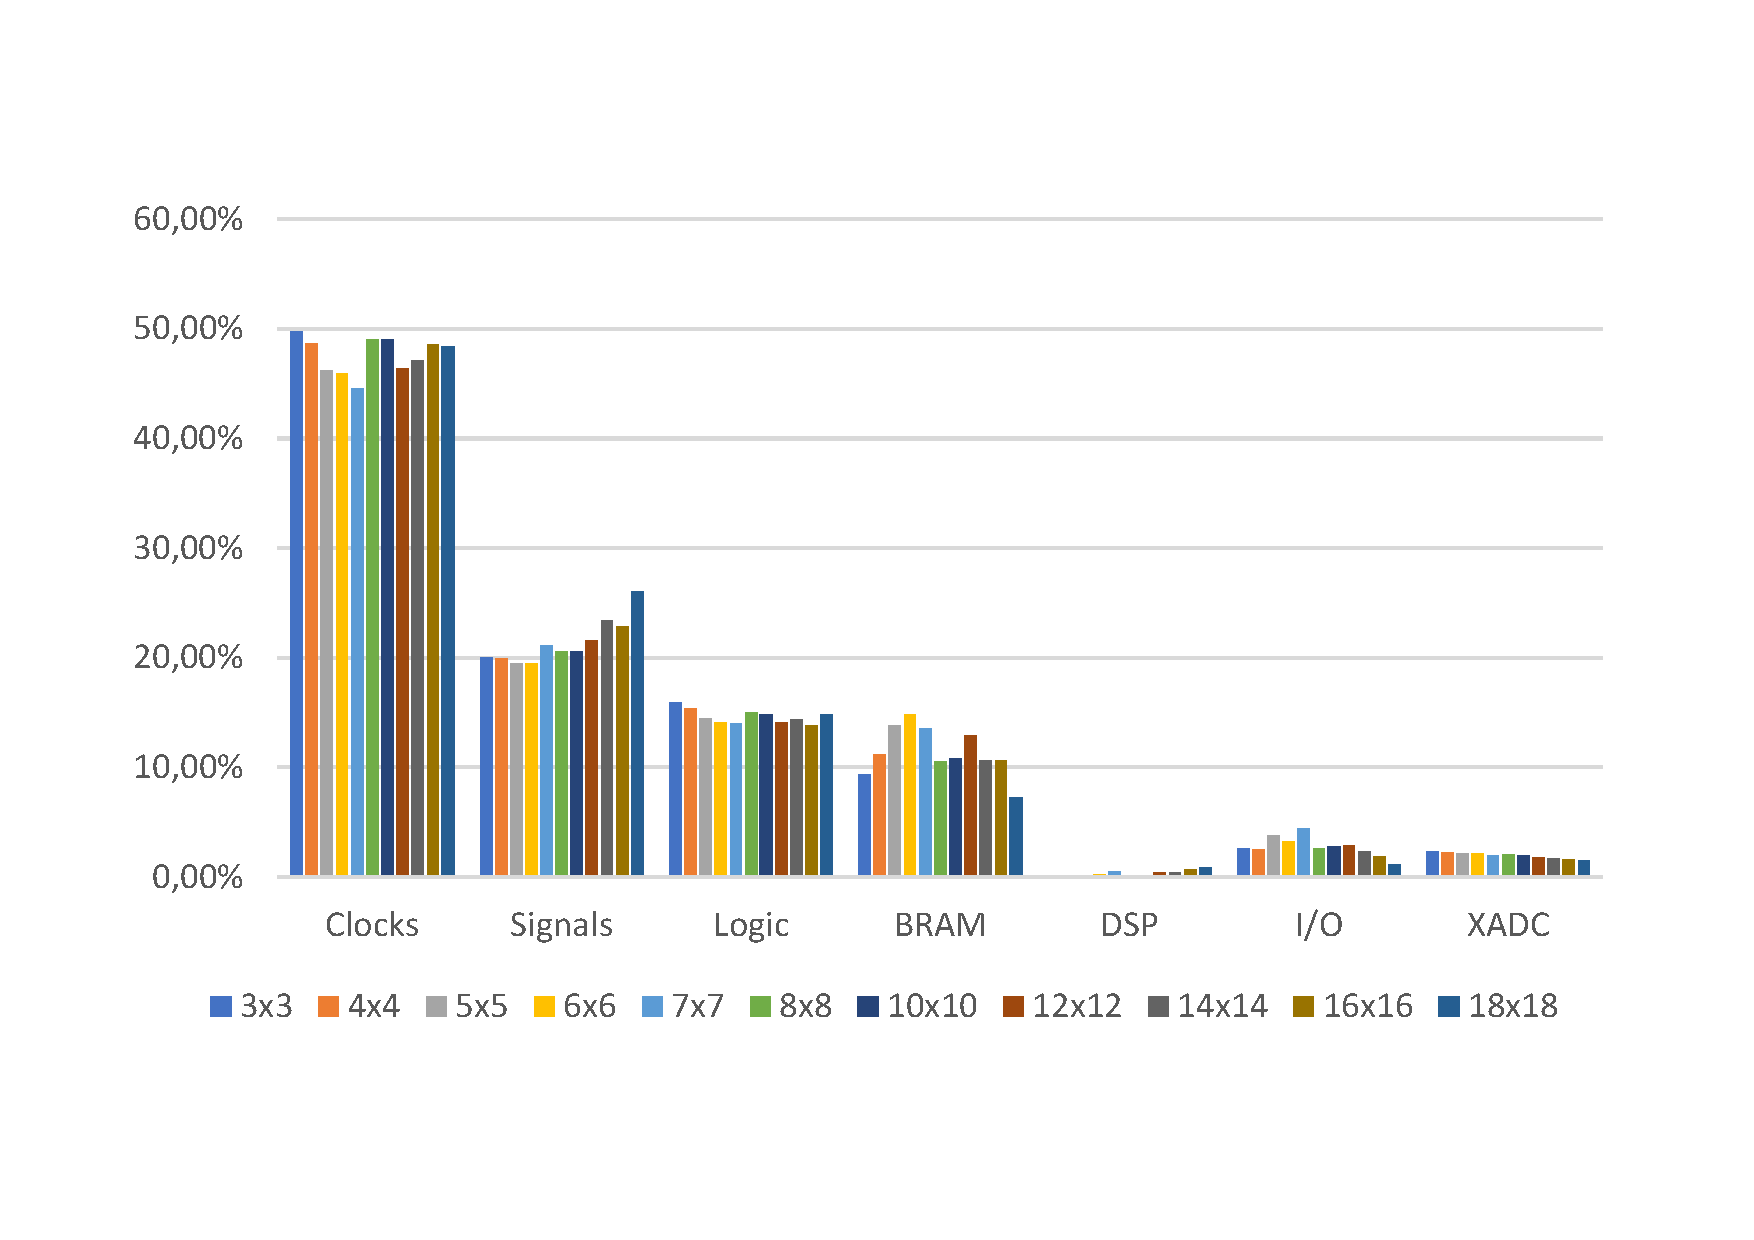
\includegraphics[scale=0.6,angle=0]{./figure/graphs/power_pldyn_div_int16_freq_30mhz.pdf}
\caption{Post Implementation Dynamic Power Consumption per entities in Programmable Logic with a clock frequency of 30 MHz and integer 16 PEs}
\label{fig:dynpowint16ent30}
\end{figure}
\begin{figure}[!htbp]
\centering
\captionsetup{justification=centering}
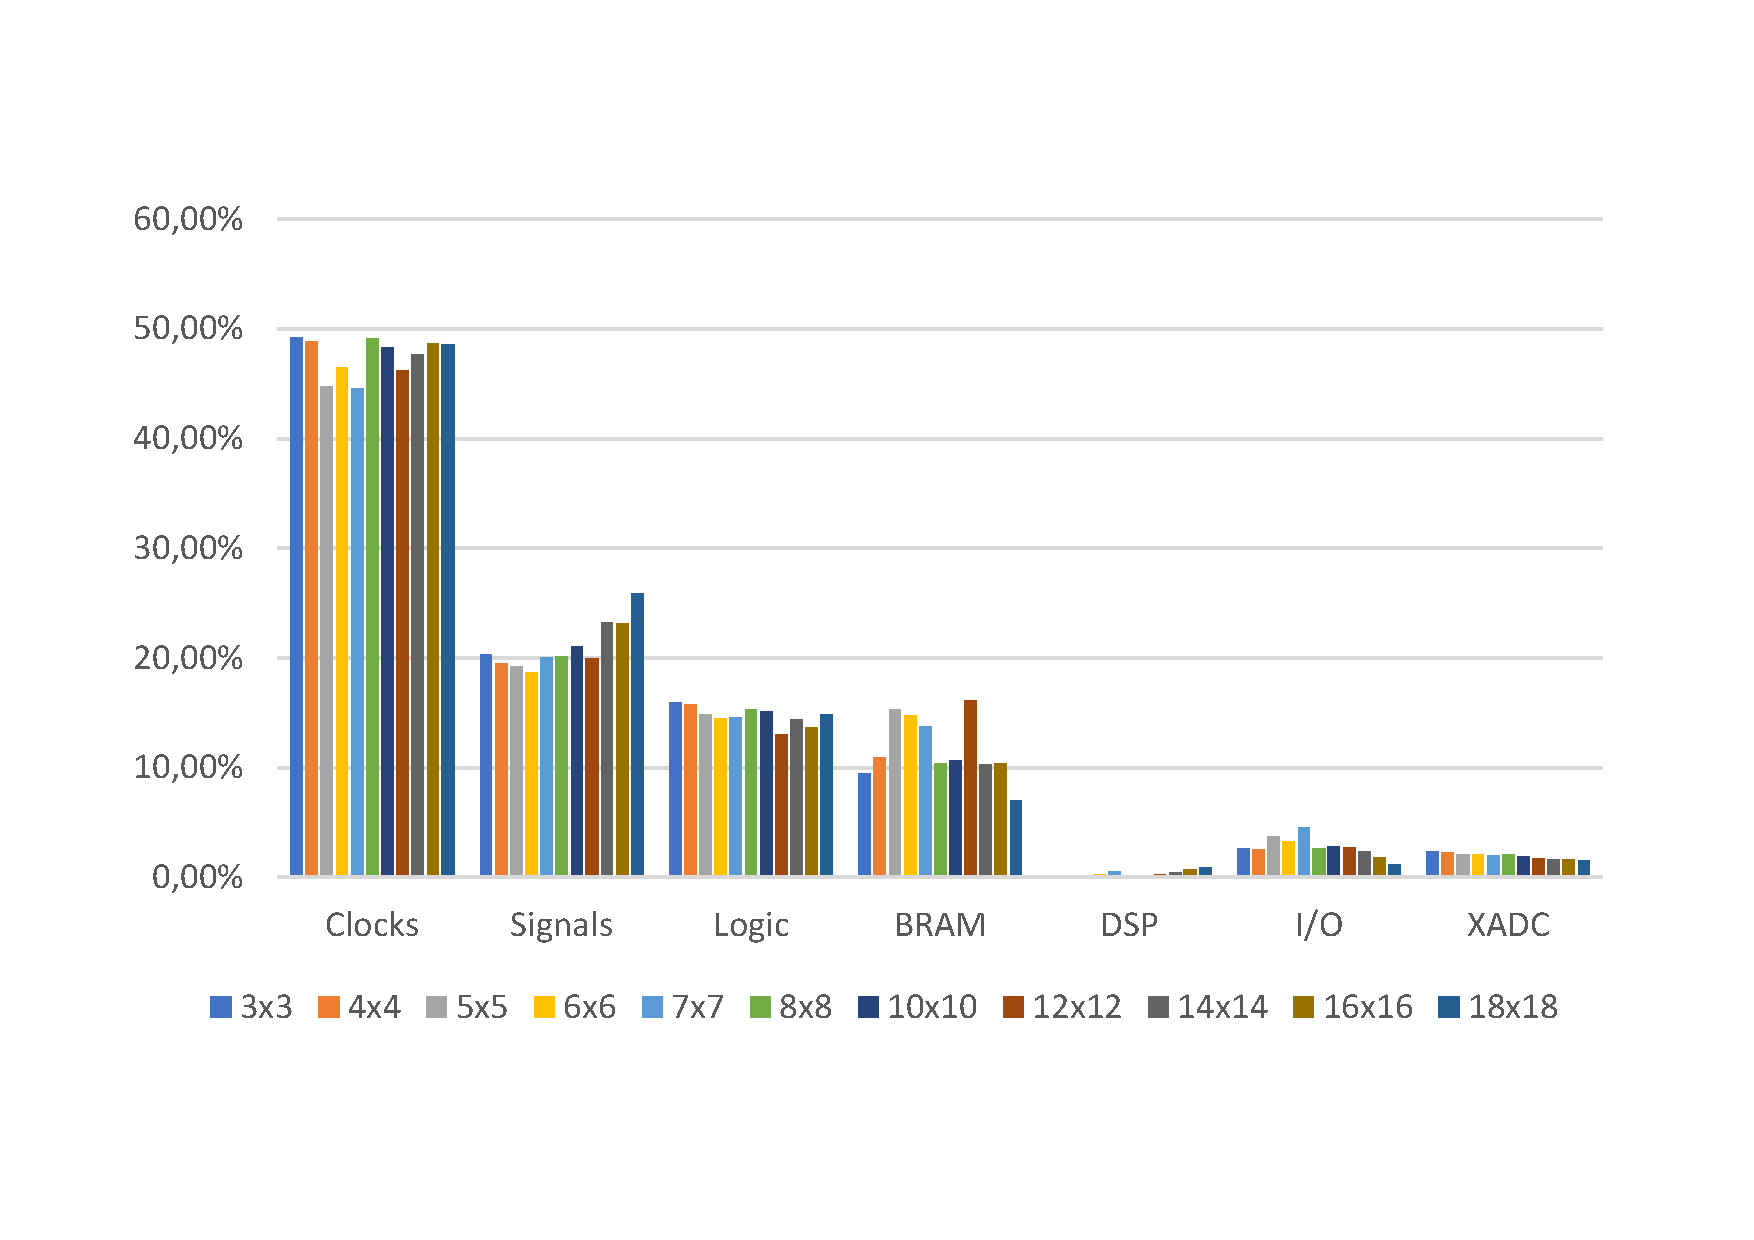
\includegraphics[scale=0.6,angle=0]{./figure/graphs/power_pldyn_div_int16_freq_50mhz.pdf}
\caption{Post Implementation Dynamic Power Consumption per entities in Programmable Logic with a clock frequency of 50 MHz and integer 16 PEs}
\label{fig:dynpowint16ent50}
\end{figure}
\begin{figure}[!htbp]
\centering
\captionsetup{justification=centering}
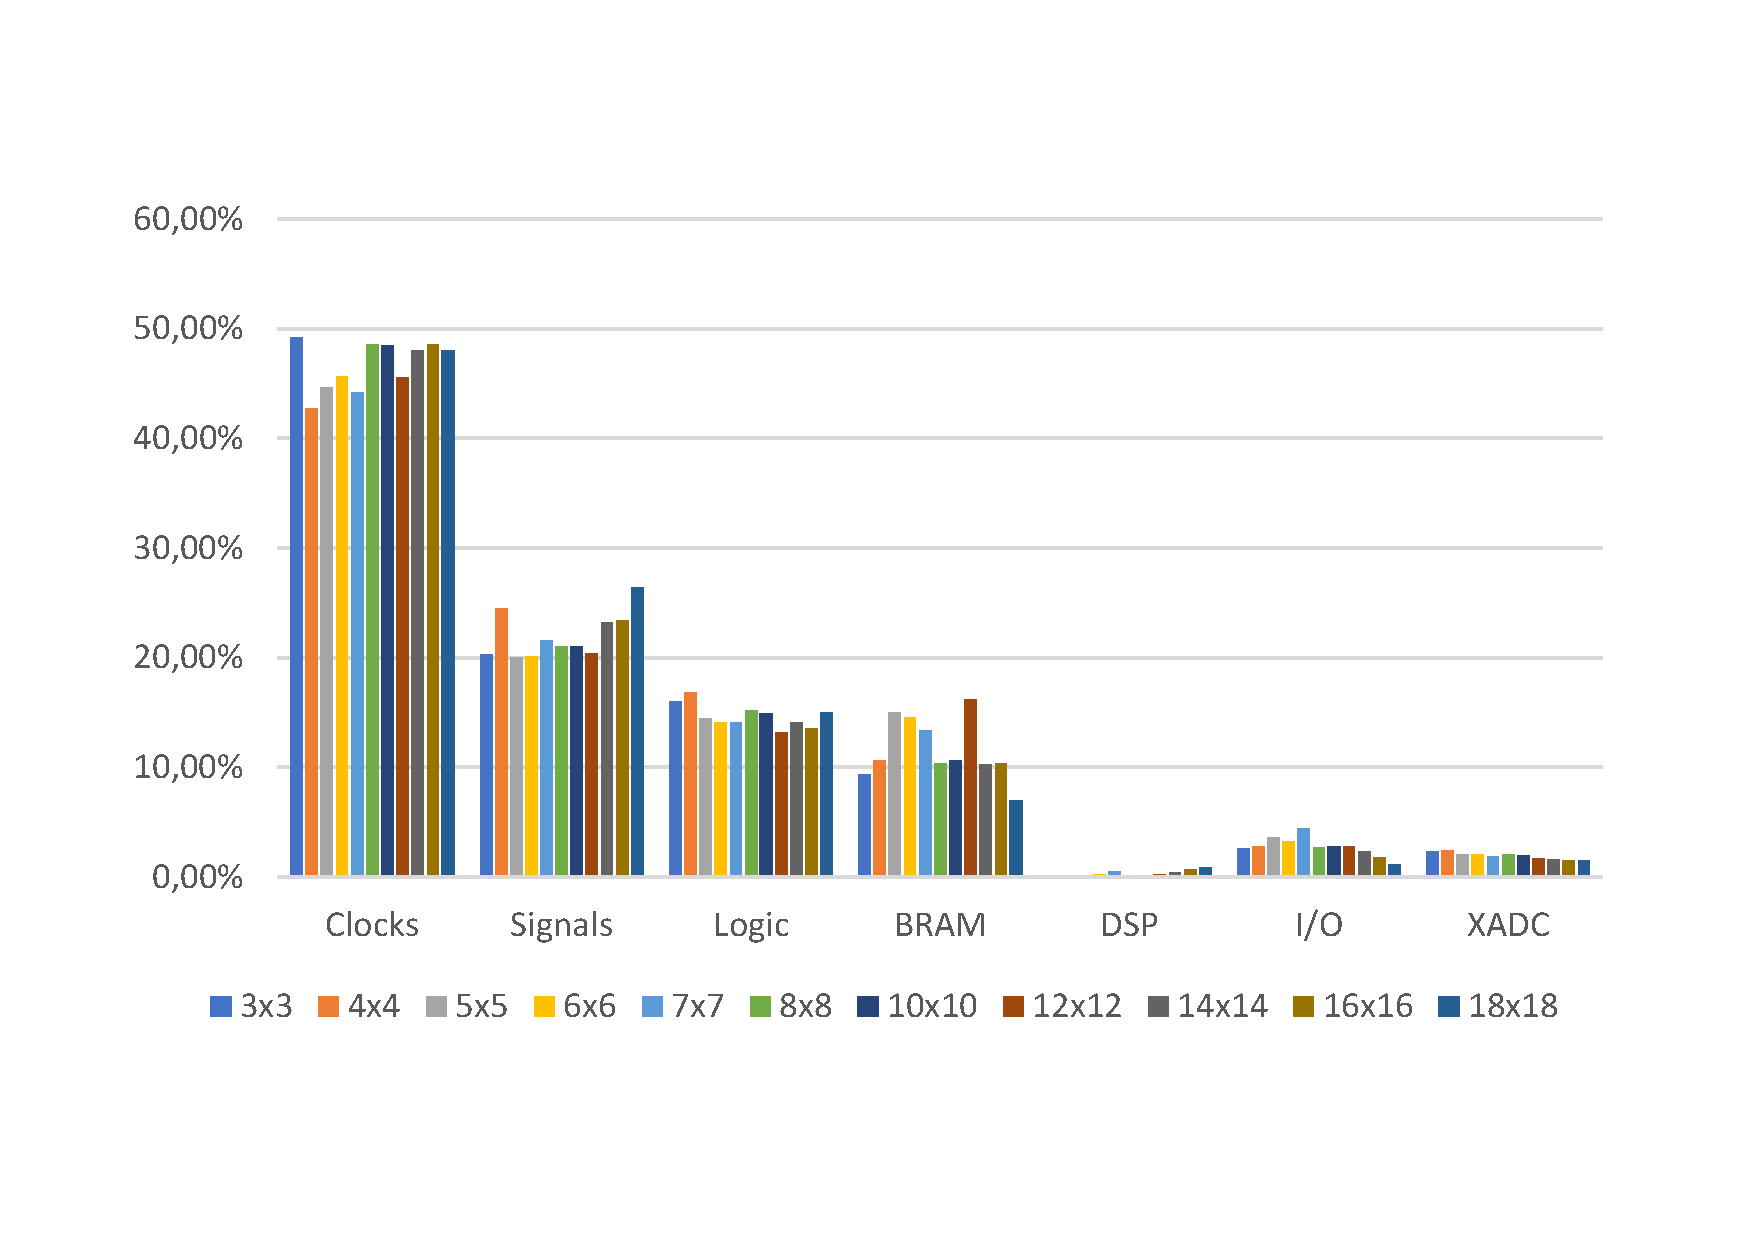
\includegraphics[scale=0.6,angle=0]{./figure/graphs/power_pldyn_div_int16_freq_80mhz.pdf}
\caption{Post Implementation Dynamic Power Consumption per entities in Programmable Logic with a clock frequency of 80 MHz and integer 16 PEs}
\label{fig:dynpowint16ent80}
\end{figure}
\begin{figure}[!htbp]
\centering
\captionsetup{justification=centering}
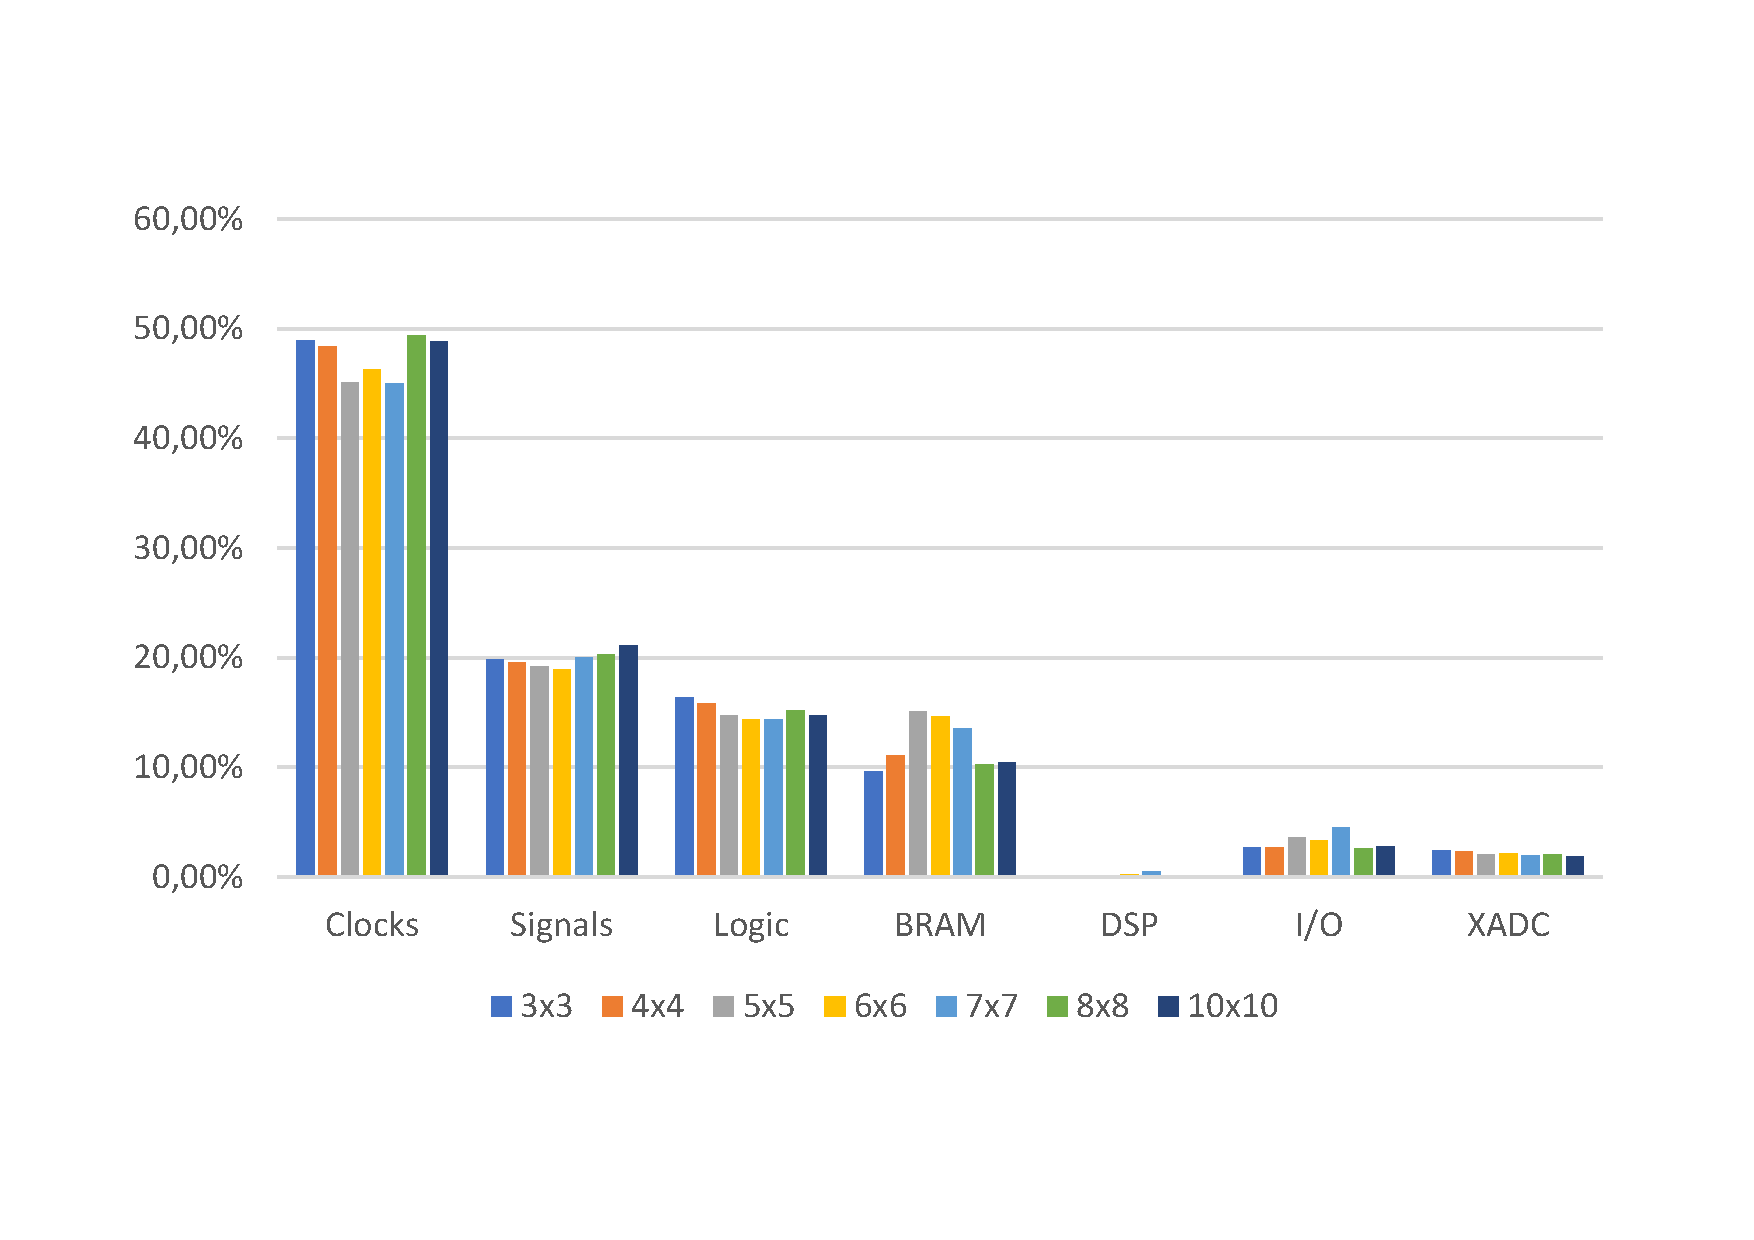
\includegraphics[scale=0.6,angle=0]{./figure/graphs/power_pldyn_div_int16_freq_100mhz.pdf}
\caption{Post Implementation Dynamic Power Consumption per entities in Programmable Logic with a clock frequency of 100 MHz and integer 16 PEs}
\label{fig:dynpowint16ent100}
\end{figure}
\newpage
\item Integer 32:\\
From now on, the MXU sizes and the frequencies will show a reduction in their values, this is manly because big designs (with almost full FPGA's utilization) are not able to meet anymore the timing requirements.
\begin{figure}[!htbp]
\centering
\captionsetup{justification=centering}
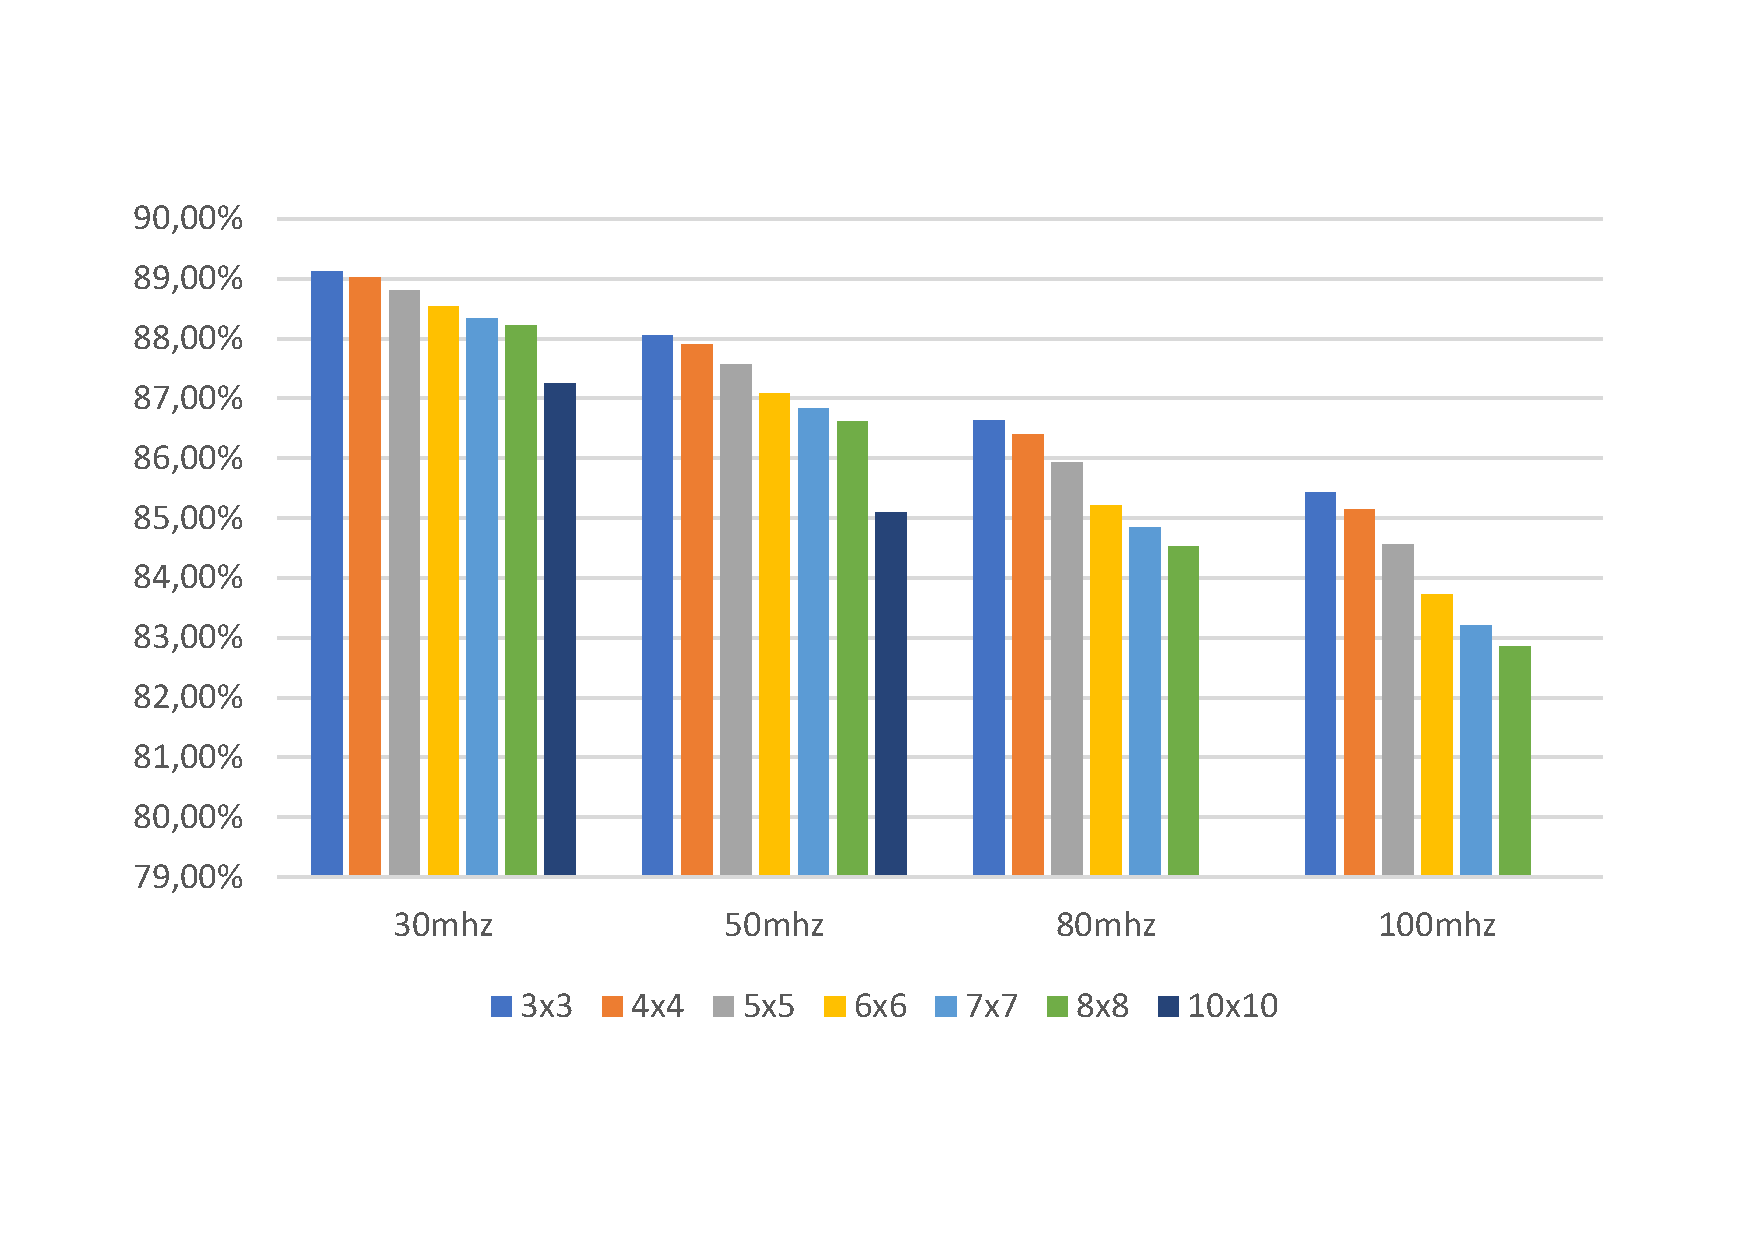
\includegraphics[scale=0.5,angle=0]{./figure/graphs/power_ps_int32_freq.pdf}
\caption{Post Implementation Power Consumption of Processing System for integer 32 PEs}
\label{fig:powint32}
\end{figure}
\begin{figure}[!htbp]
\centering
\captionsetup{justification=centering}
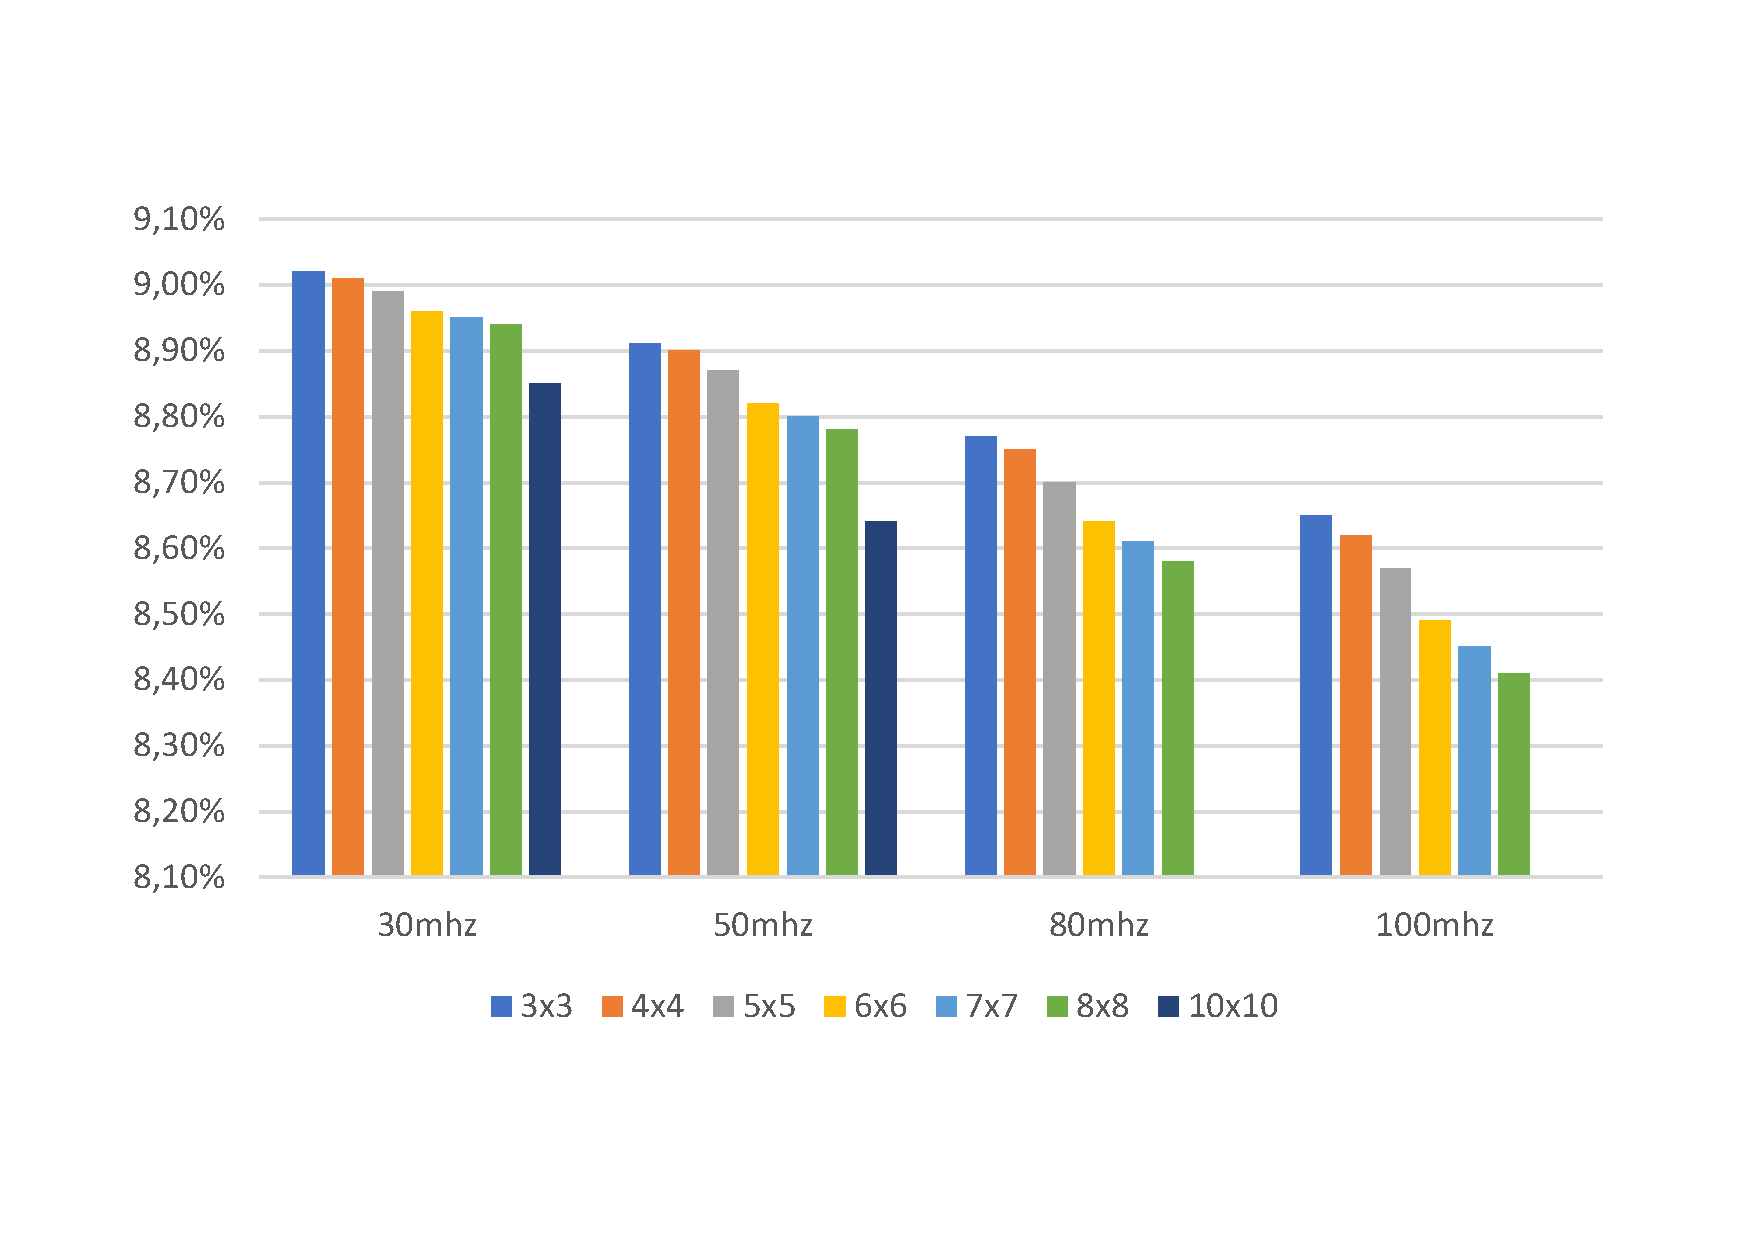
\includegraphics[scale=0.5,angle=0]{./figure/graphs/power_plstatic_int32_freq.pdf}
\caption{Post Implementation Static Power Consumption Programmable logic for integer 32 PEs }
\label{fig:staticpowint32}
\end{figure}
\begin{figure}[!htbp]
\centering
\captionsetup{justification=centering}
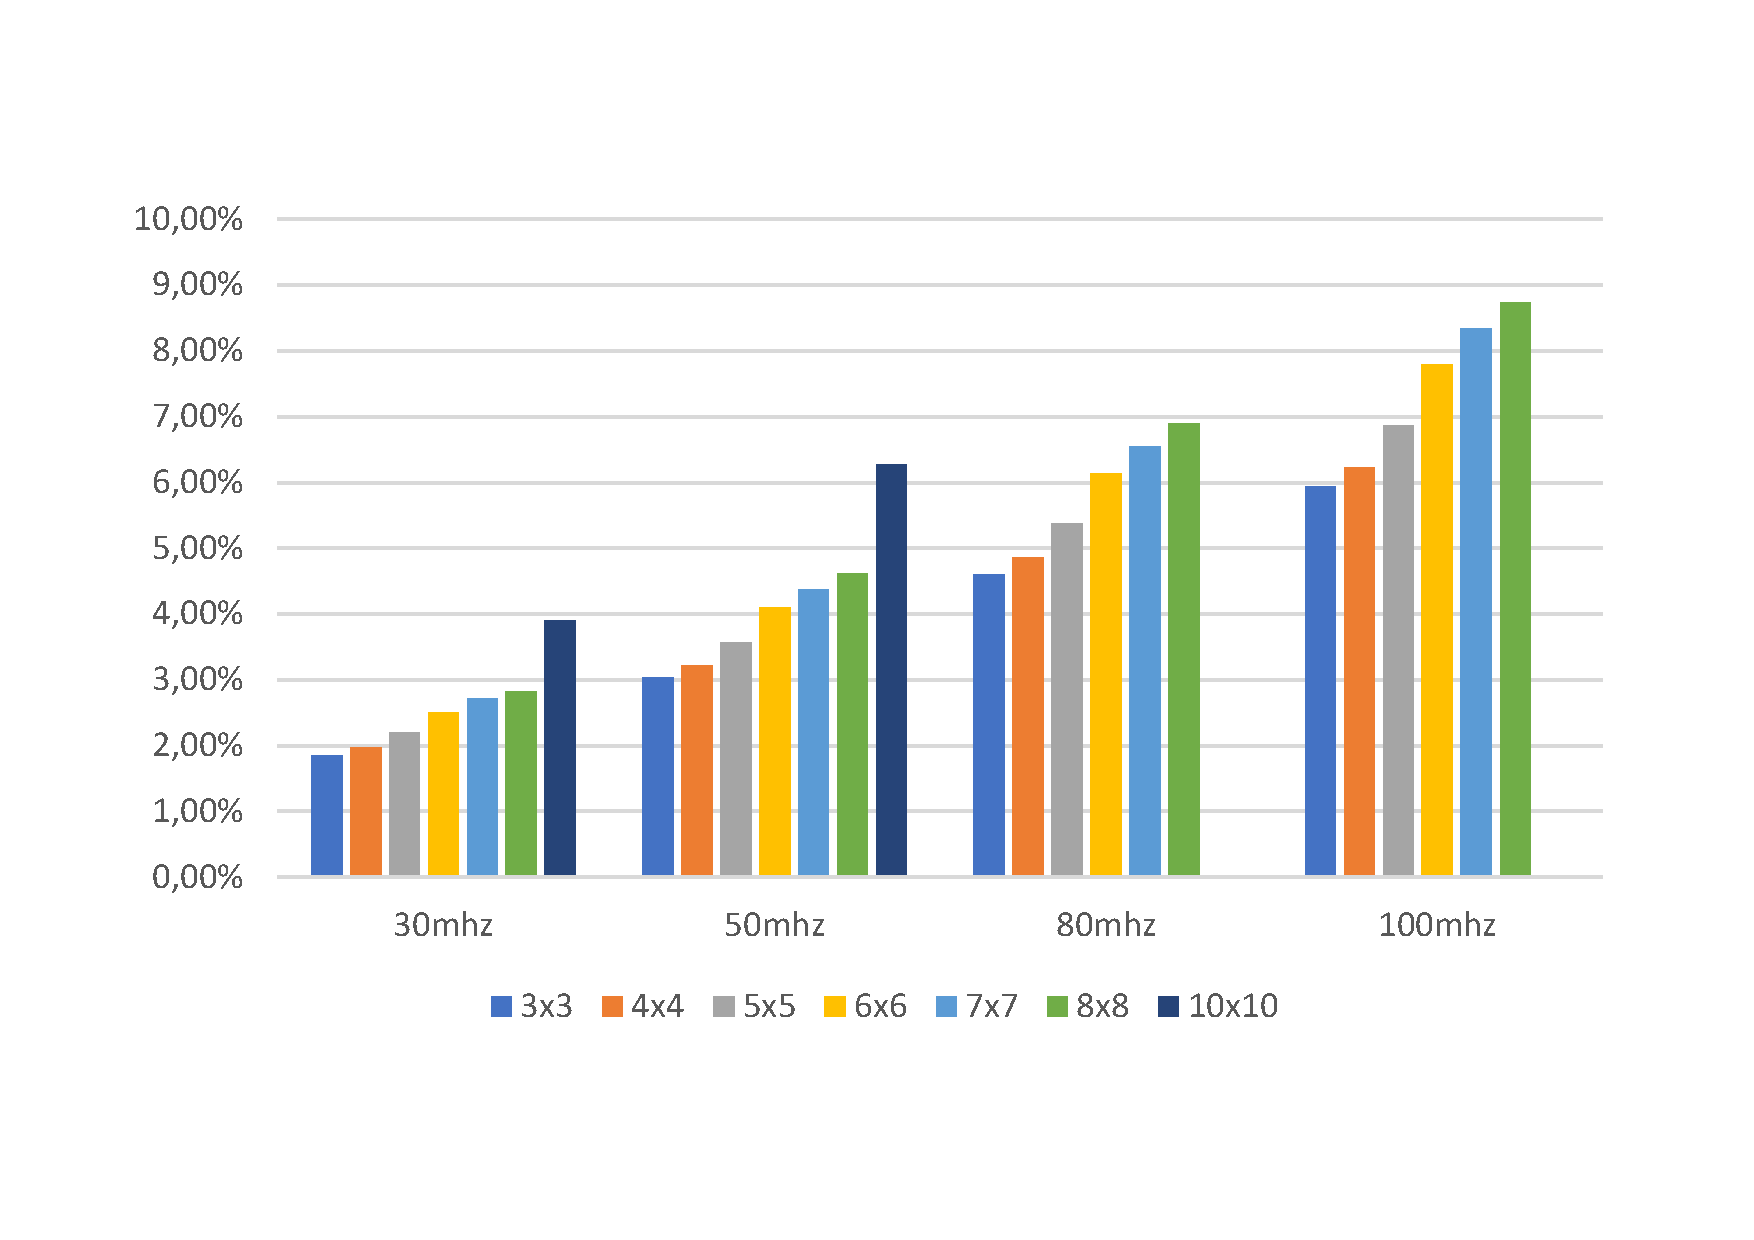
\includegraphics[scale=0.5,angle=0]{./figure/graphs/power_pldyn_int32_freq.pdf}
\caption{Post Implementation Dynamic Power Consumption per Programmable logic with integer 32 PEs}
\label{fig:dynpowint32}
\end{figure}
\begin{figure}[!htbp]
\centering
\captionsetup{justification=centering}
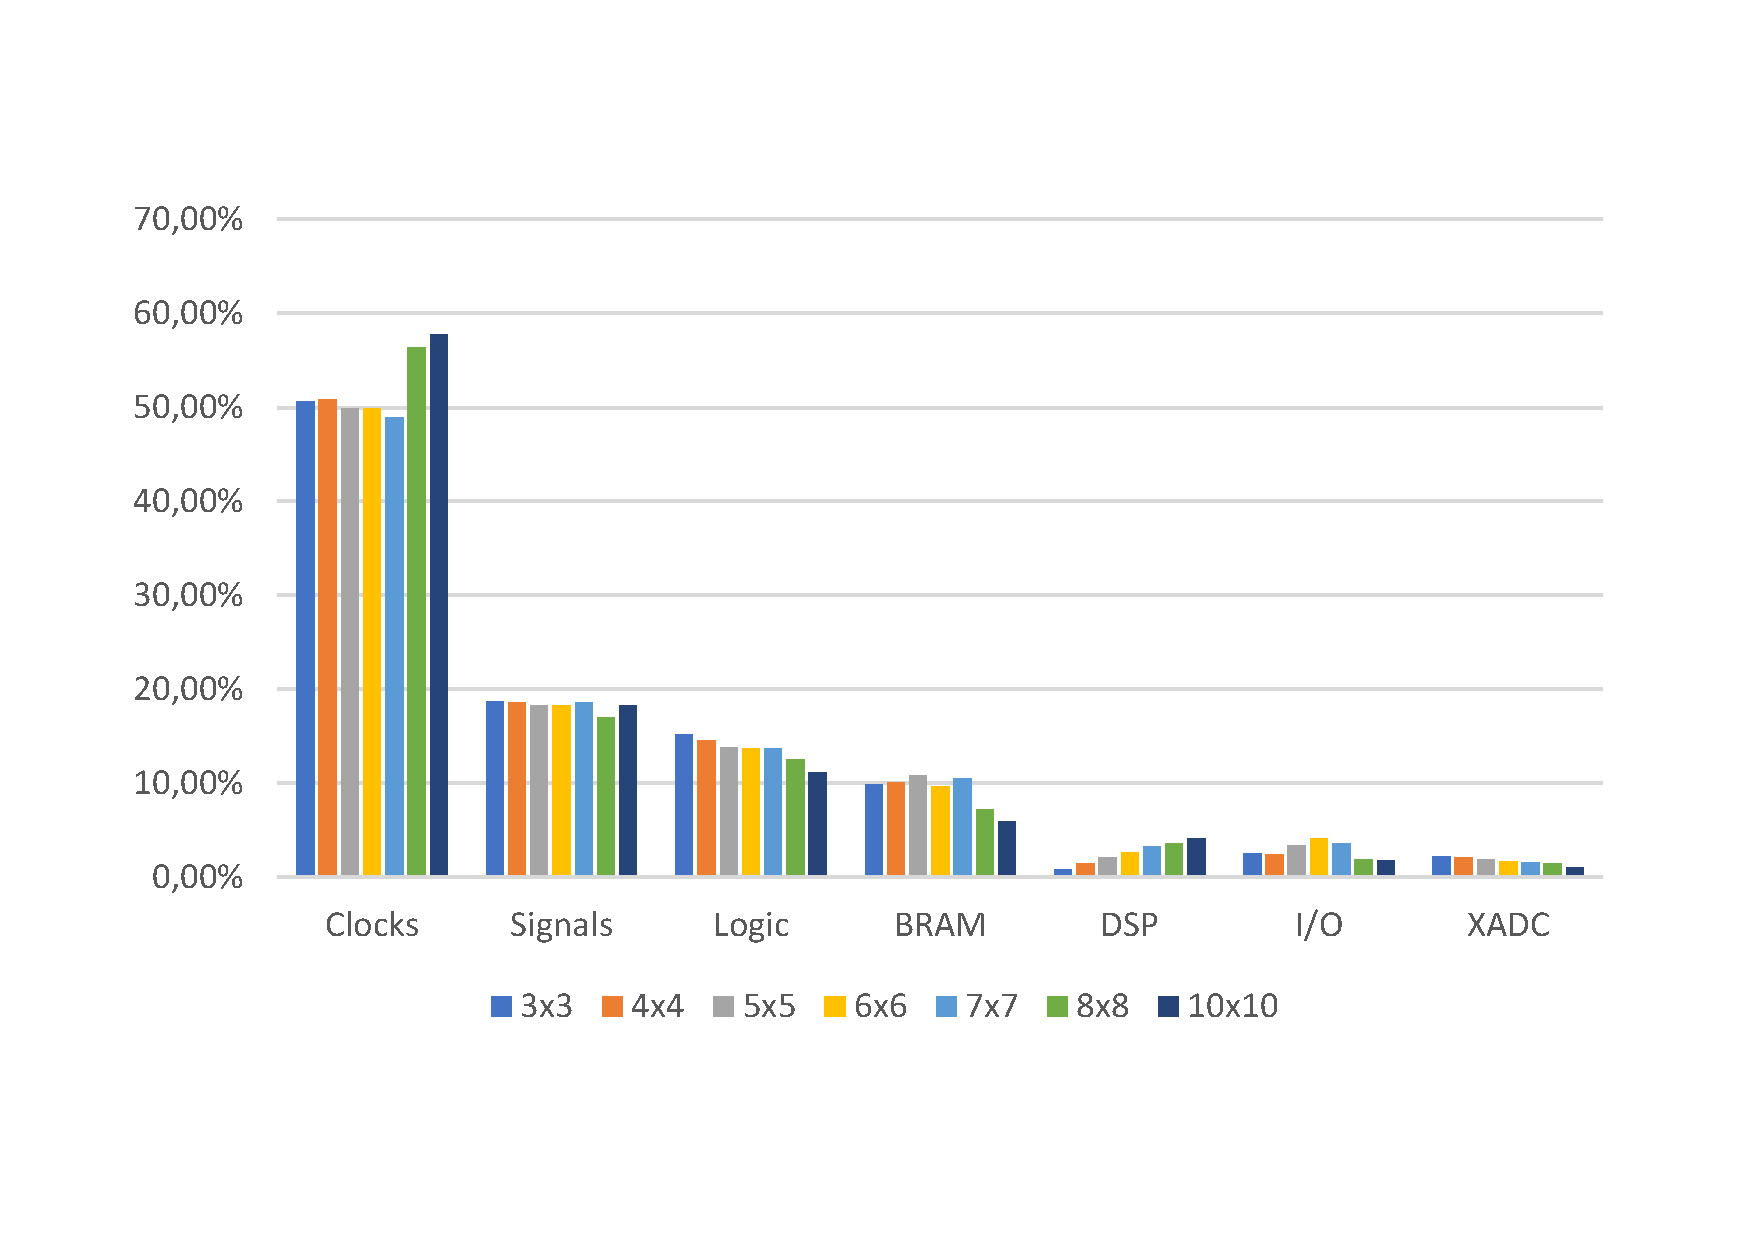
\includegraphics[scale=0.6,angle=0]{./figure/graphs/power_pldyn_div_int32_freq_30mhz.pdf}
\caption{Post Implementation Dynamic Power Consumption per entities in Programmable Logic with a clock frequency of 30 MHz and integer 32 PEs}
\label{fig:dynpowint32ent30}
\end{figure}
\begin{figure}[!htbp]
\centering
\captionsetup{justification=centering}
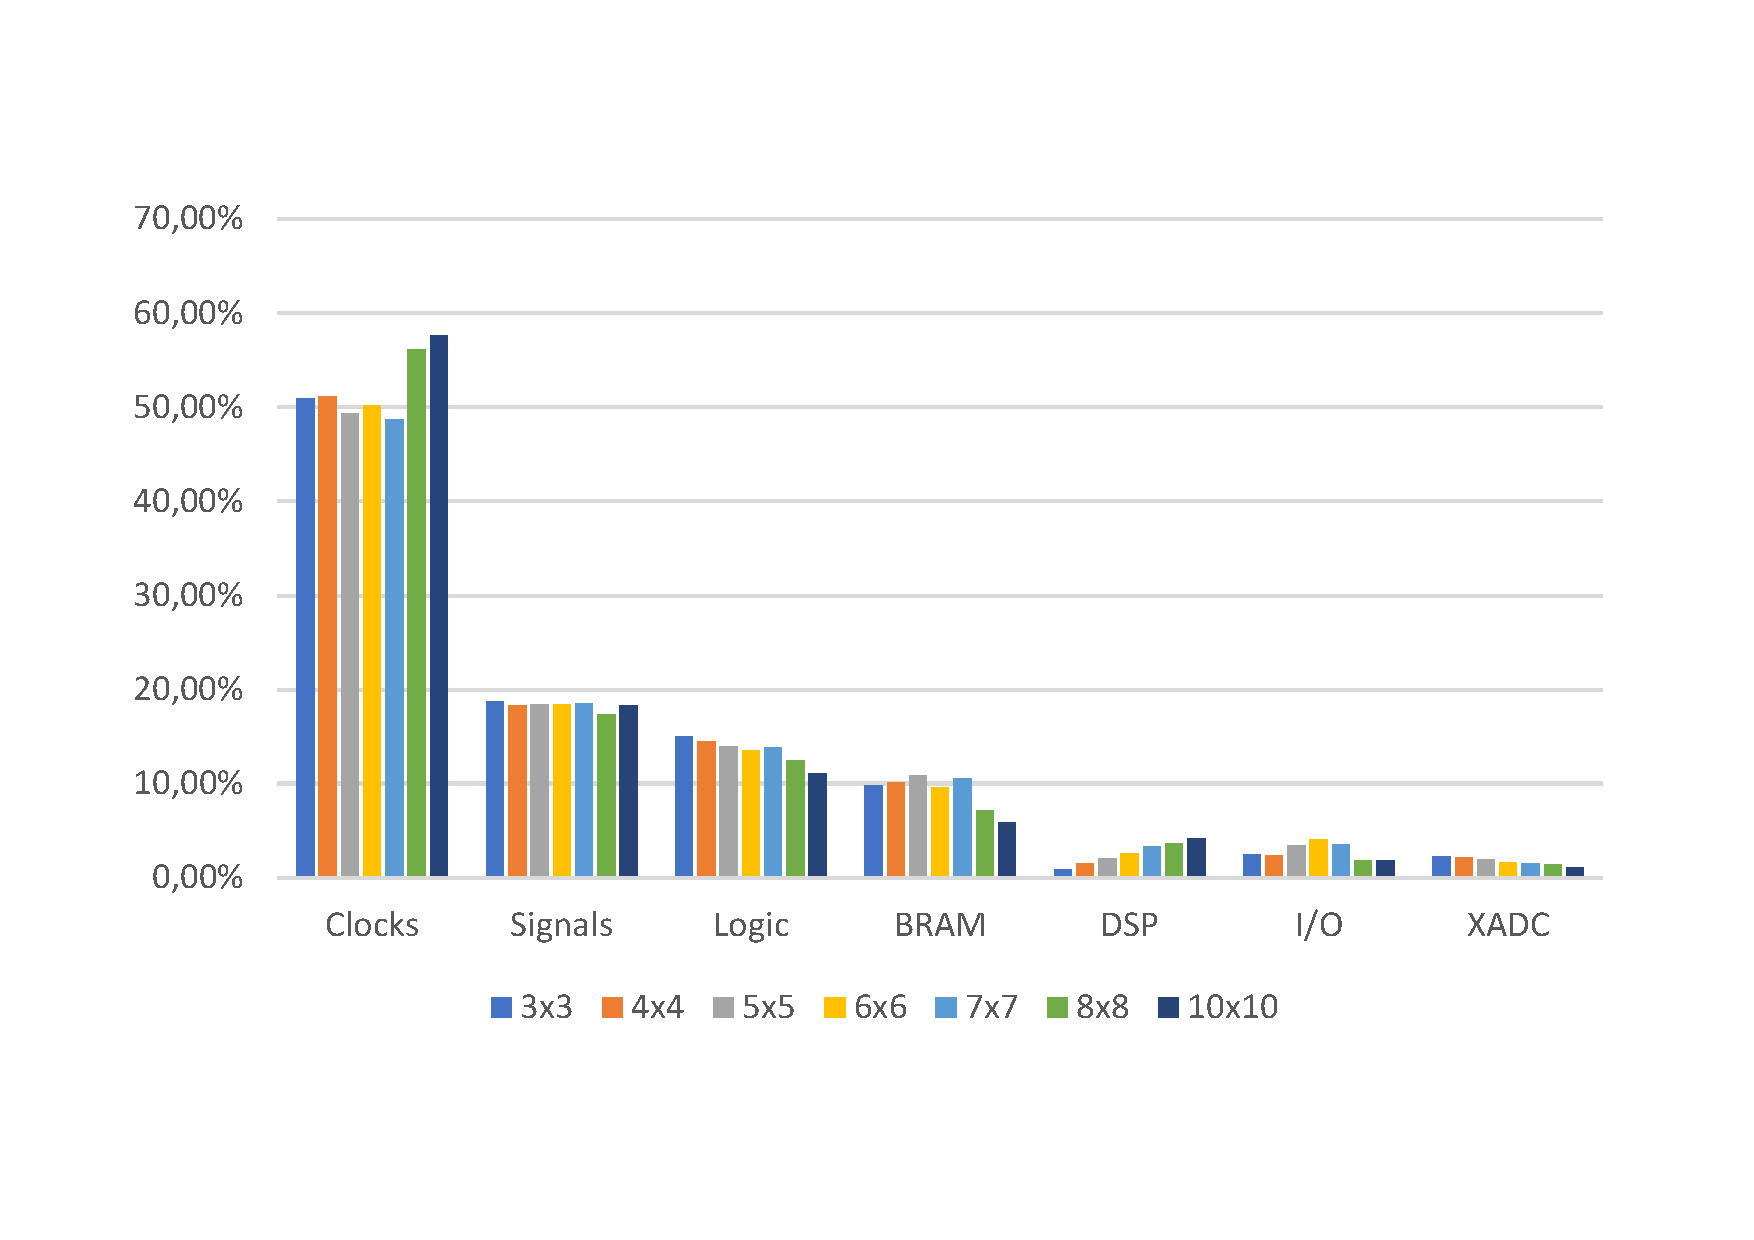
\includegraphics[scale=0.6,angle=0]{./figure/graphs/power_pldyn_div_int32_freq_50mhz.pdf}
\caption{Post Implementation Dynamic Power Consumption per entities in Programmable Logic with a clock frequency of 50 MHz and integer 32 PEs}
\label{fig:dynpowint32ent50}
\end{figure}
\begin{figure}[!htbp]
\centering
\captionsetup{justification=centering}
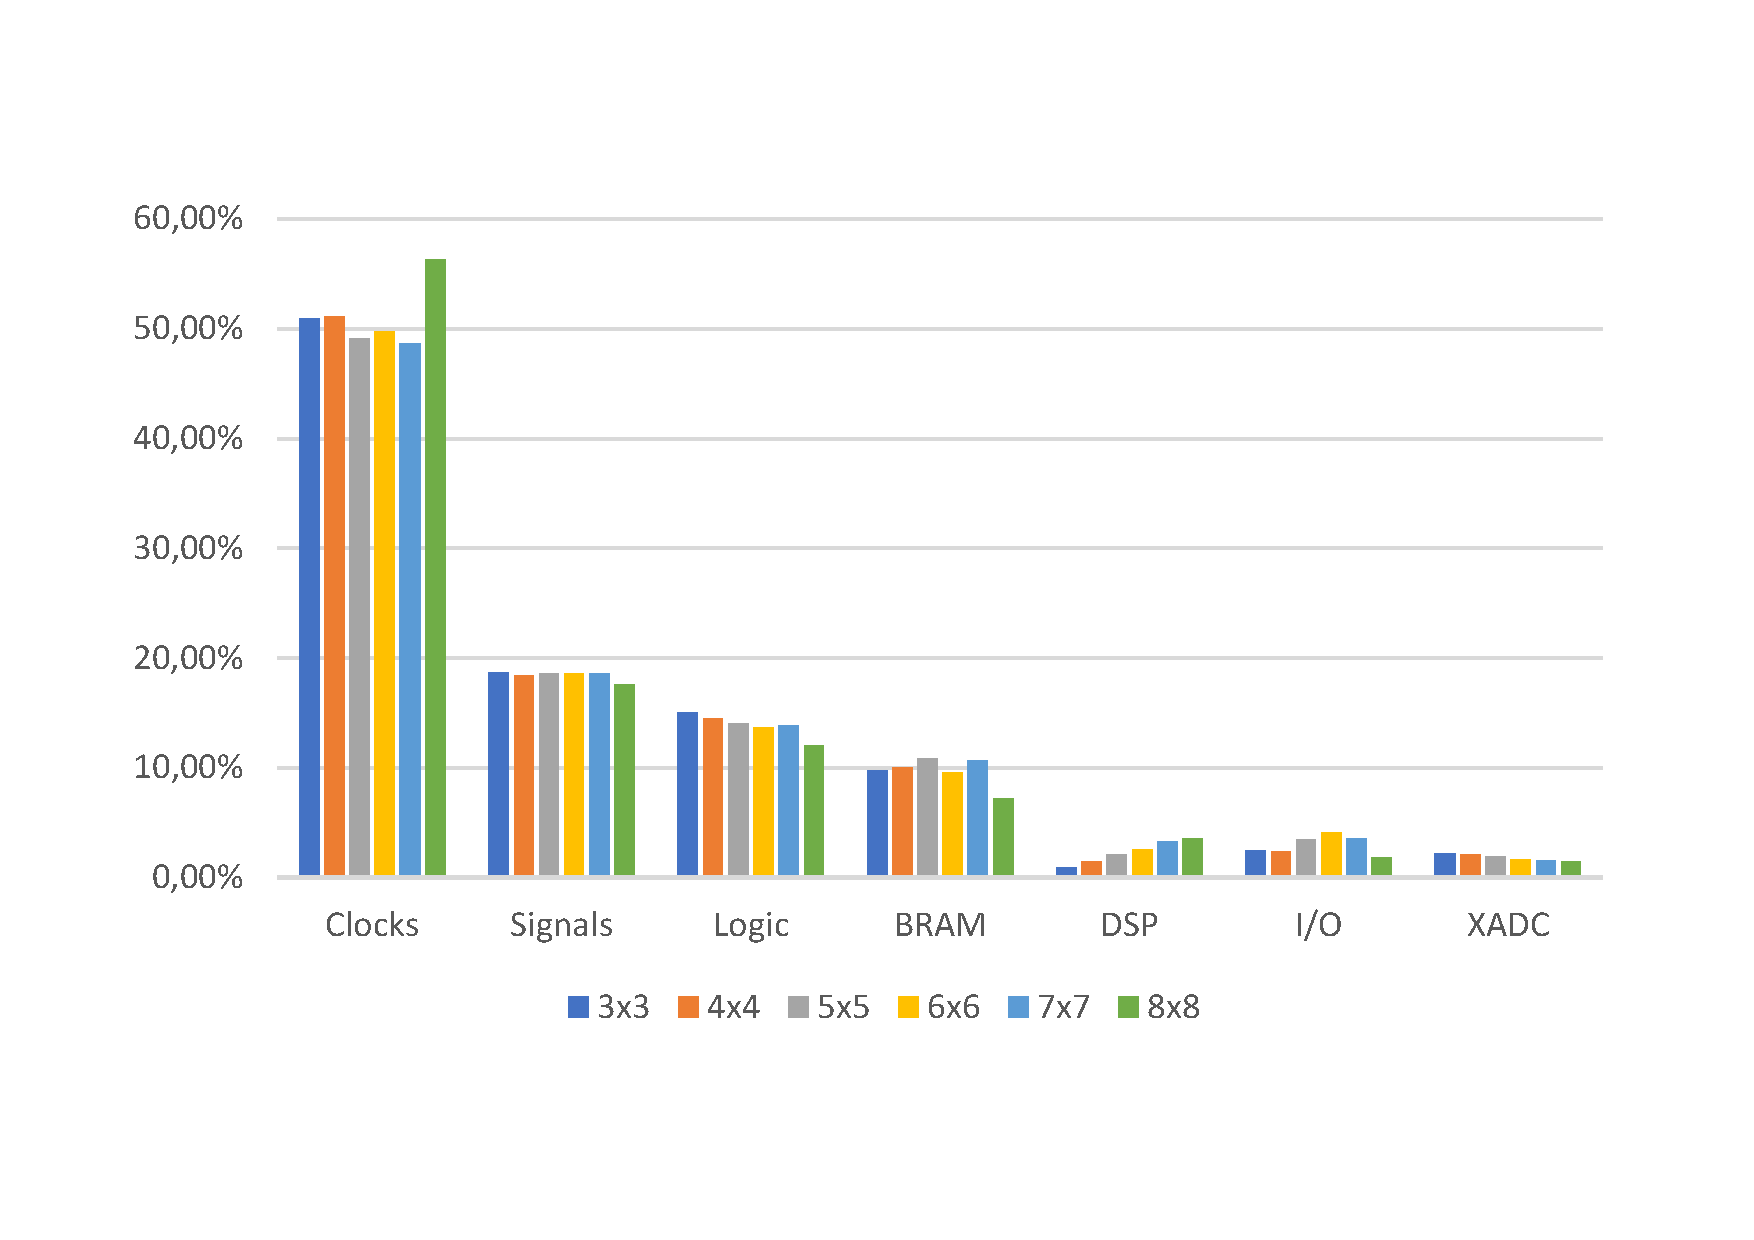
\includegraphics[scale=0.6,angle=0]{./figure/graphs/power_pldyn_div_int32_freq_80mhz.pdf}
\caption{Post Implementation Dynamic Power Consumption per entities in Programmable Logic with a clock frequency of 80 MHz and integer 32 PEs}
\label{fig:dynpowint32ent80}
\end{figure}
\begin{figure}[!htbp]
\centering
\captionsetup{justification=centering}
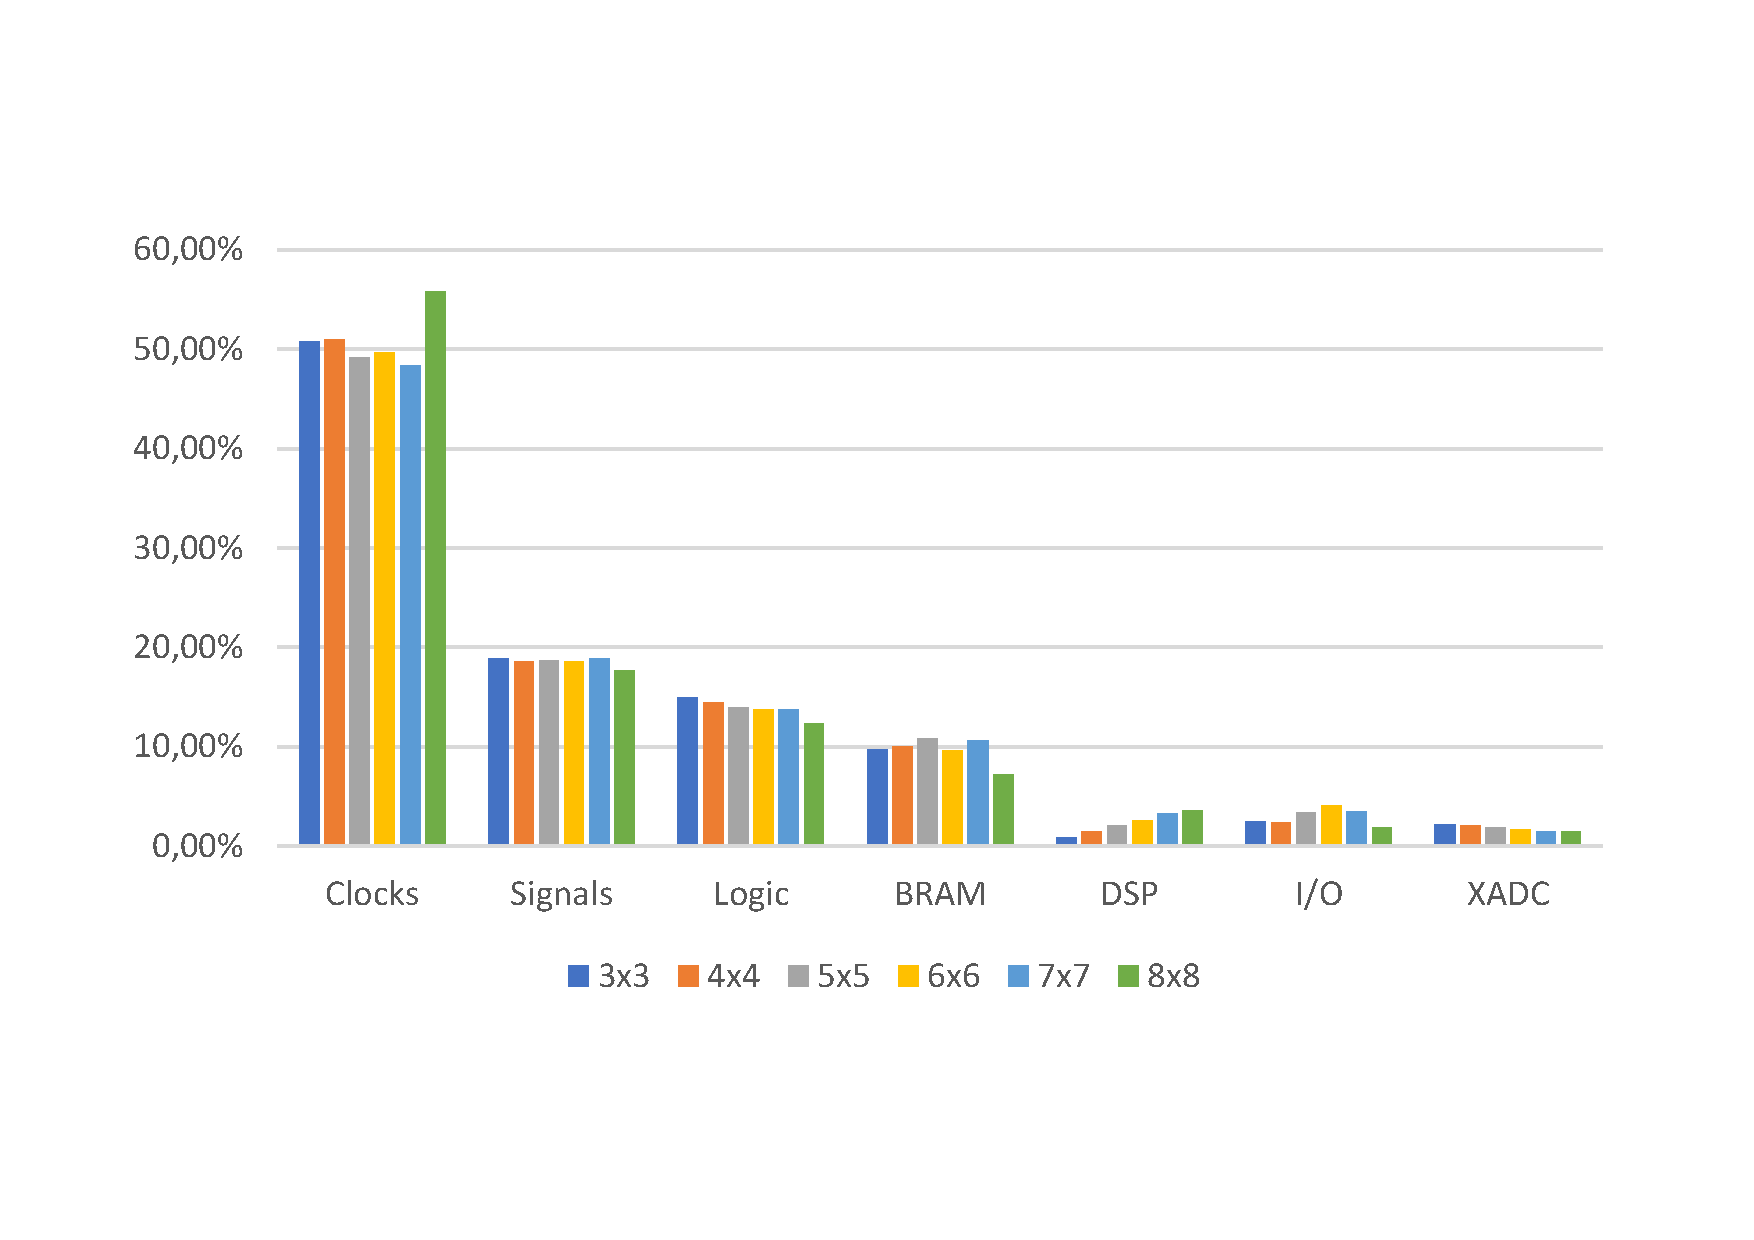
\includegraphics[scale=0.6,angle=0]{./figure/graphs/power_pldyn_div_int32_freq_100mhz.pdf}
\caption{Post Implementation Dynamic Power Consumption per entities in Programmable Logic with a clock frequency of 100 MHz and integer 32 PEs}
\label{fig:dynpowint32ent100}
\end{figure}

It is worth to mention the power consumed by the DSP entities, comparing to integer 8 and 16 PEs, is bigger. The main reason is that there is no more one to one mapping between PEs and DSP entities.

\item Integer 64:
\begin{figure}[!htbp]
\centering
\captionsetup{justification=centering}
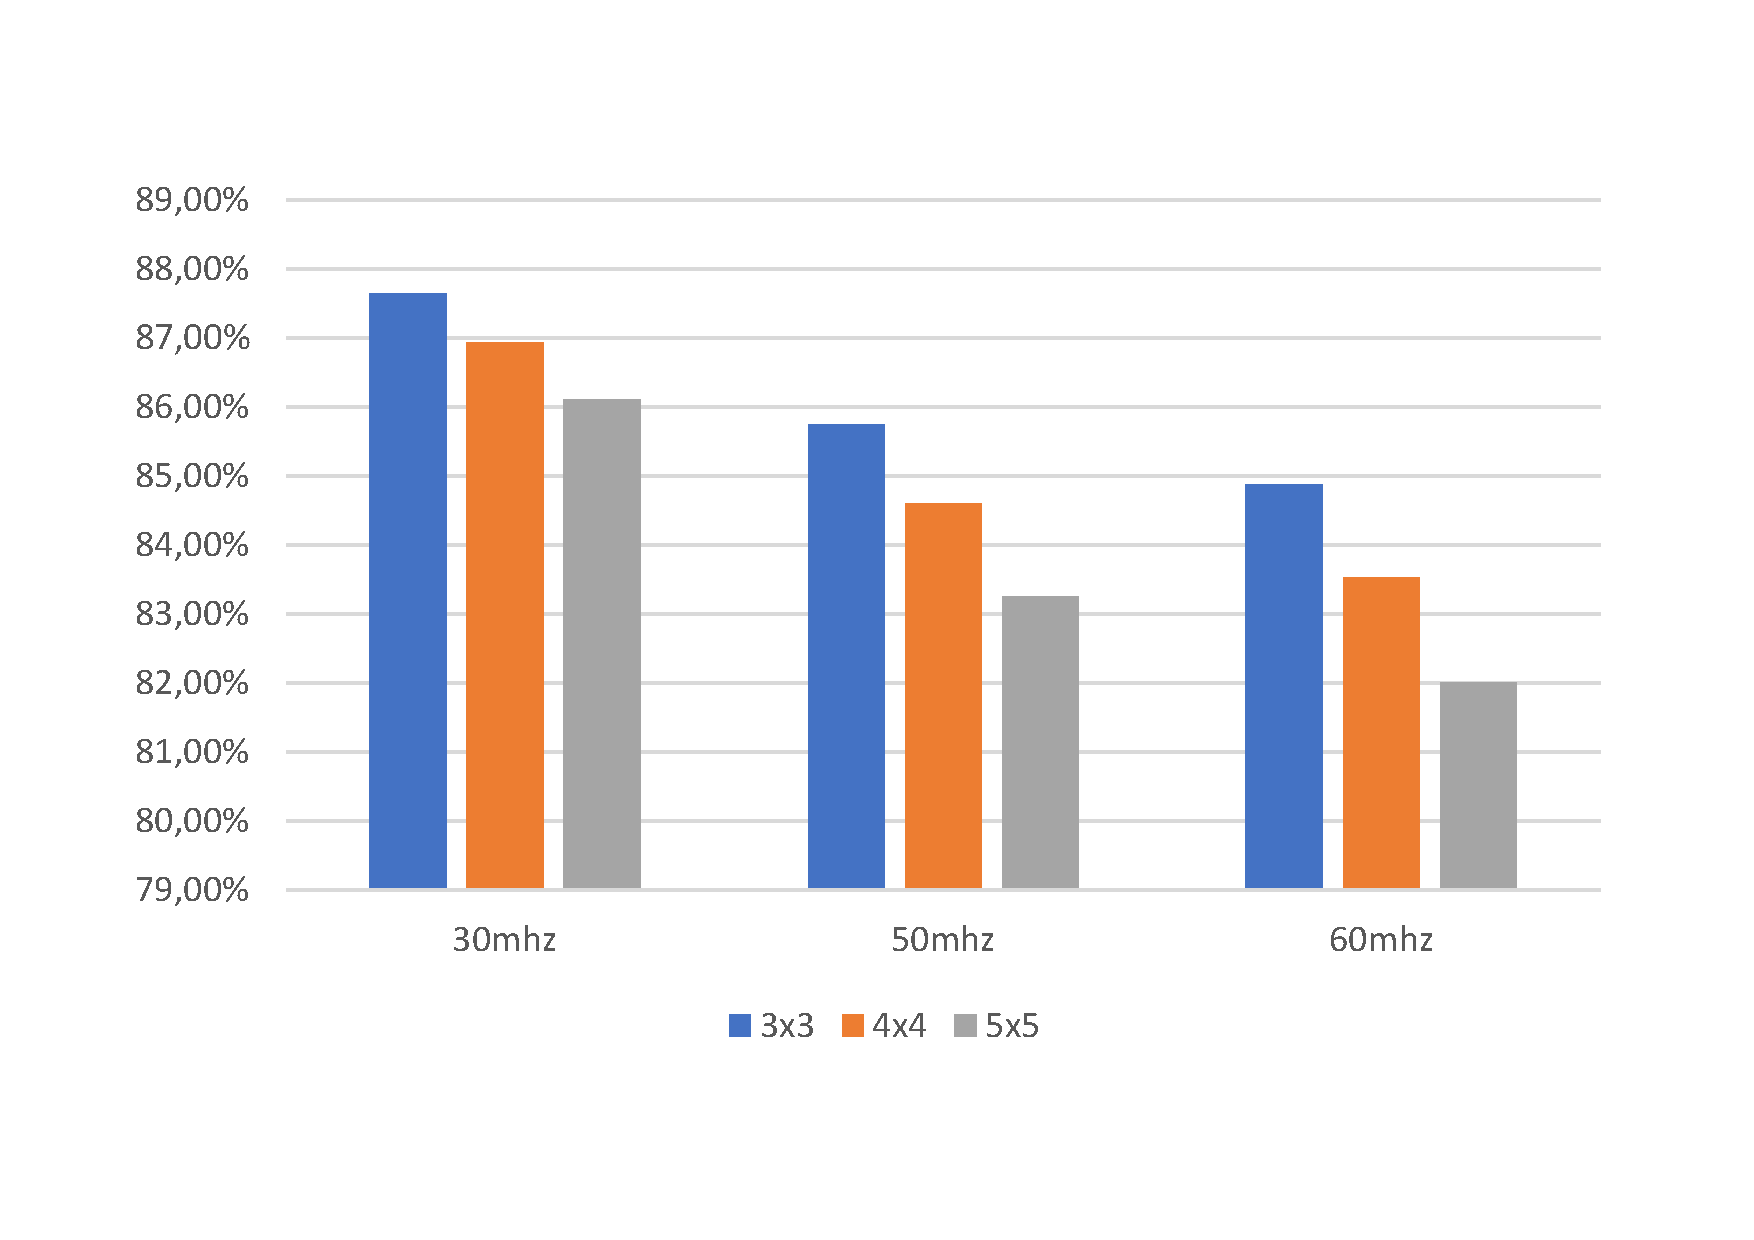
\includegraphics[scale=0.5,angle=0]{./figure/graphs/power_ps_int64_freq.pdf}
\caption{Post Implementation Power Consumption of Processing System for integer 64 PEs}
\label{fig:powint64}
\end{figure}
\begin{figure}[!htbp]
\centering
\captionsetup{justification=centering}
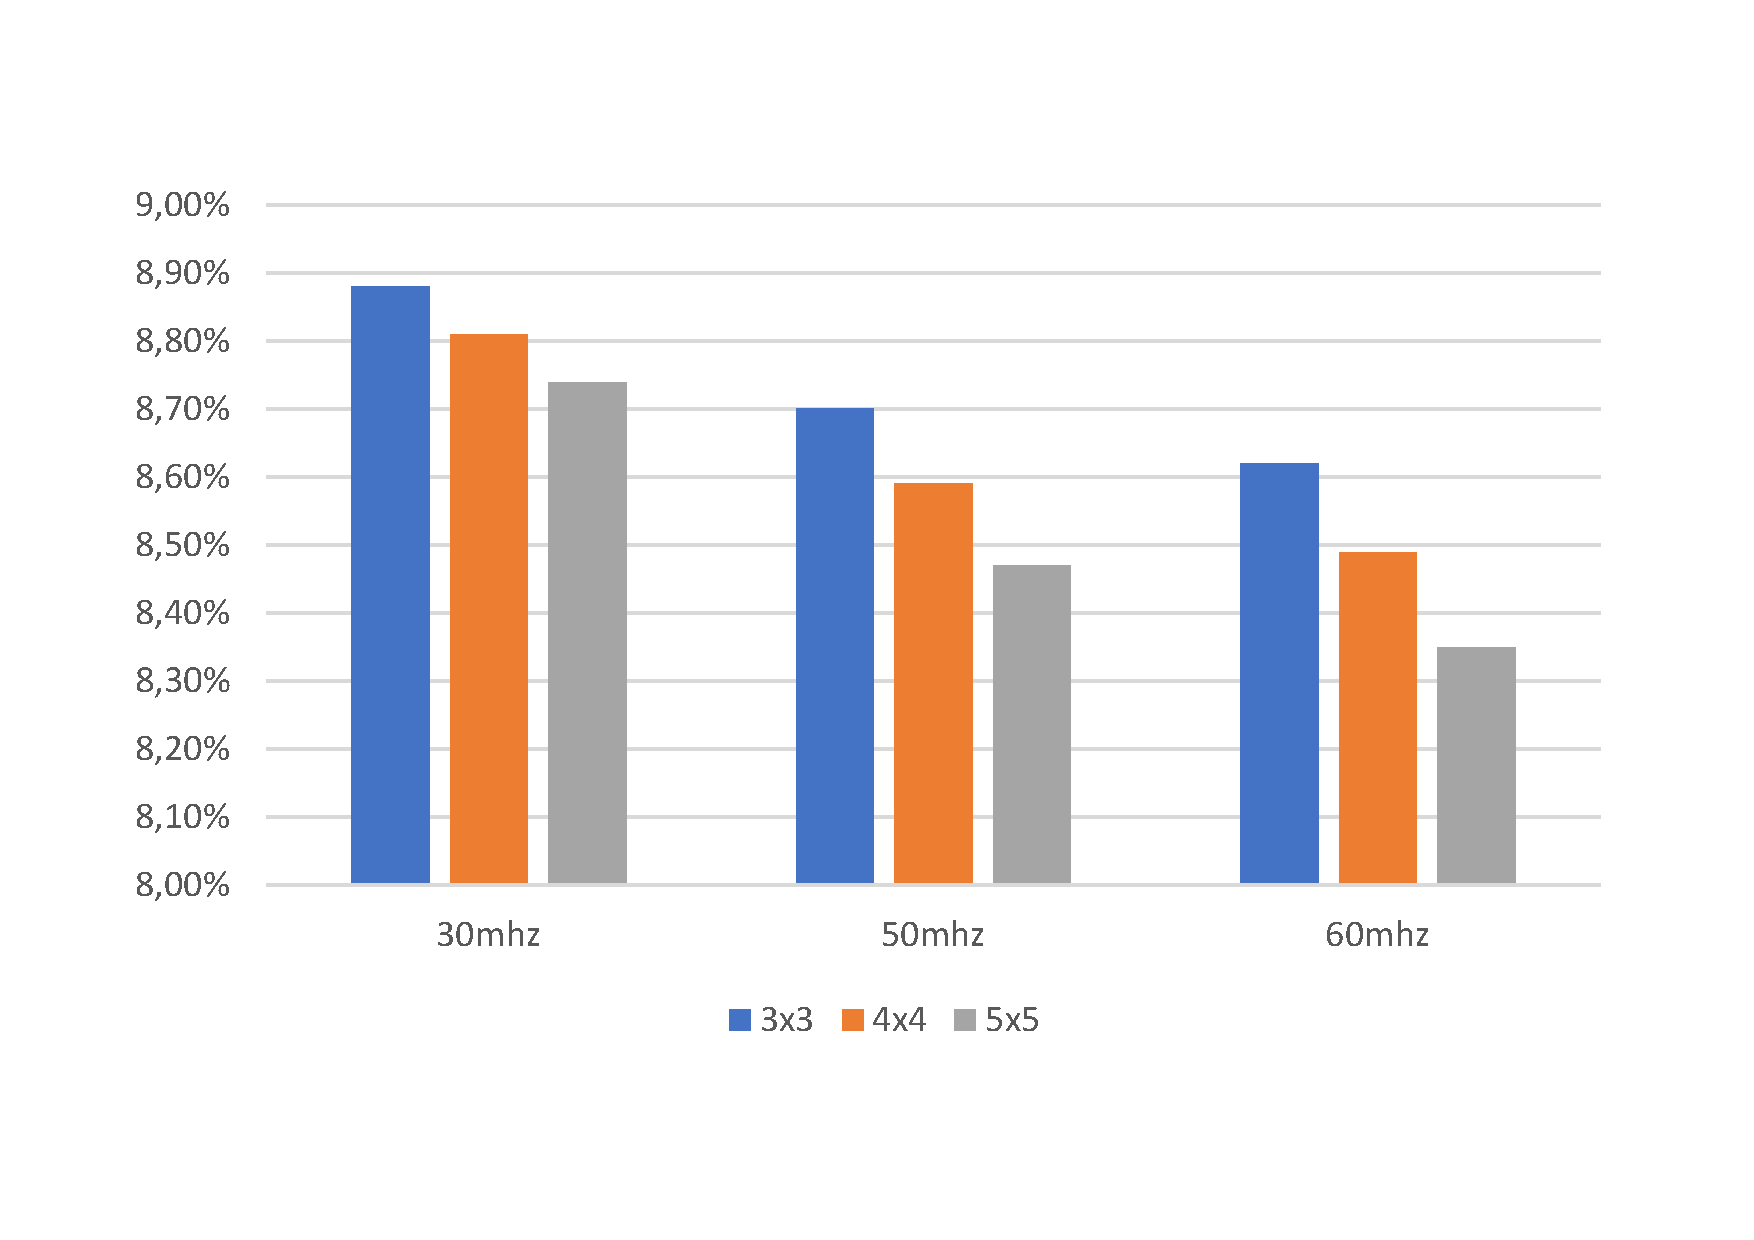
\includegraphics[scale=0.5,angle=0]{./figure/graphs/power_plstatic_int64_freq.pdf}
\caption{Post Implementation Static Power Consumption Programmable logic for integer 64 PEs }
\label{fig:staticpowint64}
\end{figure}
\begin{figure}[!htbp]
\centering
\captionsetup{justification=centering}
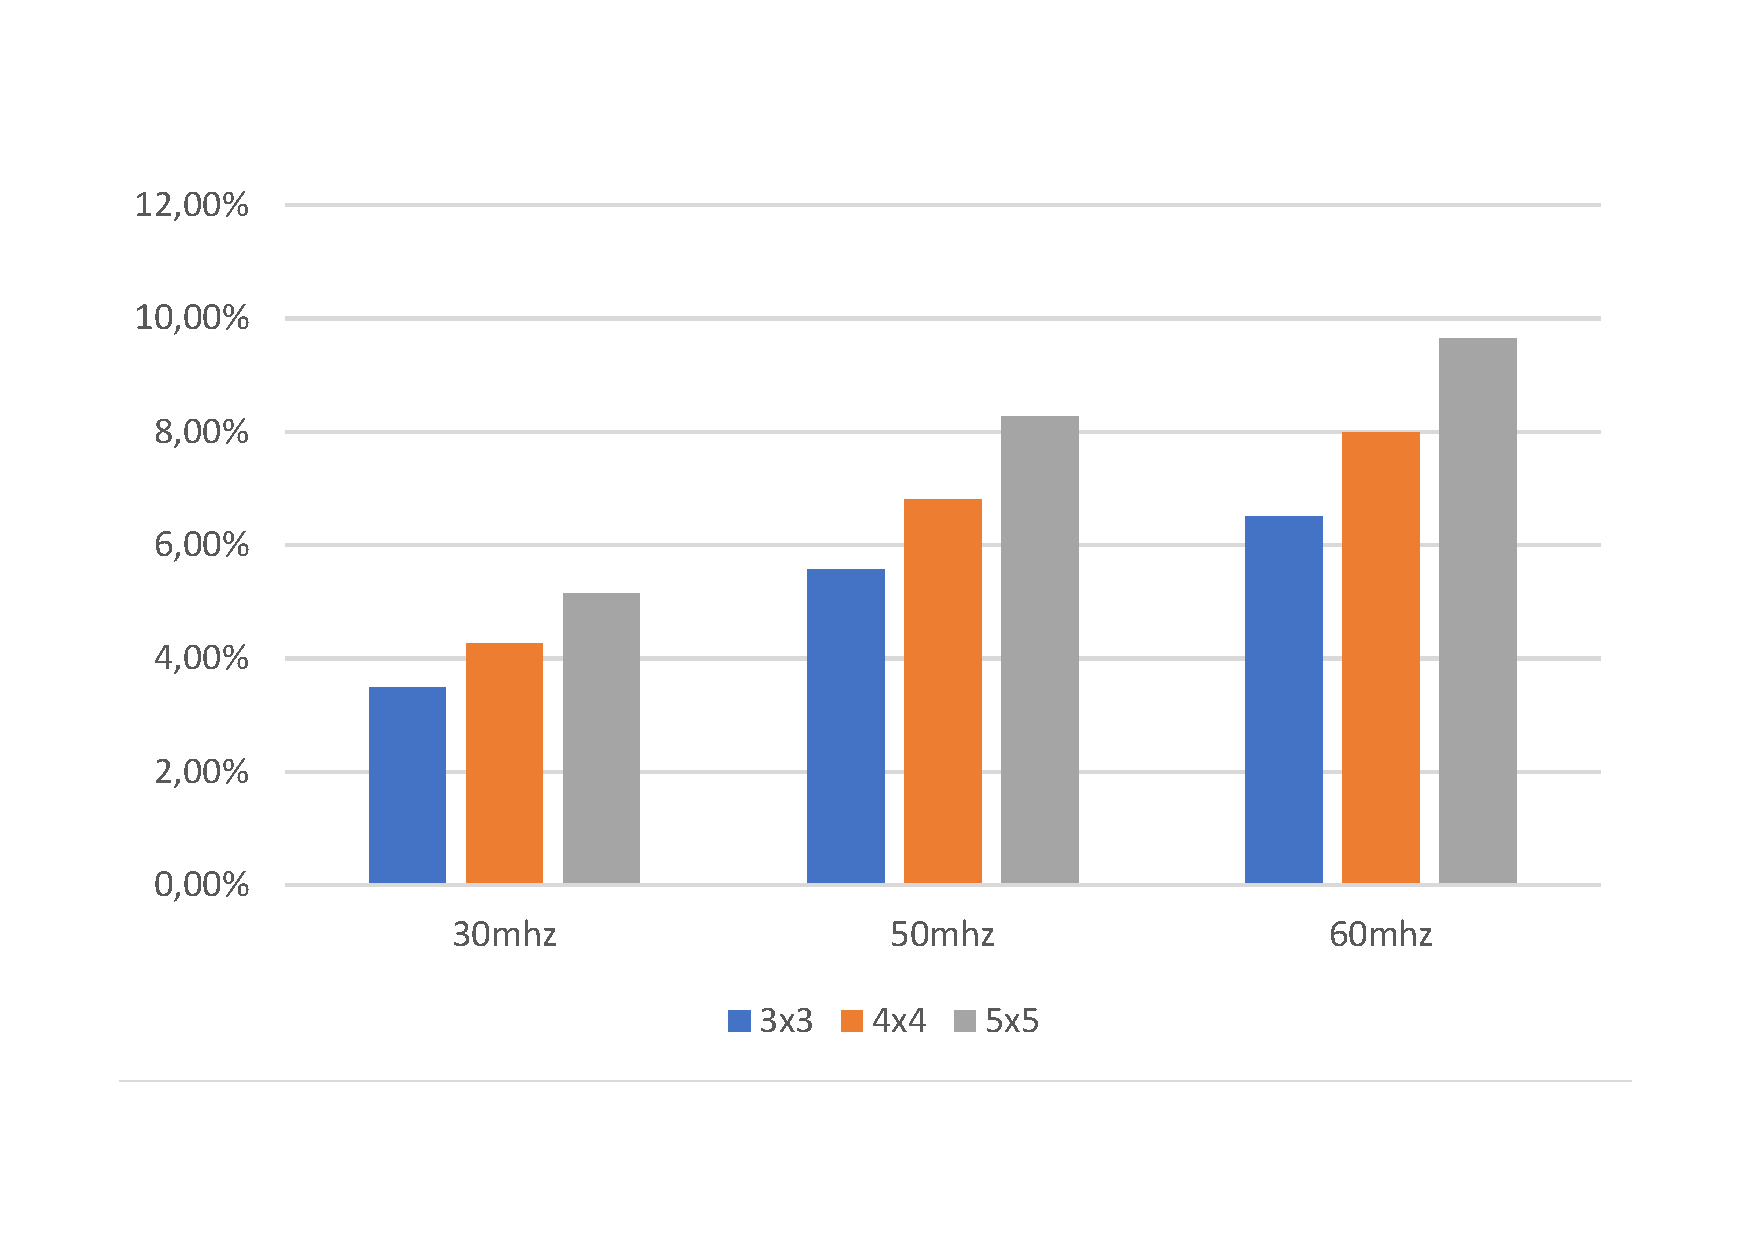
\includegraphics[scale=0.5,angle=0]{./figure/graphs/power_pldyn_int64_freq.pdf}
\caption{Post Implementation Dynamic Power Consumption per Programmable logic with integer 64 PEs}
\label{fig:dynpowint64}
\end{figure}
\begin{figure}[!htbp]
\centering
\captionsetup{justification=centering}
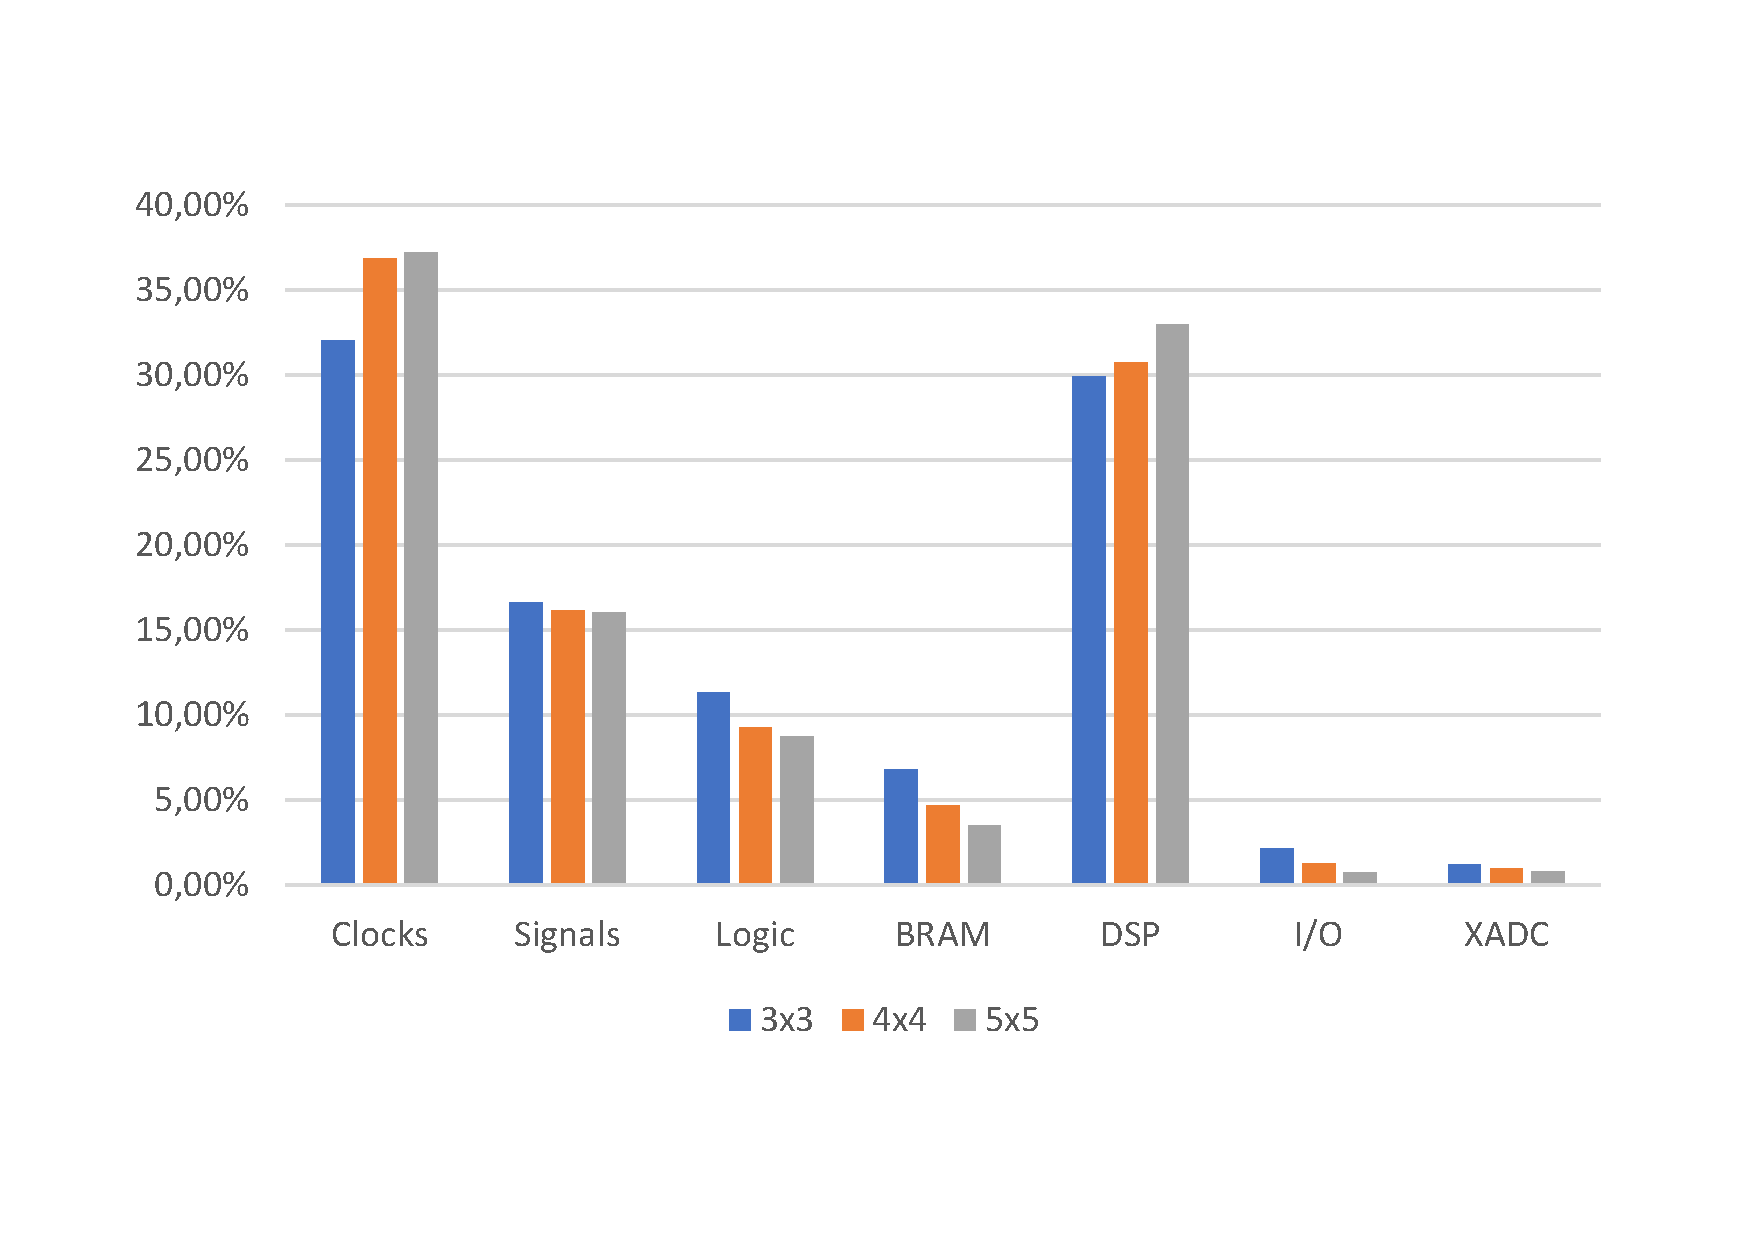
\includegraphics[scale=0.6,angle=0]{./figure/graphs/power_pldyn_div_int64_freq_30mhz.pdf}
\caption{Post Implementation Dynamic Power Consumption per entities in Programmable Logic with a clock frequency of 30 MHz and integer 64 PEs}
\label{fig:dynpowint64ent30}
\end{figure}
\begin{figure}[!htbp]
\centering
\captionsetup{justification=centering}
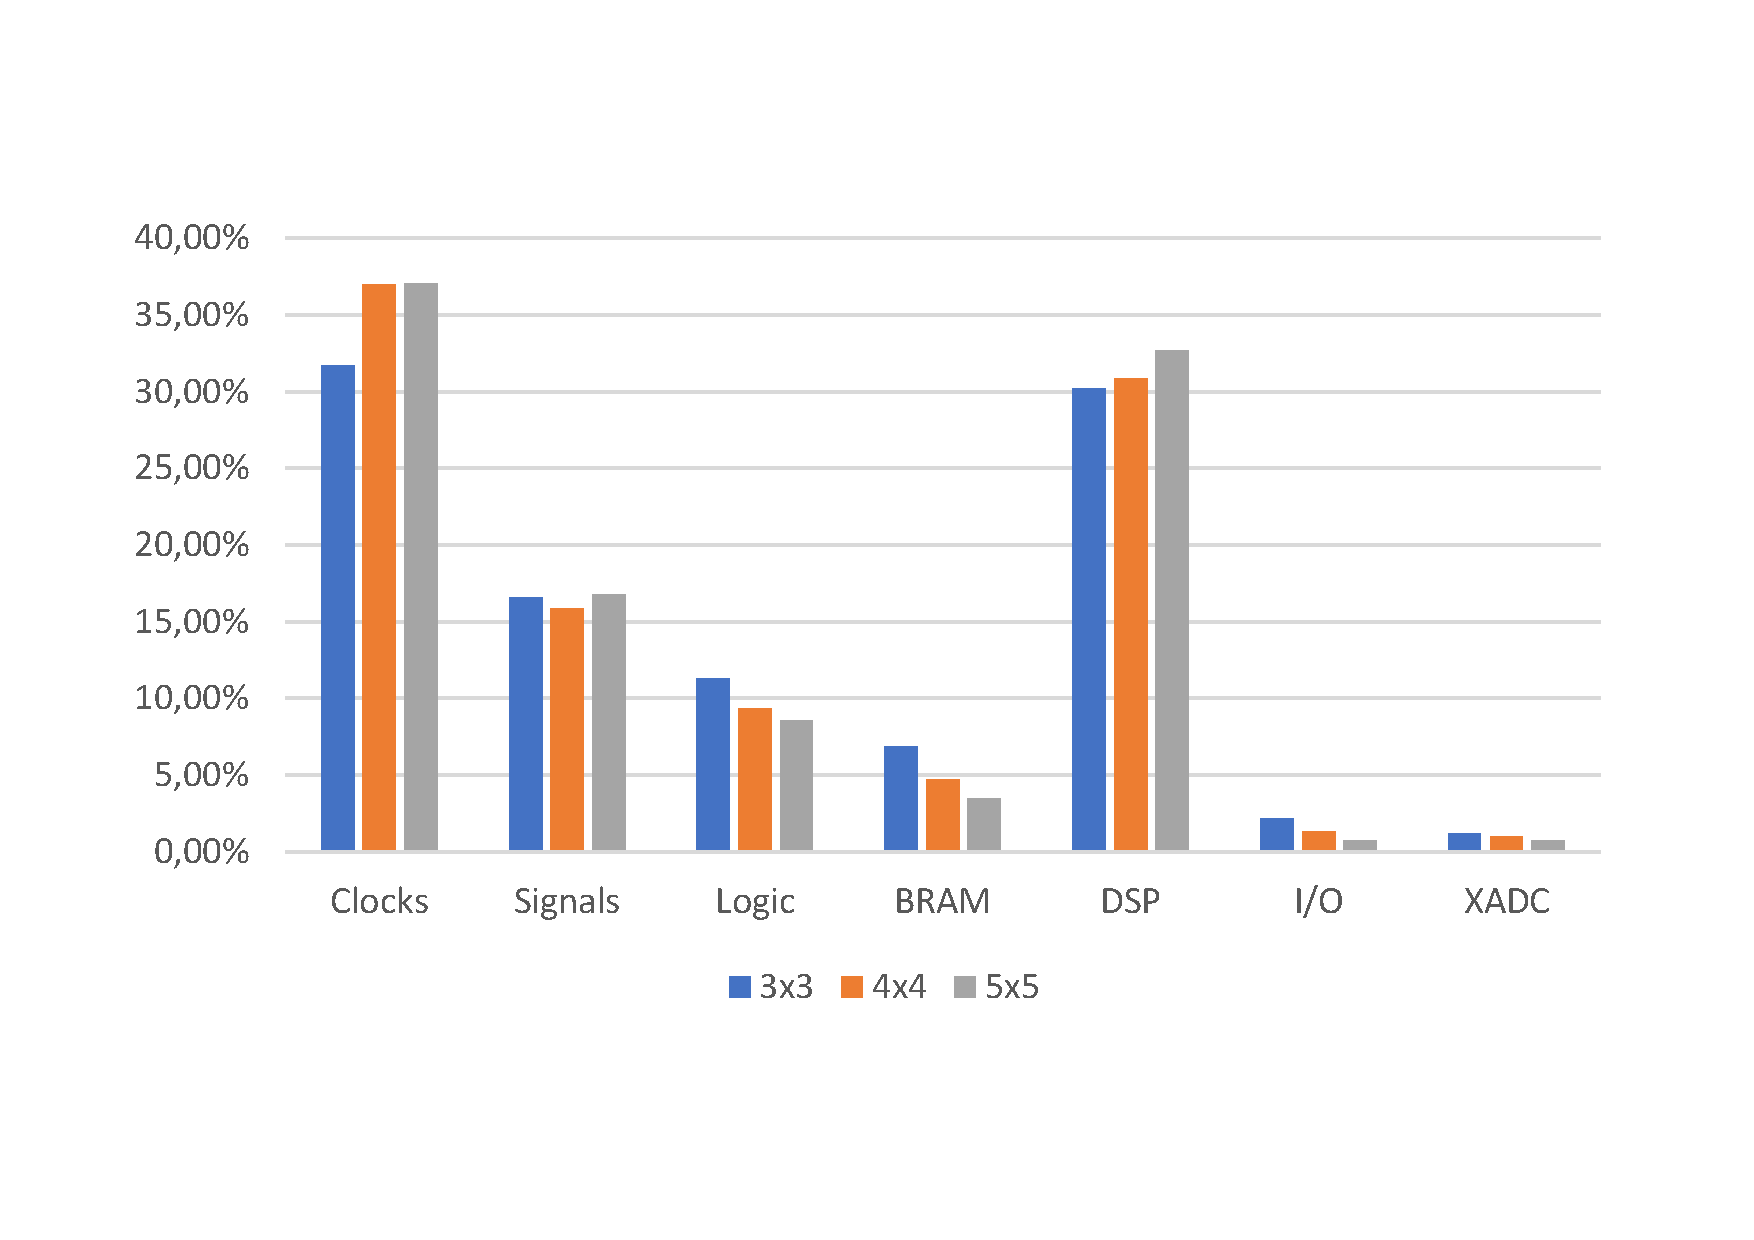
\includegraphics[scale=0.6,angle=0]{./figure/graphs/power_pldyn_div_int64_freq_50mhz.pdf}
\caption{Post Implementation Dynamic Power Consumption per entities in Programmable Logic with a clock frequency of 50 MHz and integer 64 PEs}
\label{fig:dynpowint64ent50}
\end{figure}
\begin{figure}[!htbp]
\centering
\captionsetup{justification=centering}
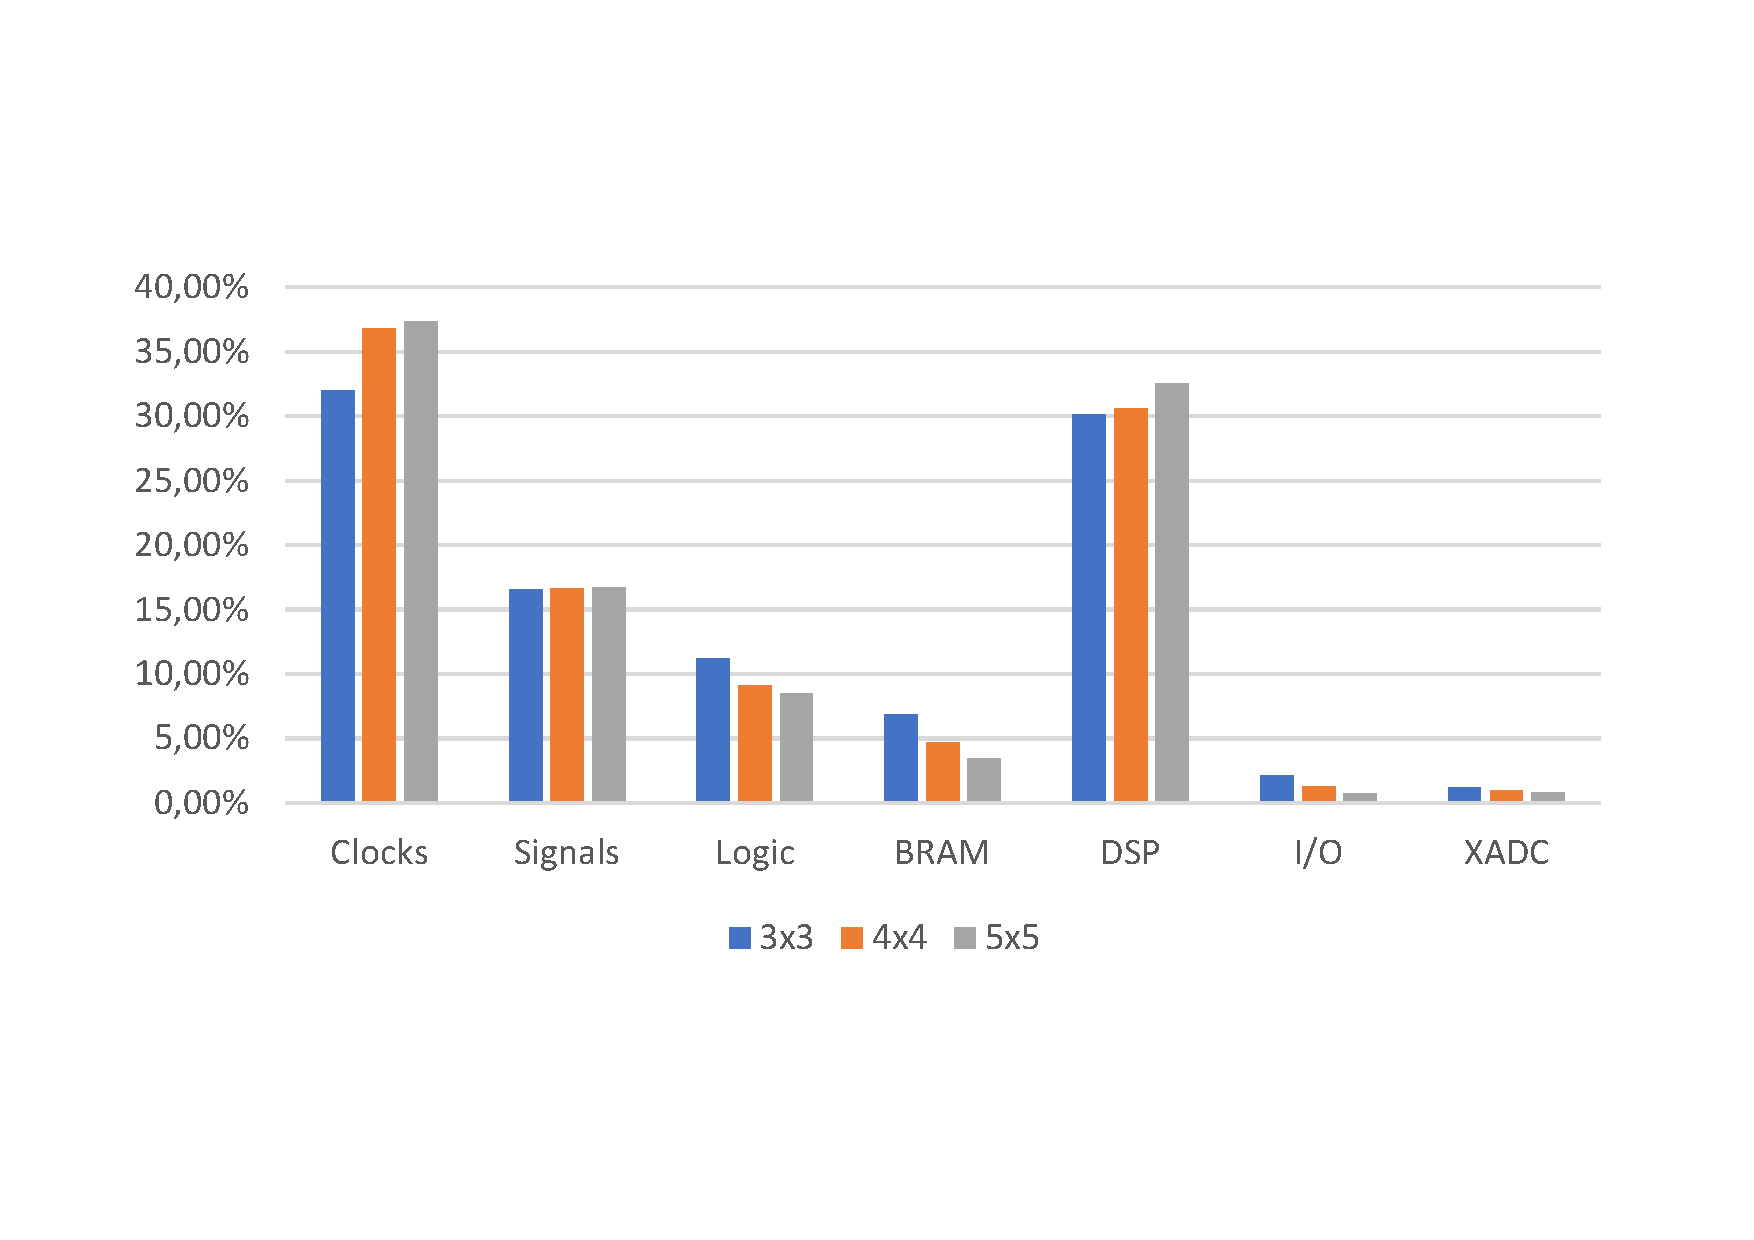
\includegraphics[scale=0.6,angle=0]{./figure/graphs/power_pldyn_div_int64_freq_60mhz.pdf}
\caption{Post Implementation Dynamic Power Consumption per entities in Programmable Logic with a clock frequency of 60 MHz and integer 64 PEs}
\label{fig:dynpowint64ent60}
\end{figure}

As mentioned in the Utilization chapter, the PEs on 64 bit integer are using 14 DSP entities (for having the possibility to compute vectorized operations on data). Therefore, this heavy utilization per PEs is impacting also the power consumed by the DSPs but as it can be seen in Figures fromi \ref{fig:dynpowint64ent30} to \ref{fig:dynpowint64ent60}.
\newpage
\item Brain floating point 16:
\begin{figure}[!htbp]
\centering
\captionsetup{justification=centering}
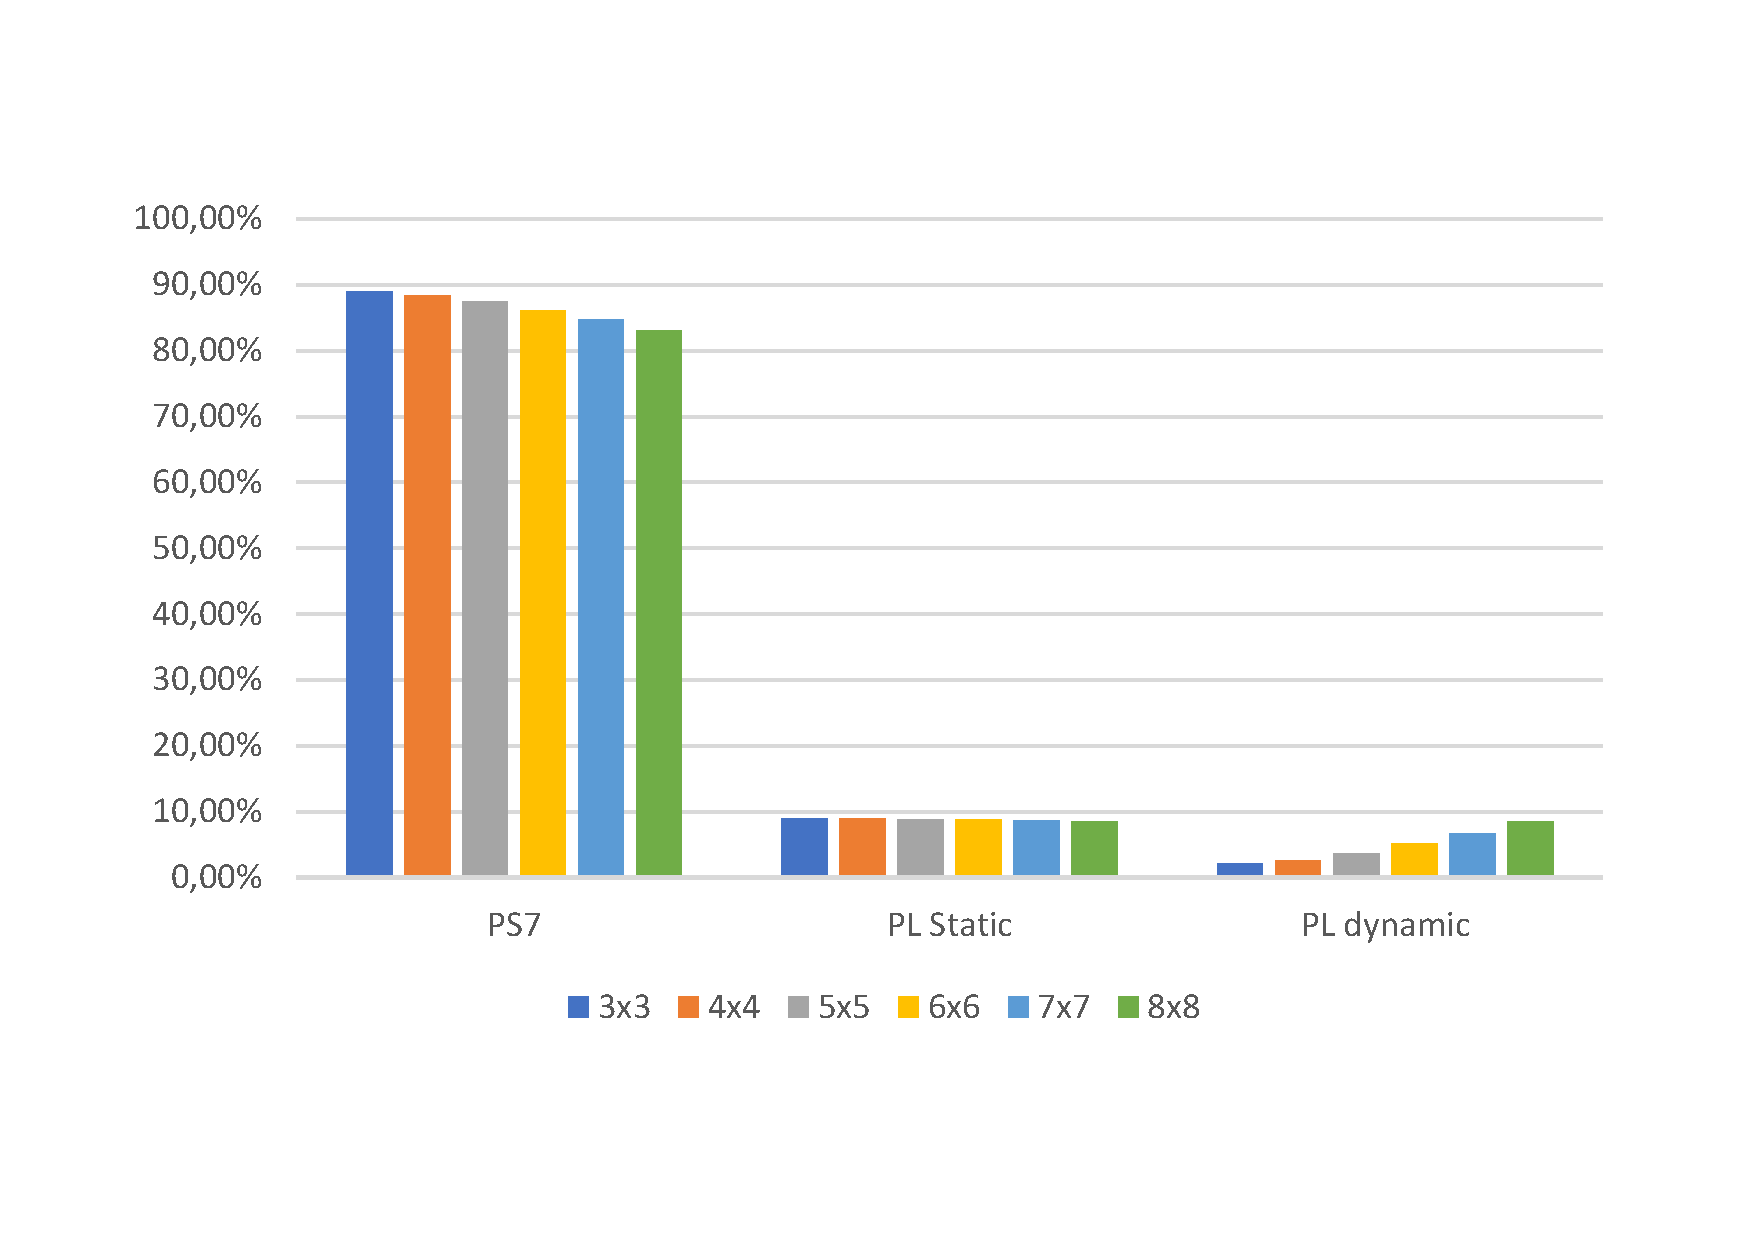
\includegraphics[scale=0.5,angle=0]{./figure/graphs/power_bfp16_freq.pdf}
\caption{Post Implementation Power Consumption for bfp16 PEs}
\label{fig:powbfp16}
\end{figure}
\begin{figure}[!htbp]
\centering
\captionsetup{justification=centering}
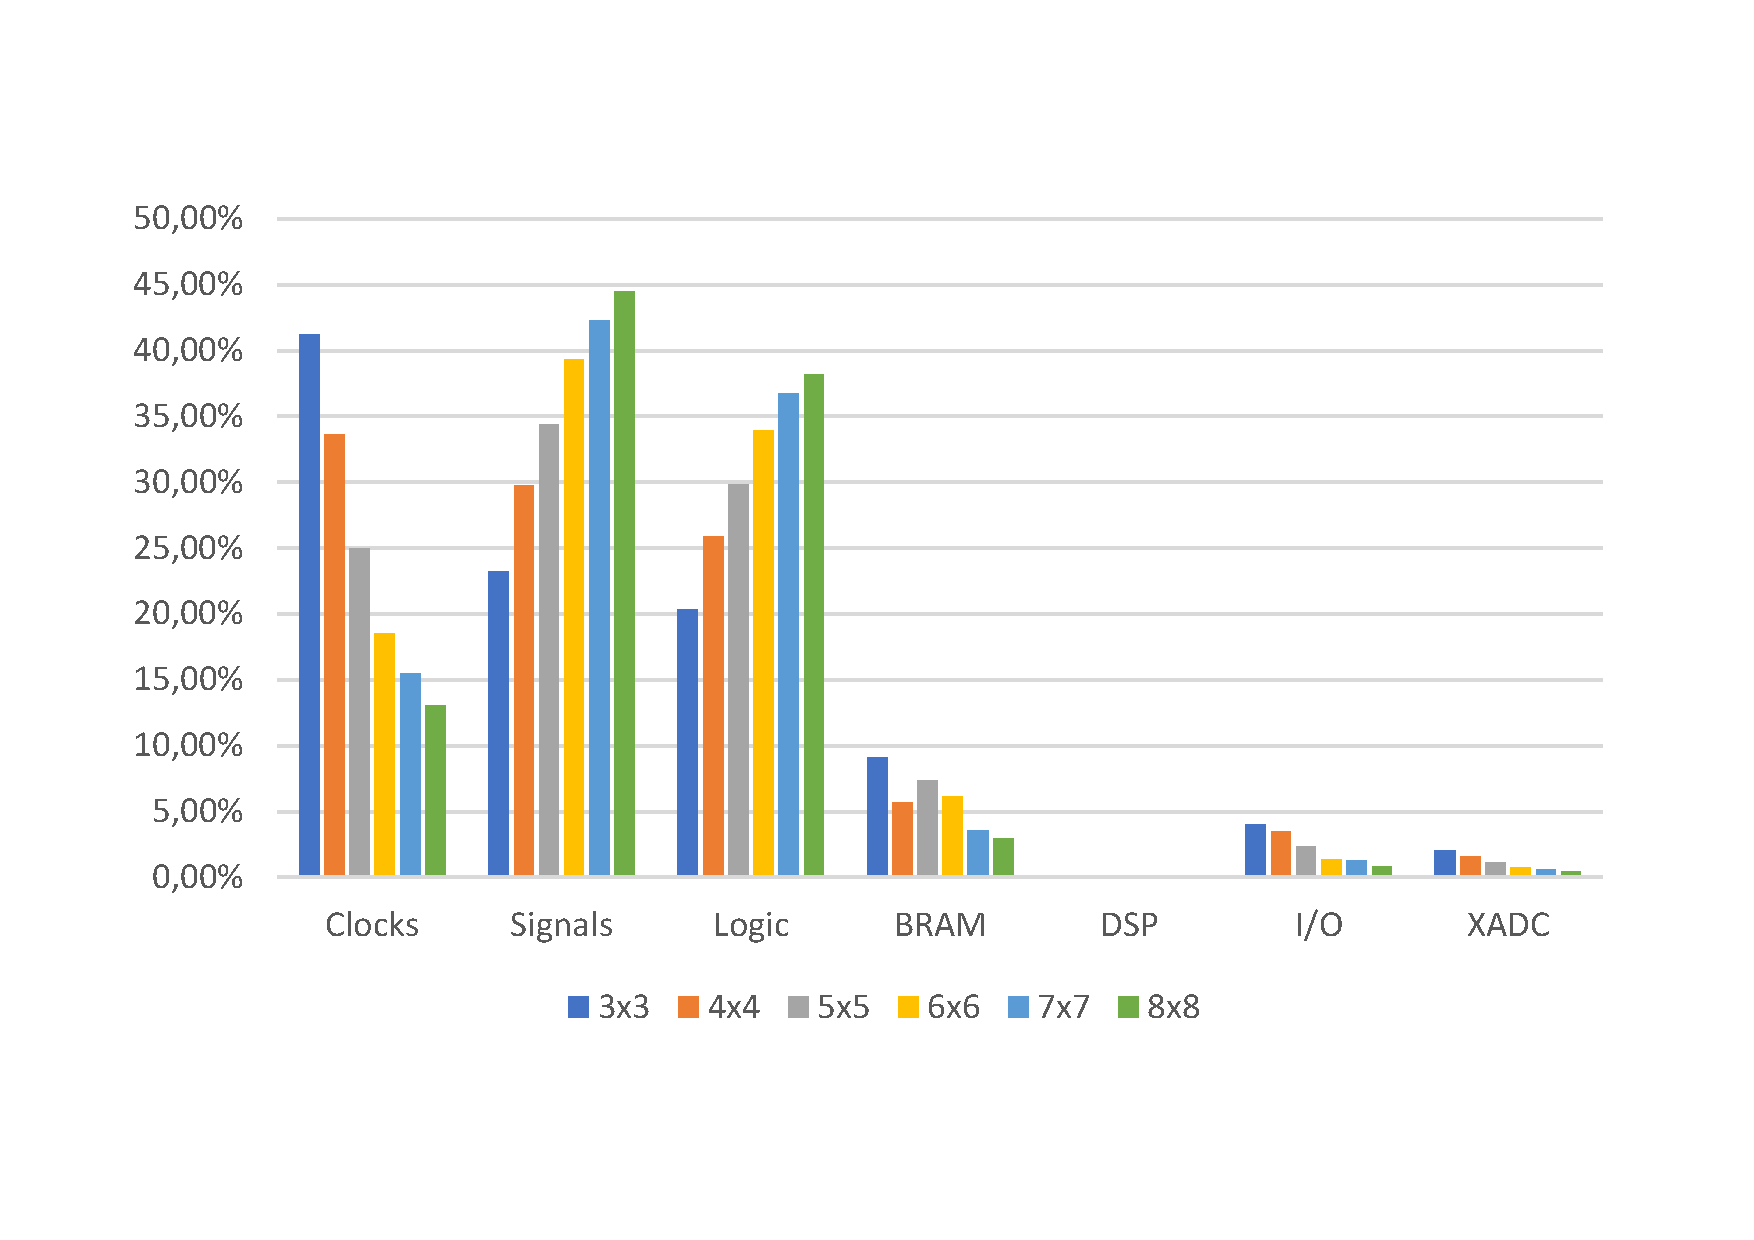
\includegraphics[scale=0.5,angle=0]{./figure/graphs/power_pldyn_div_bfp16_freq_30mhz.pdf}
\caption{Post Implementation Dynamic Power Consumption per entities in Programmable Logic with a clock frequency of 30 MHz and bfp16 PEs}
\label{fig:dynpowintbfp16ent30}
\end{figure}
\newpage
\item Floating point 32: 
\begin{figure}[!htbp]
\centering
\captionsetup{justification=centering}
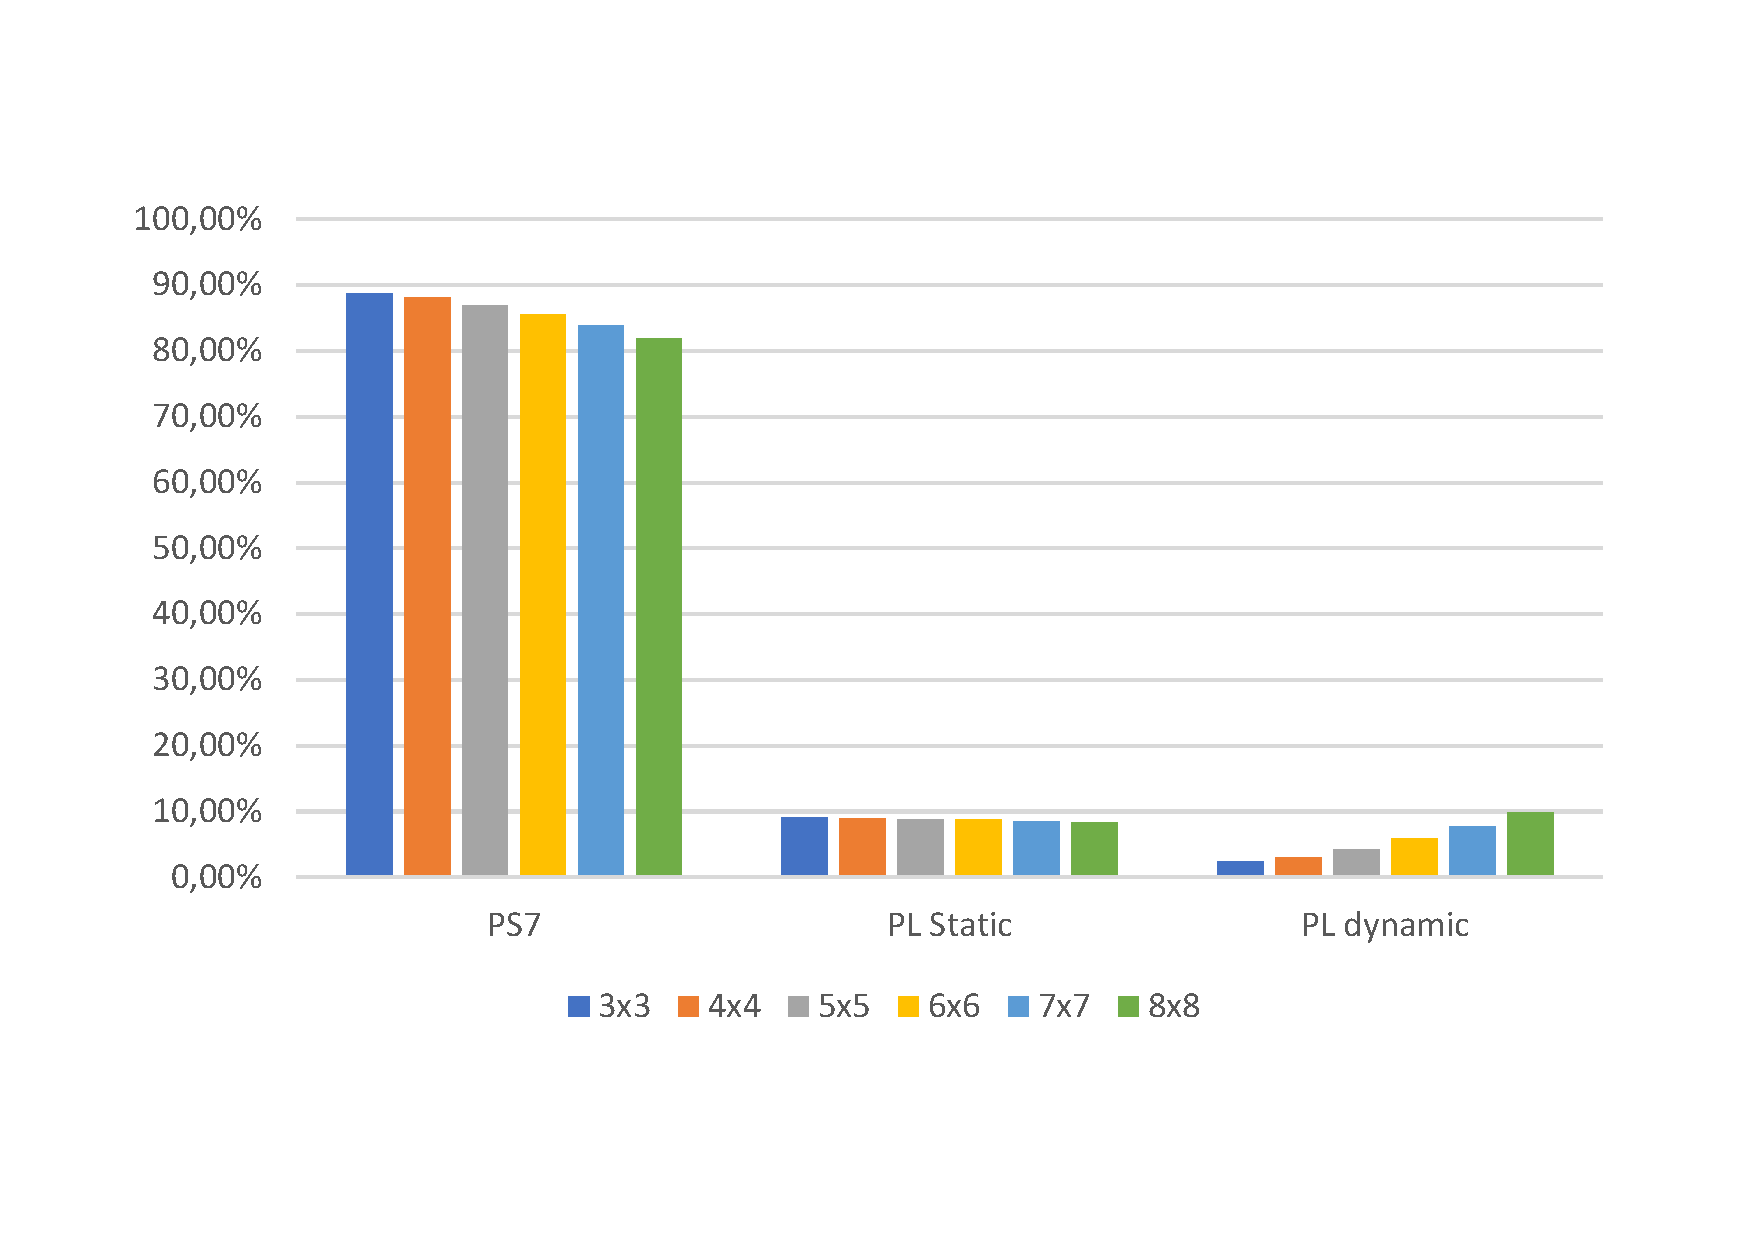
\includegraphics[scale=0.47,angle=0]{./figure/graphs/power_fp32_freq.pdf}
\caption{Post Implementation Power Consumption for fp32 PEs}
\label{fig:powfp32}
\end{figure}
\begin{figure}[!htbp]
\centering
\captionsetup{justification=centering}
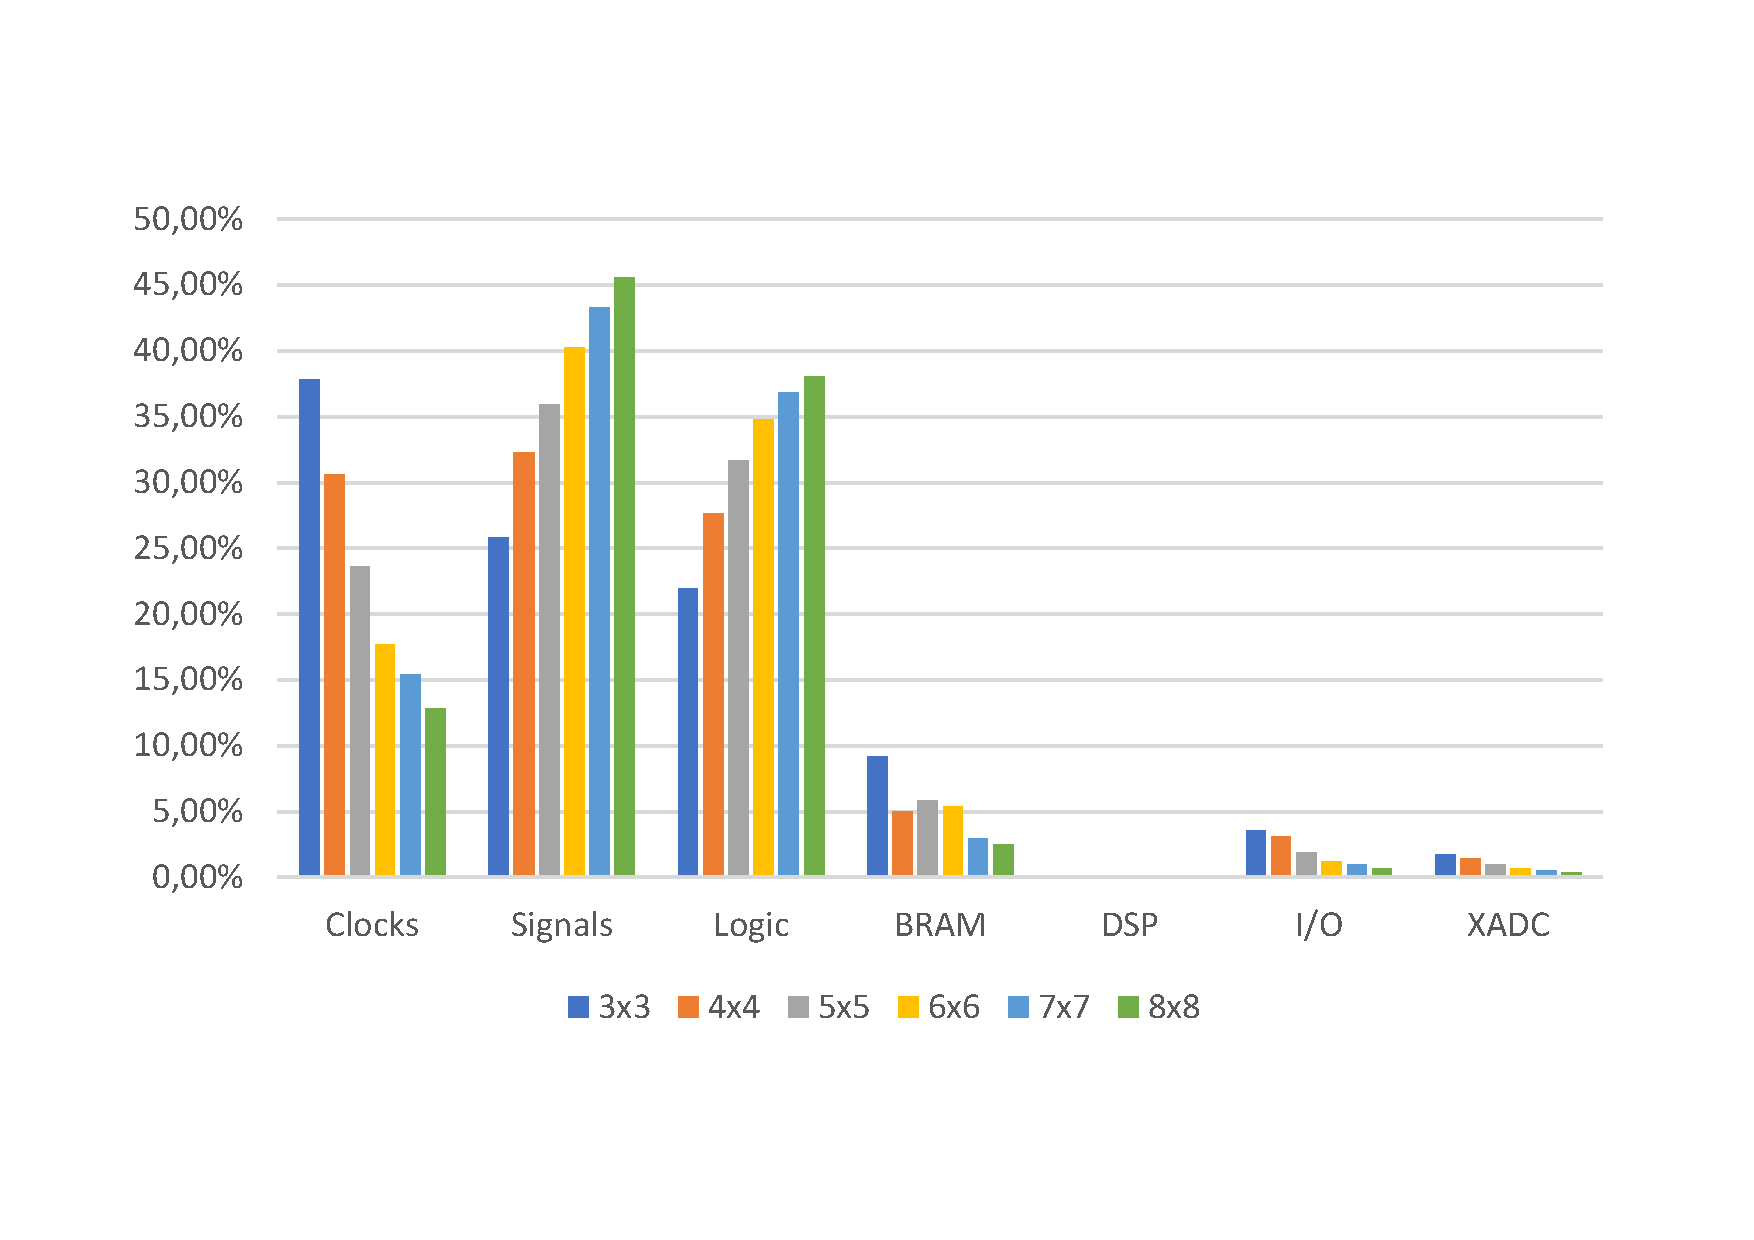
\includegraphics[scale=0.47,angle=0]{./figure/graphs/power_pldyn_div_fp32_freq_30mhz.pdf}
\caption{Post Implementation Dynamic Power Consumption per entities in Programmable Logic with a clock frequency of 30 MHz and fp32 PEs}
\label{fig:dynpowintfp32ent30}
\end{figure}\\
For the bfp16 and fp32 it can be seen that the majority of the power is consumed by the interconnections and the logic. Mainly, because the PEs are implemented in logic.
\end{itemize}
\newpage
Until now, the focus has been on how much the single entities and the different type of power were impacting the total power consumption. It is also worth to compare the absolute values for different data precision, as in the Figure \ref{fig:dynpowcomparisonent3033}.\\
\begin{figure}[!htbp]
\centering
\captionsetup{justification=centering}
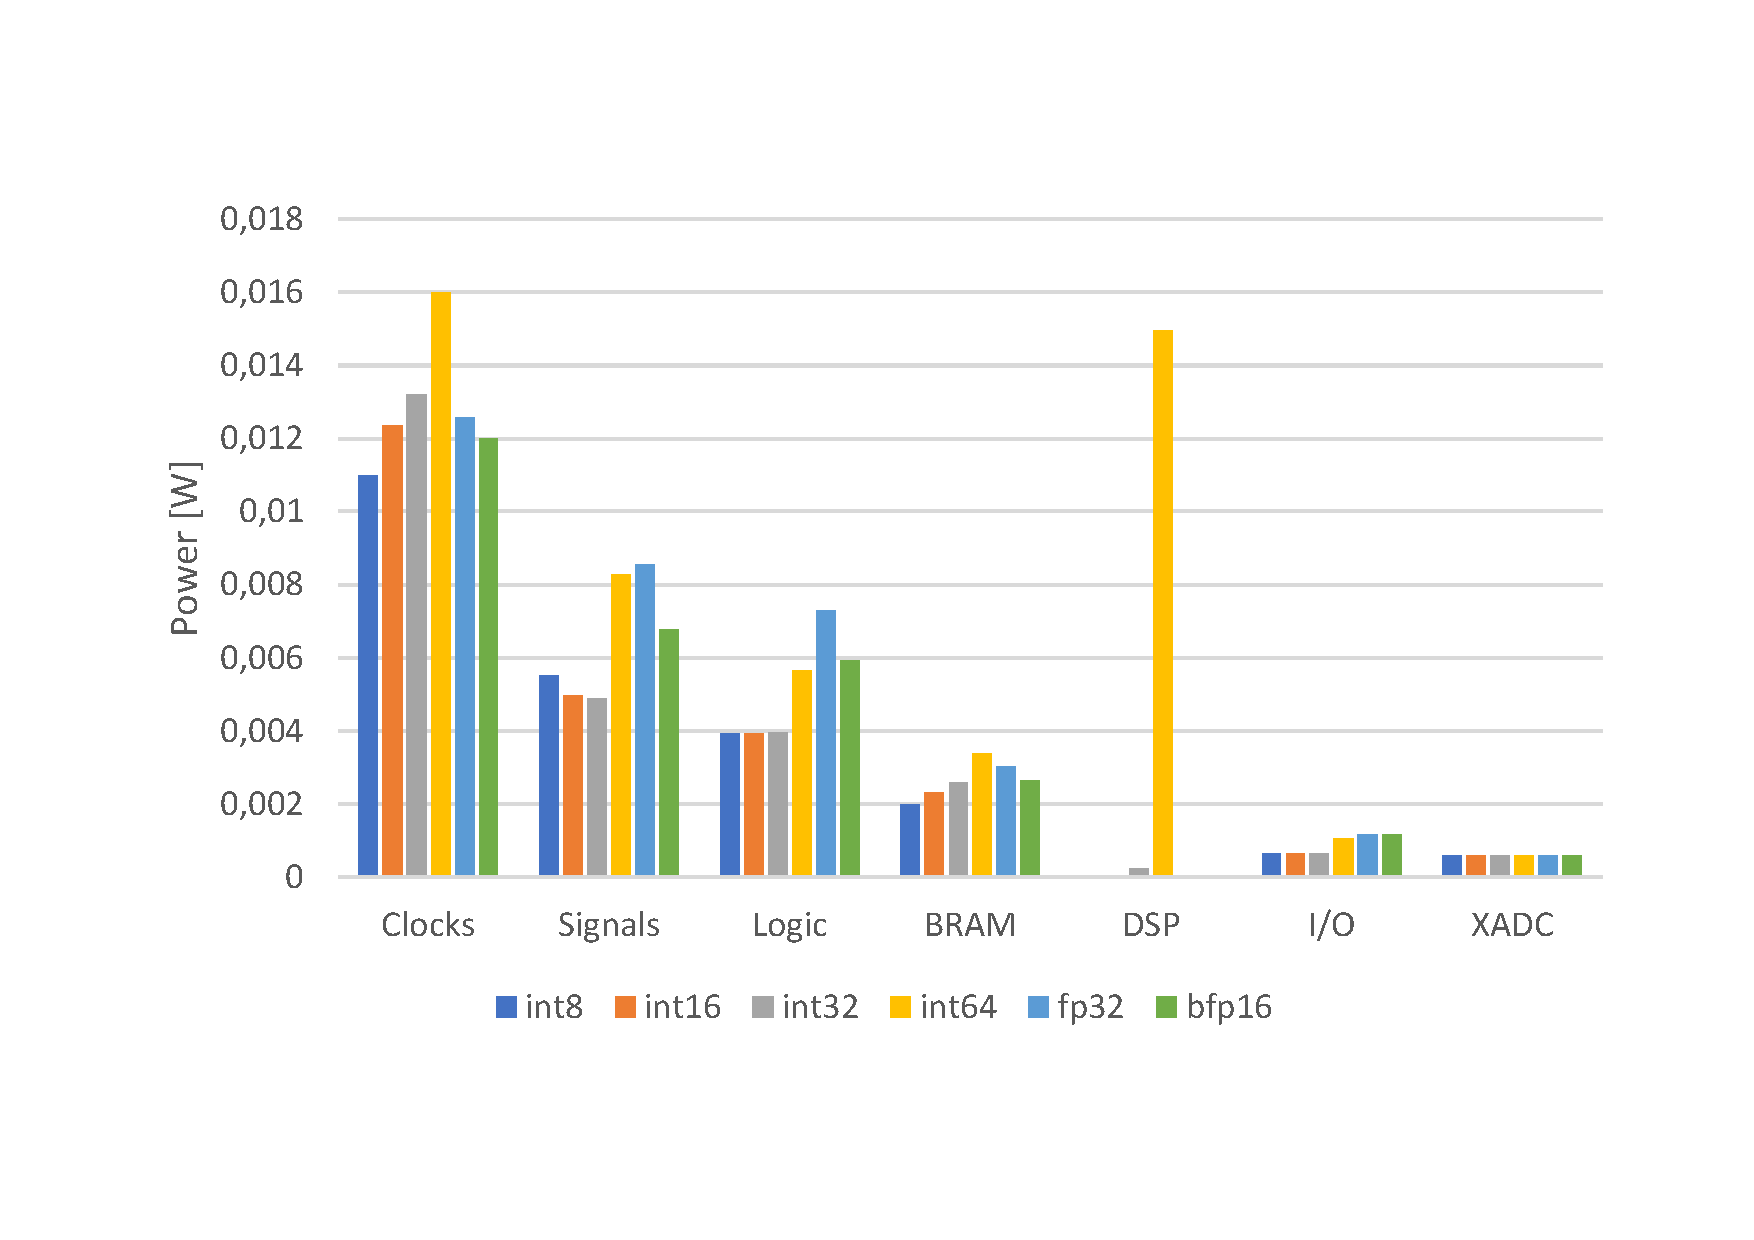
\includegraphics[scale=0.5,angle=0]{./figure/graphs/power_dyn_comparison_pes_30mhz_3x3.pdf}
\caption{Comparison of Post Implementation Dynamic Power Consumption per entities in Programmable Logic with a clock frequency of 30 MHz and a MXU 3x3}
\label{fig:dynpowcomparisonent3033}
\end{figure}\\
As it is very well known from literature and it has also been evident from the other figures and observations, the power consumption per entities grows with the increase of the bitwidth (in the case of integer) and complexity (in the case of floating point).\\
The power consumed by the DSPs (entities in which the integer PEs are implemented in) is negligible for the integer 8 and 16 while it starts to grow slowly using the integer 32 but it explodes with the 64 bit PEs. The high utilization of those PEs leads also to a huge impact in their power consumption.

\todo{should we add the runtime measurement?}

\newpage

\section{Throughput}
According to the definition, the Throughput is the amount of units of information a system can process in a given time. As said that, for the designed accelerator, it results to be equal to the number of rows into the Matrix Multiplication Unit. Normalizing this value with the clock frequency, it results to be constant for all the data type and frequencies.
\begin{figure}[!htbp]
\centering
\captionsetup{justification=centering}
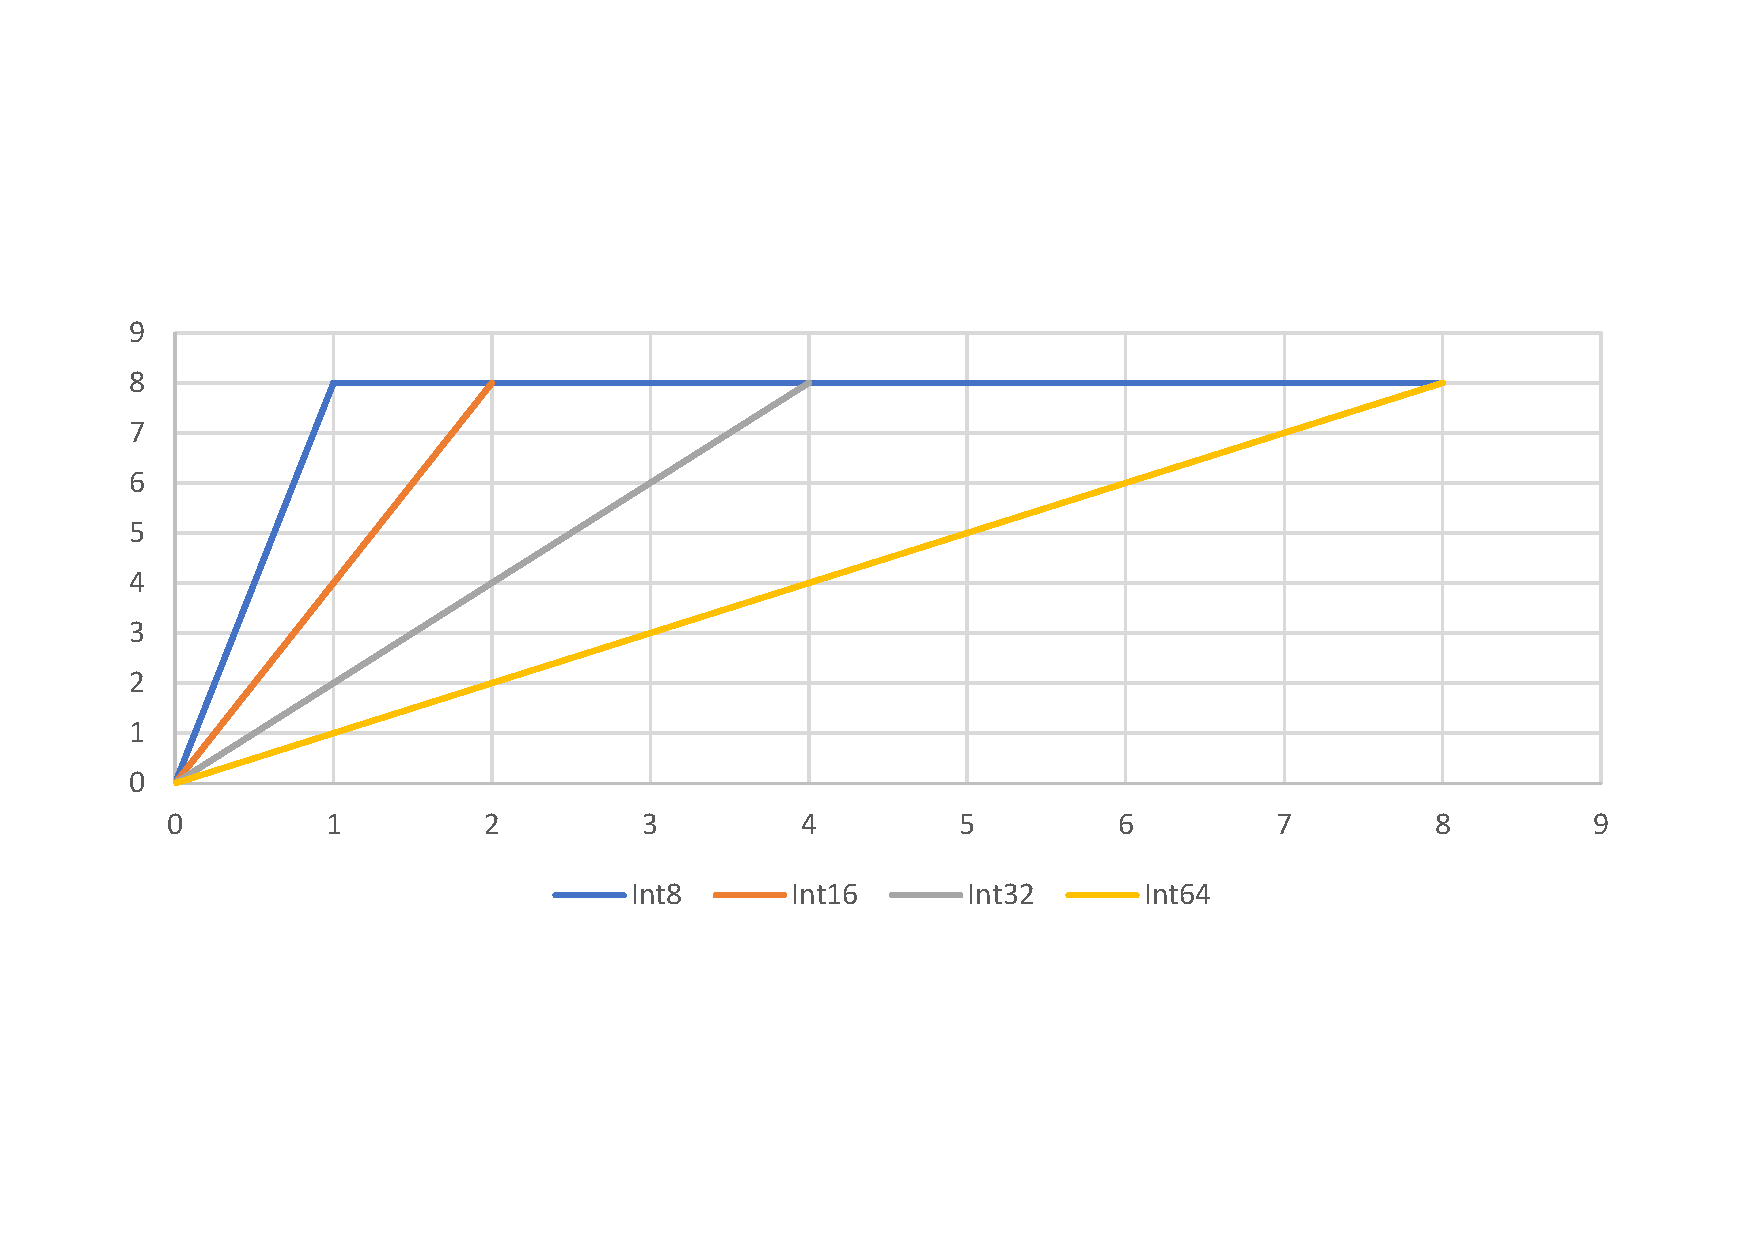
\includegraphics[scale=0.45,angle=0]{./figure/graphs/roofline.pdf}
\caption{Roofline model of the accelerator with a MXU size of 8x8}
\label{fig:roofline}
\end{figure}

The theoretical throughput given by the roofline model (Figure \label{fig:roofline}) and it is equal to the number of rows in the matrix multiplication unit. The assumption is that enough data are provided to the accelerator in order to have all the Processing Elements working with useful data, if the latter is not meet the throughput goes down.
In Figure \label{fig:roofline} the different slopes for different data width are representing the different number of internal memory accessess in order to retrieve data for all the Processing Elements.\\

The throughput can be further increased in the 64-bitwidth configuration of the Processing Elements. As already mentioned, those 64-bit units are able to compute vectorized instructions and therefore increase the number of computation per cycle. However, this comes with the overhead of more memory accesses as it can be apprecieted in the \label{fig:rooflinevect}.

\begin{figure}[!htbp]
\centering
\captionsetup{justification=centering}
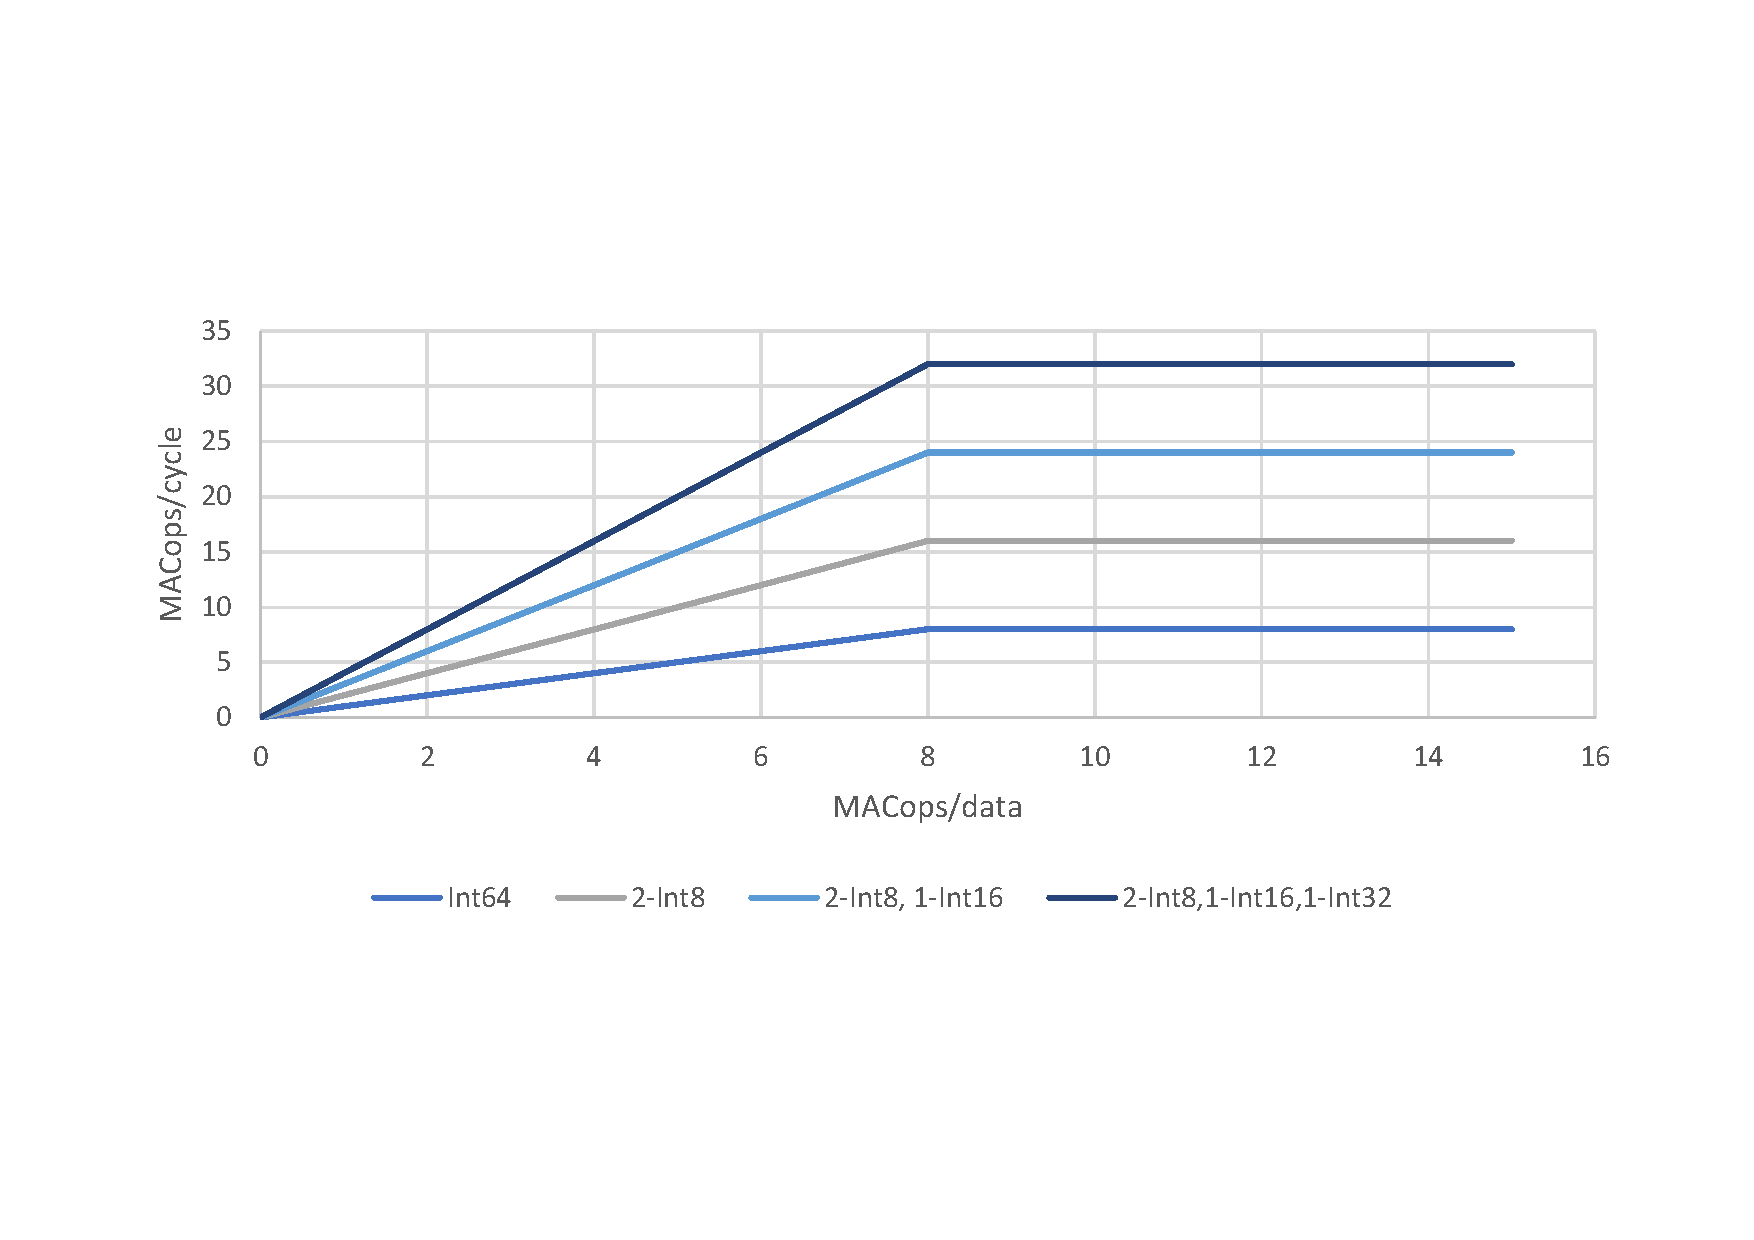
\includegraphics[scale=0.45,angle=0]{./figure/graphs/roofline_vectorized.pdf}
\caption{Roofline model of the accelerator with a MXU size of 8x8 and vectorized PEs}
\label{fig:rooflinevect}
\end{figure}
 \newpage
 
\section{Latency}
In a real time application, the most important factor is the latency, the execution time of a task.
In this case the latency is measured as average of the execution time of a Neural Network model for different platforms. In addition, the execution of the models, on the target, in the configuration \textit{CPU+accelerator} is done with different clock frequencies and data type in the Programmable Logic, and as consequence a different overall latency (and power consumption).\\
In the following tables, the execution type for different data type and model is presented (with a fixed clock frequency of the accelerator at 80 MHz).
\begin{center}
\begin{table}[!htbp]
\centering
\captionsetup{justification=centering}
\begin{tabular}{ |p{2.5cm}||p{2.5cm}|p{2.5cm}|p{2.5cm}|p{2.5cm}| }
\hline
Model & CPU (host)\protect\footnotemark[1] & GPU(host)\protect\footnotemark[2] & CPU(Pynq Z2 board)\protect\footnotemark[3] & CPU(Pynq Z2 board) + accelerator \\
\hline
MNIST & 0.3 ms & 5.7 ms & 2.9 ms  & \\
\hline
Cifar 10& 20 ms & 22 ms& 160 ms &\\
\hline
\end{tabular}
\caption{Execution Time for different platform and model, integer 8}
\label{table:moplatint8}
\end{table}
\end{center}

\begin{center}
\begin{table}[!htbp]
\centering
\captionsetup{justification=centering}
\begin{tabular}{ |p{2.5cm}||p{2.5cm}|p{2.5cm}|p{2.5cm}|p{2.5cm}| }
\hline
Model & CPU (host)\protect\footnotemark[1] & GPU(host)\protect\footnotemark[2] & CPU(Pynq Z2 board)\protect\footnotemark[3] & CPU(Pynq Z2 board) + accelerator \\
\hline
MNIST & 0.3 ms & 5.7 ms & 2.9 ms  & \\
\hline
Cifar 10& 20 ms & 22 ms& 160 ms &\\
\hline
\end{tabular}
\caption{Execution Time for different platform and model, integer 16}
\label{table:moplatint16}
\end{table}
\end{center}
\begin{center}
\begin{table}[!htbp]
\centering
\captionsetup{justification=centering}
\begin{tabular}{ |p{2.5cm}||p{2.5cm}|p{2.5cm}|p{2.5cm}|p{2.5cm}| }
\hline
Model & CPU (host)\protect\footnotemark[1] & GPU(host)\protect\footnotemark[2] & CPU(Pynq Z2 board)\protect\footnotemark[3] & CPU(Pynq Z2 board) + accelerator \\
\hline
MNIST & 0.3 ms & 5.7 ms & 2.9 ms  & \\
\hline
Cifar 10& 20 ms & 22 ms& 160 ms &\\
\hline
\end{tabular}
\caption{Execution Time for different platform and model, integer 32}
\label{table:moplatint32}
\end{table}
\end{center}
\todo{divide the execution time in percentage and check how the time is divided} 


\todo{graph of how the execution time on the target changes with the frequency for every model}
\footnotetext[1]{Intel i7-6700HQ, 2.60 Ghz}
\footnotetext[2]{NVIDIA, GeForce GTX960M, 1.176 Ghz }
\footnotetext[3]{Arm dual-core Cortex-A9, 650 MHz }

On the other hand, the clock frequency of the accelerator can be tuned. Therefore, in the following, the behavior of the latency for every model with changing in the clock frequency is presented.
\todo{a possible estimation of the speedup}

\newpage

\section{Accuracy}
The accuracy of inference process in Machine Learning model is how much the prediction is close to the actual value. For example, using the MNIST model, how much is accurate the predicion of a number giving the number as input to the Neural Network. \\ 
In the following case, the accuracy for different data width and model will be presented with reference to the actual value, in this case the inference without the hardware accelerator. Moreover, the data provided to the accelerator are bounded by the filter size of the weight, which is always fixed to 3x3 for the used models. Therefore, the MXU for the following comparison has been the standard one, the 8x8.
\begin{center}
\begin{table}[!htbp]
\centering
\captionsetup{justification=centering}
\begin{tabular}{ |P{2cm}||P{1.8cm}|P{2.2cm}|P{2.2cm}|P{2.2cm}|P{1.8cm}| }
\hline
Model &  $\leq\pm5\%$ &  $\pm5\%\div25\%$ & $\pm25\%\div50\%$ & $\pm50\%\div75\%$ &  $\geq\pm75\%$ \\ 
\hline
MNIST &   & & x & &\\ 
\hline
Cifar 10& & & & &x \\
\hline
\end{tabular}
\caption{Accuracy Output\protect\footnotemark[1]  with Convolution on integer 8 }
\label{table:accuracyint8}
\end{table}
\end{center}
\begin{center}
\begin{table}[!htbp]
\centering
\captionsetup{justification=centering}
\begin{tabular}{ |P{2cm}||P{1.8cm}|P{2.2cm}|P{2.2cm}|P{2.2cm}|P{1.8cm}| }
\hline
Model &  $\leq\pm5\%$ &  $\pm5\%\div25\%$ & $\pm25\%\div50\%$ & $\pm50\%\div75\%$ &  $\geq\pm75\%$ \\ 
\hline
MNIST &   & & & x &\\ 
\hline
Cifar 10& & & &x &   \\
\hline
\end{tabular}
\caption{Accuracy Output\protect\footnotemark[1]  with Convolution on integer 16 }
\label{table:accuracyint16}
\end{table}
\end{center}

\begin{center}
\begin{table}[!htbp]
\centering
\captionsetup{justification=centering}
\begin{tabular}{ |P{2cm}||P{1.8cm}|P{2.2cm}|P{2.2cm}|P{2.2cm}|P{1.8cm}| }
\hline
Model &  $\leq\pm5\%$ &  $\pm5\%\div25\%$ & $\pm25\%\div50\%$ & $\pm50\%\div75\%$ &  $\geq\pm75\%$ \\ 
\hline
MNIST &   & & &x & \\ 
\hline
Cifar 10& & & &&x \\
\hline
\end{tabular}
\caption{Accuracy Output\protect\footnotemark[1]  with Convolution on integer 32 }
\label{table:accuracyint32}
\end{table}
\end{center}

It comes suddenly evident that the output prediction with the accelerator integrated varies of a huge amount from the expected one. \\
One of the reason of the wrong prediction may reside in the input data feed to the model, they are totally random. Being feed with random, and probably unreasonable, data the prediction accuracy has been degradeted.
Another improvement from the hardware point of view, which could improve the output accuracy, should be to accumulate on the different bitwidth precision, for example compute multiplication on 8 bits integer and accumulate values on 16 bit integer. Moreover, as in every software product, bugs have not been detected but this does not means that the written software is bug-free.

\footnotetext[1]{The accuracy is measured percentage(wrt the reference accuracy) of the difference between the reference accuracy (the model's output on the CPU only execution) and the output accuracy of the CPU+ hardware accelerator of the main predicion, the higher one. }
